\documentclass[compress,aspectratio=1610]{beamer}

%\usepackage[utf8]{inputenc}
%\usepackage[T1]{fontenc}
%\usepackage[ngerman]{babel}
%\usepackage{hyphenat}
%\inputencoding{utf8}
%\makeatother

\usepackage[english]{babel}
\usepackage[english]{isodate}
\isodate
\usepackage{multicol}

\usepackage{csquotes}

\usepackage{amsmath}
\usepackage{amssymb}
\usepackage{slashed}
\usepackage{mathtools}

\usepackage{xfrac}

\usepackage[export]{adjustbox}
\usepackage{graphicx}
\usepackage{overpic}
\DeclareGraphicsExtensions{.png}
\graphicspath{{../img/}{../img/defence/}}

\usepackage{tikz}
\usetikzlibrary{calc,shapes,arrows,positioning}

\usetheme{vertex}

\usepackage{booktabs}

\usepackage{ifthen}
\newboolean{uprightparticles}
\setboolean{uprightparticles}{false}
%%% $Id: lhcb-symbols-def.tex 115102 2017-11-22 09:15:01Z fwilson $
%%% ======================================================================
%%% Purpose: Standard LHCb aliases
%%% Author: Originally Ulrik Egede, adapted by Tomasz Skwarnicki for templates,
%%% rewritten by Chris Parkes
%%% Maintainer : Ulrik Egede (2010 - 2012)
%%% Maintainer : Rolf Oldeman (2012 - 2014)
%%% =======================================================================

%%% To use this file outside the normal LHCb document environment, the
%%% following should be added in a preamble (before \begin{document}
%%%
%%%\usepackage{ifthen} 
%%%\newboolean{uprightparticles}
%%%\setboolean{uprightparticles}{false} %Set true for upright particle symbols
\usepackage{xspace} 
\usepackage{upgreek}

%%%%%%%%%%%%%%%%%%%%%%%%%%%%%%%%%%%%%%%%%%%%%%%%%%%%%%%%%%%%
%%%
%%% The following is to ensure that the template automatically can process
%%% this file.
%%%
%%% Add comments with at least three %%% preceding.
%%% Add new sections with one % preceding
%%% Add new subsections with two %% preceding
%%%%%%%%%%%%%%%%%%%%%%%%%%%%%%%%%%%%%%%%%%%%%%%%%%%%%%%%%%%%

%%%%%%%%%%%%%
% Experiments
%%%%%%%%%%%%%
\def\lhcb {\mbox{LHCb}\xspace}
\def\atlas  {\mbox{ATLAS}\xspace}
\def\cms    {\mbox{CMS}\xspace}
\def\alice  {\mbox{ALICE}\xspace}
\def\babar  {\mbox{BaBar}\xspace}
\def\belle  {\mbox{Belle}\xspace}
\def\cleo   {\mbox{CLEO}\xspace}
\def\cdf    {\mbox{CDF}\xspace}
\def\dzero  {\mbox{D0}\xspace}
\def\aleph  {\mbox{ALEPH}\xspace}
\def\delphi {\mbox{DELPHI}\xspace}
\def\opal   {\mbox{OPAL}\xspace}
\def\lthree {\mbox{L3}\xspace}
\def\sld    {\mbox{SLD}\xspace}
%%%\def\argus  {\mbox{ARGUS}\xspace}
%%%\def\uaone  {\mbox{UA1}\xspace}
%%%\def\uatwo  {\mbox{UA2}\xspace}
%%%\def\ux85 {\mbox{UX85}\xspace}
\def\cern {\mbox{CERN}\xspace}
\def\lhc    {\mbox{LHC}\xspace}
\def\lep    {\mbox{LEP}\xspace}
\def\tevatron {Tevatron\xspace}

%% LHCb sub-detectors and sub-systems

%%%\def\pu     {PU\xspace}
\def\velo   {VELO\xspace}
\def\rich   {RICH\xspace}
\def\richone {RICH1\xspace}
\def\richtwo {RICH2\xspace}
\def\ttracker {TT\xspace}
\def\intr   {IT\xspace}
\def\st     {ST\xspace}
\def\ot     {OT\xspace}
\def\herschel {\mbox{\textsc{HeRSCheL}}\xspace}
%%%\def\Tone   {T1\xspace}
%%%\def\Ttwo   {T2\xspace}
%%%\def\Tthree {T3\xspace}
%%%\def\Mone   {M1\xspace}
%%%\def\Mtwo   {M2\xspace}
%%%\def\Mthree {M3\xspace}
%%%\def\Mfour  {M4\xspace}
%%%\def\Mfive  {M5\xspace}
\def\spd    {SPD\xspace}
\def\presh  {PS\xspace}
\def\ecal   {ECAL\xspace}
\def\hcal   {HCAL\xspace}
%%%\def\bcm    {BCM\xspace}
\def\MagUp {\mbox{\em Mag\kern -0.05em Up}\xspace}
\def\MagDown {\mbox{\em MagDown}\xspace}

\def\ode    {ODE\xspace}
\def\daq    {DAQ\xspace}
\def\tfc    {TFC\xspace}
\def\ecs    {ECS\xspace}
\def\lone   {L0\xspace}
\def\hlt    {HLT\xspace}
\def\hltone {HLT1\xspace}
\def\hlttwo {HLT2\xspace}

%%% Upright (not slanted) Particles

\ifthenelse{\boolean{uprightparticles}}%
{\def\Palpha      {\ensuremath{\upalpha}\xspace}
 \def\Pbeta       {\ensuremath{\upbeta}\xspace}
 \def\Pgamma      {\ensuremath{\upgamma}\xspace}                 
 \def\Pdelta      {\ensuremath{\updelta}\xspace}                 
 \def\Pepsilon    {\ensuremath{\upepsilon}\xspace}                 
 \def\Pvarepsilon {\ensuremath{\upvarepsilon}\xspace}                 
 \def\Pzeta       {\ensuremath{\upzeta}\xspace}                 
 \def\Peta        {\ensuremath{\upeta}\xspace}                 
 \def\Ptheta      {\ensuremath{\uptheta}\xspace}                 
 \def\Pvartheta   {\ensuremath{\upvartheta}\xspace}                 
 \def\Piota       {\ensuremath{\upiota}\xspace}                 
 \def\Pkappa      {\ensuremath{\upkappa}\xspace}                 
 \def\Plambda     {\ensuremath{\uplambda}\xspace}                 
 \def\Pmu         {\ensuremath{\upmu}\xspace}                 
 \def\Pnu         {\ensuremath{\upnu}\xspace}                 
 \def\Pxi         {\ensuremath{\upxi}\xspace}                 
 \def\Ppi         {\ensuremath{\uppi}\xspace}                 
 \def\Pvarpi      {\ensuremath{\upvarpi}\xspace}                 
 \def\Prho        {\ensuremath{\uprho}\xspace}                 
 \def\Pvarrho     {\ensuremath{\upvarrho}\xspace}                 
 \def\Ptau        {\ensuremath{\uptau}\xspace}                 
 \def\Pupsilon    {\ensuremath{\upupsilon}\xspace}                 
 \def\Pphi        {\ensuremath{\upphi}\xspace}                 
 \def\Pvarphi     {\ensuremath{\upvarphi}\xspace}                 
 \def\Pchi        {\ensuremath{\upchi}\xspace}                 
 \def\Ppsi        {\ensuremath{\uppsi}\xspace}                 
 \def\Pomega      {\ensuremath{\upomega}\xspace}                 

 \def\PDelta      {\ensuremath{\Delta}\xspace}                 
 \def\PXi      {\ensuremath{\Xi}\xspace}                 
 \def\PLambda      {\ensuremath{\Lambda}\xspace}                 
 \def\PSigma      {\ensuremath{\Sigma}\xspace}                 
 \def\POmega      {\ensuremath{\Omega}\xspace}                 
 \def\PUpsilon      {\ensuremath{\Upsilon}\xspace}                 
 
 %\mathchardef\Deltares="7101
 %\mathchardef\Xi="7104
 %\mathchardef\Lambda="7103
 %\mathchardef\Sigma="7106
 %\mathchardef\Omega="710A


 \def\PA      {\ensuremath{\mathrm{A}}\xspace}                 
 \def\PB      {\ensuremath{\mathrm{B}}\xspace}                 
 \def\PC      {\ensuremath{\mathrm{C}}\xspace}                 
 \def\PD      {\ensuremath{\mathrm{D}}\xspace}                 
 \def\PE      {\ensuremath{\mathrm{E}}\xspace}                 
 \def\PF      {\ensuremath{\mathrm{F}}\xspace}                 
 \def\PG      {\ensuremath{\mathrm{G}}\xspace}                 
 \def\PH      {\ensuremath{\mathrm{H}}\xspace}                 
 \def\PI      {\ensuremath{\mathrm{I}}\xspace}                 
 \def\PJ      {\ensuremath{\mathrm{J}}\xspace}                 
 \def\PK      {\ensuremath{\mathrm{K}}\xspace}                 
 \def\PL      {\ensuremath{\mathrm{L}}\xspace}                 
 \def\PM      {\ensuremath{\mathrm{M}}\xspace}                 
 \def\PN      {\ensuremath{\mathrm{N}}\xspace}                 
 \def\PO      {\ensuremath{\mathrm{O}}\xspace}                 
 \def\PP      {\ensuremath{\mathrm{P}}\xspace}                 
 \def\PQ      {\ensuremath{\mathrm{Q}}\xspace}                 
 \def\PR      {\ensuremath{\mathrm{R}}\xspace}                 
 \def\PS      {\ensuremath{\mathrm{S}}\xspace}                 
 \def\PT      {\ensuremath{\mathrm{T}}\xspace}                 
 \def\PU      {\ensuremath{\mathrm{U}}\xspace}                 
 \def\PV      {\ensuremath{\mathrm{V}}\xspace}                 
 \def\PW      {\ensuremath{\mathrm{W}}\xspace}                 
 \def\PX      {\ensuremath{\mathrm{X}}\xspace}                 
 \def\PY      {\ensuremath{\mathrm{Y}}\xspace}                 
 \def\PZ      {\ensuremath{\mathrm{Z}}\xspace}                 
 \def\Pa      {\ensuremath{\mathrm{a}}\xspace}                 
 \def\Pb      {\ensuremath{\mathrm{b}}\xspace}                 
 \def\Pc      {\ensuremath{\mathrm{c}}\xspace}                 
 \def\Pd      {\ensuremath{\mathrm{d}}\xspace}                 
 \def\Pe      {\ensuremath{\mathrm{e}}\xspace}                 
 \def\Pf      {\ensuremath{\mathrm{f}}\xspace}                 
 \def\Pg      {\ensuremath{\mathrm{g}}\xspace}                 
 \def\Ph      {\ensuremath{\mathrm{h}}\xspace}                 
% \def\Pi      {\ensuremath{\mathrm{i}}\xspace}                 
 \def\Pj      {\ensuremath{\mathrm{j}}\xspace}                 
 \def\Pk      {\ensuremath{\mathrm{k}}\xspace}                 
 \def\Pl      {\ensuremath{\mathrm{l}}\xspace}                 
 \def\Pm      {\ensuremath{\mathrm{m}}\xspace}                 
 \def\Pn      {\ensuremath{\mathrm{n}}\xspace}                 
 \def\Po      {\ensuremath{\mathrm{o}}\xspace}                 
 \def\Pp      {\ensuremath{\mathrm{p}}\xspace}                 
 \def\Pq      {\ensuremath{\mathrm{q}}\xspace}                 
 \def\Pr      {\ensuremath{\mathrm{r}}\xspace}                 
 \def\Ps      {\ensuremath{\mathrm{s}}\xspace}                 
 \def\Pt      {\ensuremath{\mathrm{t}}\xspace}                 
 \def\Pu      {\ensuremath{\mathrm{u}}\xspace}                 
 \def\Pv      {\ensuremath{\mathrm{v}}\xspace}                 
 \def\Pw      {\ensuremath{\mathrm{w}}\xspace}                 
 \def\Px      {\ensuremath{\mathrm{x}}\xspace}                 
 \def\Py      {\ensuremath{\mathrm{y}}\xspace}                 
 \def\Pz      {\ensuremath{\mathrm{z}}\xspace}                 
}
{\def\Palpha      {\ensuremath{\alpha}\xspace}
 \def\Pbeta       {\ensuremath{\beta}\xspace}
 \def\Pgamma      {\ensuremath{\gamma}\xspace}                 
 \def\Pdelta      {\ensuremath{\delta}\xspace}                 
 \def\Pepsilon    {\ensuremath{\epsilon}\xspace}                 
 \def\Pvarepsilon {\ensuremath{\varepsilon}\xspace}                 
 \def\Pzeta       {\ensuremath{\zeta}\xspace}                 
 \def\Peta        {\ensuremath{\eta}\xspace}                 
 \def\Ptheta      {\ensuremath{\theta}\xspace}                 
 \def\Pvartheta   {\ensuremath{\vartheta}\xspace}                 
 \def\Piota       {\ensuremath{\iota}\xspace}                 
 \def\Pkappa      {\ensuremath{\kappa}\xspace}                 
 \def\Plambda     {\ensuremath{\lambda}\xspace}                 
 \def\Pmu         {\ensuremath{\mu}\xspace}                 
 \def\Pnu         {\ensuremath{\nu}\xspace}                 
 \def\Pxi         {\ensuremath{\xi}\xspace}                 
 \def\Ppi         {\ensuremath{\pi}\xspace}                 
 \def\Pvarpi      {\ensuremath{\varpi}\xspace}                 
 \def\Prho        {\ensuremath{\rho}\xspace}                 
 \def\Pvarrho     {\ensuremath{\varrho}\xspace}                 
 \def\Ptau        {\ensuremath{\tau}\xspace}                 
 \def\Pupsilon    {\ensuremath{\upsilon}\xspace}                 
 \def\Pphi        {\ensuremath{\phi}\xspace}                 
 \def\Pvarphi     {\ensuremath{\varphi}\xspace}                 
 \def\Pchi        {\ensuremath{\chi}\xspace}                 
 \def\Ppsi        {\ensuremath{\psi}\xspace}                 
 \def\Pomega      {\ensuremath{\omega}\xspace}                 
 \mathchardef\PDelta="7101
 \mathchardef\PXi="7104
 \mathchardef\PLambda="7103
 \mathchardef\PSigma="7106
 \mathchardef\POmega="710A
 \mathchardef\PUpsilon="7107
 \def\PA      {\ensuremath{A}\xspace}                 
 \def\PB      {\ensuremath{B}\xspace}                 
 \def\PC      {\ensuremath{C}\xspace}                 
 \def\PD      {\ensuremath{D}\xspace}                 
 \def\PE      {\ensuremath{E}\xspace}                 
 \def\PF      {\ensuremath{F}\xspace}                 
 \def\PG      {\ensuremath{G}\xspace}                 
 \def\PH      {\ensuremath{H}\xspace}                 
 \def\PI      {\ensuremath{I}\xspace}                 
 \def\PJ      {\ensuremath{J}\xspace}                 
 \def\PK      {\ensuremath{K}\xspace}                 
 \def\PL      {\ensuremath{L}\xspace}                 
 \def\PM      {\ensuremath{M}\xspace}                 
 \def\PN      {\ensuremath{N}\xspace}                 
 \def\PO      {\ensuremath{O}\xspace}                 
 \def\PP      {\ensuremath{P}\xspace}                 
 \def\PQ      {\ensuremath{Q}\xspace}                 
 \def\PR      {\ensuremath{R}\xspace}                 
 \def\PS      {\ensuremath{S}\xspace}                 
 \def\PT      {\ensuremath{T}\xspace}                 
 \def\PU      {\ensuremath{U}\xspace}                 
 \def\PV      {\ensuremath{V}\xspace}                 
 \def\PW      {\ensuremath{W}\xspace}                 
 \def\PX      {\ensuremath{X}\xspace}                 
 \def\PY      {\ensuremath{Y}\xspace}                 
 \def\PZ      {\ensuremath{Z}\xspace}                 
 \def\Pa      {\ensuremath{a}\xspace}                 
 \def\Pb      {\ensuremath{b}\xspace}                 
 \def\Pc      {\ensuremath{c}\xspace}                 
 \def\Pd      {\ensuremath{d}\xspace}                 
 \def\Pe      {\ensuremath{e}\xspace}                 
 \def\Pf      {\ensuremath{f}\xspace}                 
 \def\Pg      {\ensuremath{g}\xspace}                 
 \def\Ph      {\ensuremath{h}\xspace}                 
% \def\Pi      {\ensuremath{i}\xspace}                 
 \def\Pj      {\ensuremath{j}\xspace}                 
 \def\Pk      {\ensuremath{k}\xspace}                 
 \def\Pl      {\ensuremath{l}\xspace}                 
 \def\Pm      {\ensuremath{m}\xspace}                 
 \def\Pn      {\ensuremath{n}\xspace}                 
 \def\Po      {\ensuremath{o}\xspace}                 
 \def\Pp      {\ensuremath{p}\xspace}                 
 \def\Pq      {\ensuremath{q}\xspace}                 
 \def\Pr      {\ensuremath{r}\xspace}                 
 \def\Ps      {\ensuremath{s}\xspace}                 
 \def\Pt      {\ensuremath{t}\xspace}                 
 \def\Pu      {\ensuremath{u}\xspace}                 
 \def\Pv      {\ensuremath{v}\xspace}                 
 \def\Pw      {\ensuremath{w}\xspace}                 
 \def\Px      {\ensuremath{x}\xspace}                 
 \def\Py      {\ensuremath{y}\xspace}                 
 \def\Pz      {\ensuremath{z}\xspace}                 
}

%%%%%%%%%%%%%%%%%%%%%%%%%%%%%%%%%%%%%%%%%%%%%%%
% Particles
%\makeatletter
%\ifcase \@ptsize \relax% 10pt
%  \newcommand{\miniscule}{\@setfontsize\miniscule{4}{5}}% \tiny: 5/6
%\or% 11pt
%  \newcommand{\miniscule}{\@setfontsize\miniscule{5}{6}}% \tiny: 6/7
%\or% 12pt
%  \newcommand{\miniscule}{\@setfontsize\miniscule{5}{6}}% \tiny: 6/7
%\fi
%\makeatother


\DeclareRobustCommand{\optbar}[1]{\shortstack{{\miniscule (\rule[.5ex]{1.25em}{.18mm})}
  \\ [-.7ex] $#1$}}


%% Leptons

\let\emi\en
\def\electron   {{\ensuremath{\Pe}}\xspace}
\def\en         {{\ensuremath{\Pe^-}}\xspace}   % electron negative (\em is taken)
\def\ep         {{\ensuremath{\Pe^+}}\xspace}
\def\epm        {{\ensuremath{\Pe^\pm}}\xspace} 
\def\epem       {{\ensuremath{\Pe^+\Pe^-}}\xspace}
%%%\def\ee         {\ensuremath{\Pe^-\Pe^-}\xspace}

\def\muon       {{\ensuremath{\Pmu}}\xspace}
\def\mup        {{\ensuremath{\Pmu^+}}\xspace}
\def\mun        {{\ensuremath{\Pmu^-}}\xspace} % muon negative (\mum is taken)
\def\mumu       {{\ensuremath{\Pmu^+\Pmu^-}}\xspace}

\def\tauon      {{\ensuremath{\Ptau}}\xspace}
\def\taup       {{\ensuremath{\Ptau^+}}\xspace}
\def\taum       {{\ensuremath{\Ptau^-}}\xspace}
\def\tautau     {{\ensuremath{\Ptau^+\Ptau^-}}\xspace}

\def\lepton     {{\ensuremath{\ell}}\xspace}
\def\ellm       {{\ensuremath{\ell^-}}\xspace}
\def\ellp       {{\ensuremath{\ell^+}}\xspace}
\def\ellell     {\ensuremath{\ell^+ \ell^-}\xspace}

\def\neu        {{\ensuremath{\Pnu}}\xspace}
\def\neub       {{\ensuremath{\overline{\Pnu}}}\xspace}
%%%\def\nuenueb    {\ensuremath{\neu\neub}\xspace}
\def\neue       {{\ensuremath{\neu_e}}\xspace}
\def\neueb      {{\ensuremath{\neub_e}}\xspace}
%%%\def\neueneueb  {\ensuremath{\neue\neueb}\xspace}
\def\neum       {{\ensuremath{\neu_\mu}}\xspace}
\def\neumb      {{\ensuremath{\neub_\mu}}\xspace}
%%%\def\neumneumb  {\ensuremath{\neum\neumb}\xspace}
\def\neut       {{\ensuremath{\neu_\tau}}\xspace}
\def\neutb      {{\ensuremath{\neub_\tau}}\xspace}
%%%\def\neutneutb  {\ensuremath{\neut\neutb}\xspace}
\def\neul       {{\ensuremath{\neu_\ell}}\xspace}
\def\neulb      {{\ensuremath{\neub_\ell}}\xspace}
%%%\def\neulneulb  {\ensuremath{\neul\neulb}\xspace}

%% Gauge bosons and scalars

\def\g      {{\ensuremath{\Pgamma}}\xspace}
\def\H      {{\ensuremath{\PH^0}}\xspace}
\def\Hp     {{\ensuremath{\PH^+}}\xspace}
\def\Hm     {{\ensuremath{\PH^-}}\xspace}
\def\Hpm    {{\ensuremath{\PH^\pm}}\xspace}
\def\W      {{\ensuremath{\PW}}\xspace}
\def\Wp     {{\ensuremath{\PW^+}}\xspace}
\def\Wm     {{\ensuremath{\PW^-}}\xspace}
\def\Wpm    {{\ensuremath{\PW^\pm}}\xspace}
\def\Z      {{\ensuremath{\PZ}}\xspace}

%% Quarks

\def\quark     {{\ensuremath{\Pq}}\xspace}
\def\quarkbar  {{\ensuremath{\overline \quark}}\xspace}
\def\qqbar     {{\ensuremath{\quark\quarkbar}}\xspace}
\def\uquark    {{\ensuremath{\Pu}}\xspace}
\def\uquarkbar {{\ensuremath{\overline \uquark}}\xspace}
\def\uubar     {{\ensuremath{\uquark\uquarkbar}}\xspace}
\def\dquark    {{\ensuremath{\Pd}}\xspace}
\def\dquarkbar {{\ensuremath{\overline \dquark}}\xspace}
\def\ddbar     {{\ensuremath{\dquark\dquarkbar}}\xspace}
\def\squark    {{\ensuremath{\Ps}}\xspace}
\def\squarkbar {{\ensuremath{\overline \squark}}\xspace}
\def\ssbar     {{\ensuremath{\squark\squarkbar}}\xspace}
\def\cquark    {{\ensuremath{\Pc}}\xspace}
\def\cquarkbar {{\ensuremath{\overline \cquark}}\xspace}
\def\ccbar     {{\ensuremath{\cquark\cquarkbar}}\xspace}
\def\bquark    {{\ensuremath{\Pb}}\xspace}
\def\bquarkbar {{\ensuremath{\overline \bquark}}\xspace}
\def\bbbar     {{\ensuremath{\bquark\bquarkbar}}\xspace}
\def\tquark    {{\ensuremath{\Pt}}\xspace}
\def\tquarkbar {{\ensuremath{\overline \tquark}}\xspace}
\def\ttbar     {{\ensuremath{\tquark\tquarkbar}}\xspace}

%% Light mesons

\def\hadron {{\ensuremath{\Ph}}\xspace}
\def\pion   {{\ensuremath{\Ppi}}\xspace}
\def\piz    {{\ensuremath{\pion^0}}\xspace}
\def\pizs   {{\ensuremath{\pion^0\mbox\,\mathrm{s}}}\xspace}
\def\pip    {{\ensuremath{\pion^+}}\xspace}
\def\pim    {{\ensuremath{\pion^-}}\xspace}
\def\pipm   {{\ensuremath{\pion^\pm}}\xspace}
\def\pimp   {{\ensuremath{\pion^\mp}}\xspace}

\def\rhomeson {{\ensuremath{\Prho}}\xspace}
\def\rhoz     {{\ensuremath{\rhomeson^0}}\xspace}
\def\rhop     {{\ensuremath{\rhomeson^+}}\xspace}
\def\rhom     {{\ensuremath{\rhomeson^-}}\xspace}
\def\rhopm    {{\ensuremath{\rhomeson^\pm}}\xspace}
\def\rhomp    {{\ensuremath{\rhomeson^\mp}}\xspace}

\def\kaon    {{\ensuremath{\PK}}\xspace}
%%% do NOT use ensuremath here
  \def\Kbar    {{\kern 0.2em\overline{\kern -0.2em \PK}{}}\xspace}
\def\Kb      {{\ensuremath{\Kbar}}\xspace}
\def\KorKbar    {\kern 0.18em\optbar{\kern -0.18em K}{}\xspace}
\def\Kz      {{\ensuremath{\kaon^0}}\xspace}
\def\Kzb     {{\ensuremath{\Kbar{}^0}}\xspace}
\def\Kp      {{\ensuremath{\kaon^+}}\xspace}
\def\Km      {{\ensuremath{\kaon^-}}\xspace}
\def\Kpm     {{\ensuremath{\kaon^\pm}}\xspace}
\def\Kmp     {{\ensuremath{\kaon^\mp}}\xspace}
%\def\KS      {{\ensuremath{\kaon^0_{\mathrm{ \scriptscriptstyle S}}}}\xspace}
\def\KS      {{\ensuremath{\kaon_{\mathrm{ \scriptscriptstyle S}}}}\xspace}
%\def\KL      {{\ensuremath{\kaon^0_{\mathrm{ \scriptscriptstyle L}}}}\xspace}
\def\KL      {{\ensuremath{\kaon_{\mathrm{ \scriptscriptstyle L}}}}\xspace}
\def\Kstarz  {{\ensuremath{\kaon^{*0}}}\xspace}
\def\Kstarzb {{\ensuremath{\Kbar{}^{*0}}}\xspace}
\def\Kstar   {{\ensuremath{\kaon^*}}\xspace}
\def\Kstarb  {{\ensuremath{\Kbar{}^*}}\xspace}
\def\Kstarp  {{\ensuremath{\kaon^{*+}}}\xspace}
\def\Kstarm  {{\ensuremath{\kaon^{*-}}}\xspace}
\def\Kstarpm {{\ensuremath{\kaon^{*\pm}}}\xspace}
\def\Kstarmp {{\ensuremath{\kaon^{*\mp}}}\xspace}

\newcommand{\etaz}{\ensuremath{\Peta}\xspace}
\newcommand{\etapr}{\ensuremath{\Peta^{\prime}}\xspace}
\newcommand{\phiz}{\ensuremath{\Pphi}\xspace}
\newcommand{\omegaz}{\ensuremath{\Pomega}\xspace}

%% Heavy mesons

%%% do NOT use ensuremath here
  \def\Dbar    {{\kern 0.2em\overline{\kern -0.2em \PD}{}}\xspace}
\def\D       {{\ensuremath{\PD}}\xspace}
\def\Db      {{\ensuremath{\Dbar}}\xspace}
\def\DorDbar    {\kern 0.18em\optbar{\kern -0.18em D}{}\xspace}
\def\Dz      {{\ensuremath{\D^0}}\xspace}
\def\Dzb     {{\ensuremath{\Dbar{}^0}}\xspace}
\def\Dp      {{\ensuremath{\D^+}}\xspace}
\def\Dm      {{\ensuremath{\D^-}}\xspace}
\def\Dpm     {{\ensuremath{\D^\pm}}\xspace}
\def\Dmp     {{\ensuremath{\D^\mp}}\xspace}
\def\Dstar   {{\ensuremath{\D^*}}\xspace}
\def\Dstarb  {{\ensuremath{\Dbar{}^*}}\xspace}
\def\Dstarz  {{\ensuremath{\D^{*0}}}\xspace}
\def\Dstarzb {{\ensuremath{\Dbar{}^{*0}}}\xspace}
\def\Dstarp  {{\ensuremath{\D^{*+}}}\xspace}
\def\Dstarm  {{\ensuremath{\D^{*-}}}\xspace}
\def\Dstarpm {{\ensuremath{\D^{*\pm}}}\xspace}
\def\Dstarmp {{\ensuremath{\D^{*\mp}}}\xspace}
\def\Ds      {{\ensuremath{\D^+_\squark}}\xspace}
\def\Dsp     {{\ensuremath{\D^+_\squark}}\xspace}
\def\Dsm     {{\ensuremath{\D^-_\squark}}\xspace}
\def\Dspm    {{\ensuremath{\D^{\pm}_\squark}}\xspace}
\def\Dsmp    {{\ensuremath{\D^{\mp}_\squark}}\xspace}
\def\Dss     {{\ensuremath{\D^{*+}_\squark}}\xspace}
\def\Dssp    {{\ensuremath{\D^{*+}_\squark}}\xspace}
\def\Dssm    {{\ensuremath{\D^{*-}_\squark}}\xspace}
\def\Dsspm   {{\ensuremath{\D^{*\pm}_\squark}}\xspace}
\def\Dssmp   {{\ensuremath{\D^{*\mp}_\squark}}\xspace}

\def\B       {{\ensuremath{\PB}}\xspace}
%%% do NOT use ensuremath here
\def\Bbar    {{\ensuremath{\kern 0.18em\overline{\kern -0.18em \PB}{}}}\xspace}
\def\Bb      {{\ensuremath{\Bbar}}\xspace}
\def\BorBbar    {\kern 0.18em\optbar{\kern -0.18em B}{}\xspace}
\def\Bz      {{\ensuremath{\B^0}}\xspace}
\def\Bzb     {{\ensuremath{\Bbar{}^0}}\xspace}
\def\Bu      {{\ensuremath{\B^+}}\xspace}
\def\Bub     {{\ensuremath{\B^-}}\xspace}
\def\Bp      {{\ensuremath{\Bu}}\xspace}
\def\Bm      {{\ensuremath{\Bub}}\xspace}
\def\Bpm     {{\ensuremath{\B^\pm}}\xspace}
\def\Bmp     {{\ensuremath{\B^\mp}}\xspace}
\def\Bd      {{\ensuremath{\B^0}}\xspace}
%\def\Bs      {{\ensuremath{\B^0_\squark}}\xspace}
\def\Bs      {{\ensuremath{\B_\squark}}\xspace}
%\def\Bsb     {{\ensuremath{\Bbar{}^0_\squark}}\xspace}
\def\Bsb     {{\ensuremath{\Bbar{}_\squark}}\xspace}
\def\Bdb     {{\ensuremath{\Bbar{}^0}}\xspace}
\def\Bc      {{\ensuremath{\B_\cquark^+}}\xspace}
\def\Bcp     {{\ensuremath{\B_\cquark^+}}\xspace}
\def\Bcm     {{\ensuremath{\B_\cquark^-}}\xspace}
\def\Bcpm    {{\ensuremath{\B_\cquark^\pm}}\xspace}

%% Onia

\def\jpsi     {{\ensuremath{{\PJ\mskip -3mu/\mskip -2mu\Ppsi\mskip 2mu}}}\xspace}
\def\psitwos  {{\ensuremath{\Ppsi{(2S)}}}\xspace}
\def\psiprpr  {{\ensuremath{\Ppsi(3770)}}\xspace}
\def\etac     {{\ensuremath{\Peta_\cquark}}\xspace}
\def\chiczero {{\ensuremath{\Pchi_{\cquark 0}}}\xspace}
\def\chicone  {{\ensuremath{\Pchi_{\cquark 1}}}\xspace}
\def\chictwo  {{\ensuremath{\Pchi_{\cquark 2}}}\xspace}
  %\mathchardef\Upsilon="7107
  \def\Y#1S{\ensuremath{\PUpsilon{(#1S)}}\xspace}% no space before {...}!
\def\OneS  {{\Y1S}}
\def\TwoS  {{\Y2S}}
\def\ThreeS{{\Y3S}}
\def\FourS {{\Y4S}}
\def\FiveS {{\Y5S}}

\def\chic  {{\ensuremath{\Pchi_{c}}}\xspace}

%% Baryons

\def\proton      {{\ensuremath{\Pp}}\xspace}
\def\antiproton  {{\ensuremath{\overline \proton}}\xspace}
\def\neutron     {{\ensuremath{\Pn}}\xspace}
\def\antineutron {{\ensuremath{\overline \neutron}}\xspace}
\def\Deltares    {{\ensuremath{\PDelta}}\xspace}
\def\Deltaresbar {{\ensuremath{\overline \Deltares}}\xspace}
\def\Xires       {{\ensuremath{\PXi}}\xspace}
\def\Xiresbar    {{\ensuremath{\overline \Xires}}\xspace}
\def\Lz          {{\ensuremath{\PLambda}}\xspace}
\def\Lbar        {{\ensuremath{\kern 0.1em\overline{\kern -0.1em\PLambda}}}\xspace}
\def\LorLbar    {\kern 0.18em\optbar{\kern -0.18em \PLambda}{}\xspace}
\def\Lambdares   {{\ensuremath{\PLambda}}\xspace}
\def\Lambdaresbar{{\ensuremath{\Lbar}}\xspace}
\def\Sigmares    {{\ensuremath{\PSigma}}\xspace}
\def\Sigmaresbar {{\ensuremath{\overline \Sigmares}}\xspace}
\def\Sigmaresbarz {{\ensuremath{\Sigmaresbar{}^0}}\xspace}
\def\Omegares    {{\ensuremath{\POmega}}\xspace}
\def\Omegaresbar {{\ensuremath{\overline \POmega}}\xspace}

%%% do NOT use ensuremath here
 % \def\Deltabar{\kern 0.25em\overline{\kern -0.25em \Deltares}{}\xspace}
 % \def\Sigbar{\kern 0.2em\overline{\kern -0.2em \Sigma}{}\xspace}
 % \def\Xibar{\kern 0.2em\overline{\kern -0.2em \Xi}{}\xspace}
 % \def\Obar{\kern 0.2em\overline{\kern -0.2em \Omega}{}\xspace}
 % \def\Nbar{\kern 0.2em\overline{\kern -0.2em N}{}\xspace}
 % \def\Xb{\kern 0.2em\overline{\kern -0.2em X}{}\xspace}

%\def\Lb      {{\ensuremath{\Lz^0_\bquark}}\xspace}
\def\Lb      {{\ensuremath{\Lz_\bquark}}\xspace}
%\def\Lbbar   {{\ensuremath{\Lbar{}^0_\bquark}}\xspace}
\def\Lbbar   {{\ensuremath{\Lbar{}_\bquark}}\xspace}
\def\Lc      {{\ensuremath{\Lz^+_\cquark}}\xspace}
\def\Lcbar   {{\ensuremath{\Lbar{}^-_\cquark}}\xspace}
\def\Xib     {{\ensuremath{\Xires_\bquark}}\xspace}
\def\Xibz    {{\ensuremath{\Xires^0_\bquark}}\xspace}
\def\Xibm    {{\ensuremath{\Xires^-_\bquark}}\xspace}
\def\Xibbar  {{\ensuremath{\Xiresbar{}_\bquark}}\xspace}
\def\Xibbarz {{\ensuremath{\Xiresbar{}_\bquark^0}}\xspace}
\def\Xibbarp {{\ensuremath{\Xiresbar{}_\bquark^+}}\xspace}
\def\Xic     {{\ensuremath{\Xires_\cquark}}\xspace}
\def\Xicz    {{\ensuremath{\Xires^0_\cquark}}\xspace}
\def\Xicp    {{\ensuremath{\Xires^+_\cquark}}\xspace}
\def\Xicbar  {{\ensuremath{\Xiresbar{}_\cquark}}\xspace}
\def\Xicbarz {{\ensuremath{\Xiresbar{}_\cquark^0}}\xspace}
\def\Xicbarm {{\ensuremath{\Xiresbar{}_\cquark^-}}\xspace}
\def\Omegac    {{\ensuremath{\Omegares^0_\cquark}}\xspace}
\def\Omegacbar {{\ensuremath{\Omegaresbar{}_\cquark^0}}\xspace}
\def\Omegab    {{\ensuremath{\Omegares^-_\bquark}}\xspace}
\def\Omegabbar {{\ensuremath{\Omegaresbar{}_\bquark^+}}\xspace}

%%%%%%%%%%%%%%%%%%
% Physics symbols
%%%%%%%%%%%%%%%%%

%% Decays
\def\BF         {{\ensuremath{\mathcal{B}}}\xspace}
\def\BRvis      {{\ensuremath{\BR_{\mathrm{{vis}}}}}}
\def\BR         {\BF}
\newcommand{\decay}[2]{\ensuremath{#1\!\to #2}\xspace}         % {\Pa}{\Pb \Pc}
\def\ra                 {\ensuremath{\rightarrow}\xspace}
\def\to                 {\ensuremath{\rightarrow}\xspace}

%% Lifetimes
\newcommand{\tauBs}{{\ensuremath{\tau_{\Bs}}}\xspace}
\newcommand{\tauBd}{{\ensuremath{\tau_{\Bd}}}\xspace}
\newcommand{\tauBz}{{\ensuremath{\tau_{\Bz}}}\xspace}
\newcommand{\tauBu}{{\ensuremath{\tau_{\Bp}}}\xspace}
\newcommand{\tauDp}{{\ensuremath{\tau_{\Dp}}}\xspace}
\newcommand{\tauDz}{{\ensuremath{\tau_{\Dz}}}\xspace}
\newcommand{\tauL}{{\ensuremath{\tau_{\mathrm{ L}}}}\xspace}
\newcommand{\tauH}{{\ensuremath{\tau_{\mathrm{ H}}}}\xspace}

%% Masses
\newcommand{\mBd}{{\ensuremath{m_{\Bd}}}\xspace}
\newcommand{\mBp}{{\ensuremath{m_{\Bp}}}\xspace}
\newcommand{\mBs}{{\ensuremath{m_{\Bs}}}\xspace}
\newcommand{\mBc}{{\ensuremath{m_{\Bc}}}\xspace}
\newcommand{\mLb}{{\ensuremath{m_{\Lb}}}\xspace}

%% EW theory, groups
\def\grpsuthree {{\ensuremath{\mathrm{SU}(3)}}\xspace}
\def\grpsutw    {{\ensuremath{\mathrm{SU}(2)}}\xspace}
\def\grpuone    {{\ensuremath{\mathrm{U}(1)}}\xspace}

\def\ssqtw   {{\ensuremath{\sin^{2}\!\theta_{\mathrm{W}}}}\xspace}
\def\csqtw   {{\ensuremath{\cos^{2}\!\theta_{\mathrm{W}}}}\xspace}
\def\stw     {{\ensuremath{\sin\theta_{\mathrm{W}}}}\xspace}
\def\ctw     {{\ensuremath{\cos\theta_{\mathrm{W}}}}\xspace}
\def\ssqtwef {{\ensuremath{{\sin}^{2}\theta_{\mathrm{W}}^{\mathrm{eff}}}}\xspace}
\def\csqtwef {{\ensuremath{{\cos}^{2}\theta_{\mathrm{W}}^{\mathrm{eff}}}}\xspace}
\def\stwef   {{\ensuremath{\sin\theta_{\mathrm{W}}^{\mathrm{eff}}}}\xspace}
\def\ctwef   {{\ensuremath{\cos\theta_{\mathrm{W}}^{\mathrm{eff}}}}\xspace}
\def\gv      {{\ensuremath{g_{\mbox{\tiny V}}}}\xspace}
\def\ga      {{\ensuremath{g_{\mbox{\tiny A}}}}\xspace}

\def\order   {{\ensuremath{\mathcal{O}}}\xspace}
\def\ordalph {{\ensuremath{\mathcal{O}(\alpha)}}\xspace}
\def\ordalsq {{\ensuremath{\mathcal{O}(\alpha^{2})}}\xspace}
\def\ordalcb {{\ensuremath{\mathcal{O}(\alpha^{3})}}\xspace}

%% QCD parameters
\newcommand{\as}{{\ensuremath{\alpha_s}}\xspace}
\newcommand{\MSb}{{\ensuremath{\overline{\mathrm{MS}}}}\xspace}
\newcommand{\lqcd}{{\ensuremath{\Lambda_{\mathrm{QCD}}}}\xspace}
\def\qsq       {{\ensuremath{q^2}}\xspace}

%% CKM, CP violation

\def\eps   {{\ensuremath{\varepsilon}}\xspace}
\def\epsK  {{\ensuremath{\varepsilon_K}}\xspace}
\def\epsB  {{\ensuremath{\varepsilon_B}}\xspace}
\def\epsp  {{\ensuremath{\varepsilon^\prime_K}}\xspace}

\def\CP                {{\ensuremath{C\!P}}\xspace}
\def\CPT               {{\ensuremath{C\!PT}}\xspace}

\def\rhobar {{\ensuremath{\overline \rho}}\xspace}
\def\etabar {{\ensuremath{\overline \eta}}\xspace}

\def\Vud  {{\ensuremath{V_{\uquark\dquark}}}\xspace}
\def\Vcd  {{\ensuremath{V_{\cquark\dquark}}}\xspace}
\def\Vtd  {{\ensuremath{V_{\tquark\dquark}}}\xspace}
\def\Vus  {{\ensuremath{V_{\uquark\squark}}}\xspace}
\def\Vcs  {{\ensuremath{V_{\cquark\squark}}}\xspace}
\def\Vts  {{\ensuremath{V_{\tquark\squark}}}\xspace}
\def\Vub  {{\ensuremath{V_{\uquark\bquark}}}\xspace}
\def\Vcb  {{\ensuremath{V_{\cquark\bquark}}}\xspace}
\def\Vtb  {{\ensuremath{V_{\tquark\bquark}}}\xspace}
\def\Vuds  {{\ensuremath{V_{\uquark\dquark}^\ast}}\xspace}
\def\Vcds  {{\ensuremath{V_{\cquark\dquark}^\ast}}\xspace}
\def\Vtds  {{\ensuremath{V_{\tquark\dquark}^\ast}}\xspace}
\def\Vuss  {{\ensuremath{V_{\uquark\squark}^\ast}}\xspace}
\def\Vcss  {{\ensuremath{V_{\cquark\squark}^\ast}}\xspace}
\def\Vtss  {{\ensuremath{V_{\tquark\squark}^\ast}}\xspace}
\def\Vubs  {{\ensuremath{V_{\uquark\bquark}^\ast}}\xspace}
\def\Vcbs  {{\ensuremath{V_{\cquark\bquark}^\ast}}\xspace}
\def\Vtbs  {{\ensuremath{V_{\tquark\bquark}^\ast}}\xspace}

%% Oscillations

\newcommand{\dm}{{\ensuremath{\Delta m}}\xspace}
\newcommand{\dms}{{\ensuremath{\Delta m_{\squark}}}\xspace}
\newcommand{\dmd}{{\ensuremath{\Delta m_{\dquark}}}\xspace}
\newcommand{\DG}{{\ensuremath{\Delta\Gamma}}\xspace}
\newcommand{\DGs}{{\ensuremath{\Delta\Gamma_{\squark}}}\xspace}
\newcommand{\DGd}{{\ensuremath{\Delta\Gamma_{\dquark}}}\xspace}
\newcommand{\Gs}{{\ensuremath{\Gamma_{\squark}}}\xspace}
\newcommand{\Gd}{{\ensuremath{\Gamma_{\dquark}}}\xspace}
\newcommand{\MBq}{{\ensuremath{M_{\B_\quark}}}\xspace}
\newcommand{\DGq}{{\ensuremath{\Delta\Gamma_{\quark}}}\xspace}
\newcommand{\Gq}{{\ensuremath{\Gamma_{\quark}}}\xspace}
\newcommand{\dmq}{{\ensuremath{\Delta m_{\quark}}}\xspace}
\newcommand{\GL}{{\ensuremath{\Gamma_{\mathrm{ L}}}}\xspace}
\newcommand{\GH}{{\ensuremath{\Gamma_{\mathrm{ H}}}}\xspace}
\newcommand{\DGsGs}{{\ensuremath{\Delta\Gamma_{\squark}/\Gamma_{\squark}}}\xspace}
\newcommand{\Delm}{{\mbox{$\Delta m $}}\xspace}
\newcommand{\ACP}{{\ensuremath{{\mathcal{A}}^{\CP}}}\xspace}
\newcommand{\Adir}{{\ensuremath{{\mathcal{A}}^{\mathrm{ dir}}}}\xspace}
\newcommand{\Amix}{{\ensuremath{{\mathcal{A}}^{\mathrm{ mix}}}}\xspace}
\newcommand{\ADelta}{{\ensuremath{{\mathcal{A}}^\Delta}}\xspace}
\newcommand{\phid}{{\ensuremath{\phi_{\dquark}}}\xspace}
\newcommand{\sinphid}{{\ensuremath{\sin\!\phid}}\xspace}
\newcommand{\phis}{{\ensuremath{\phi_{\squark}}}\xspace}
\newcommand{\betas}{{\ensuremath{\beta_{\squark}}}\xspace}
\newcommand{\sbetas}{{\ensuremath{\sigma(\beta_{\squark})}}\xspace}
\newcommand{\stbetas}{{\ensuremath{\sigma(2\beta_{\squark})}}\xspace}
\newcommand{\stphis}{{\ensuremath{\sigma(\phi_{\squark})}}\xspace}
\newcommand{\sinphis}{{\ensuremath{\sin\!\phis}}\xspace}

%% Tagging
\newcommand{\edet}{{\ensuremath{\varepsilon_{\mathrm{ det}}}}\xspace}
\newcommand{\erec}{{\ensuremath{\varepsilon_{\mathrm{ rec/det}}}}\xspace}
\newcommand{\esel}{{\ensuremath{\varepsilon_{\mathrm{ sel/rec}}}}\xspace}
\newcommand{\etrg}{{\ensuremath{\varepsilon_{\mathrm{ trg/sel}}}}\xspace}
\newcommand{\etot}{{\ensuremath{\varepsilon_{\mathrm{ tot}}}}\xspace}

\newcommand{\mistag}{\ensuremath{\omega}\xspace}
\newcommand{\wcomb}{\ensuremath{\omega^{\mathrm{comb}}}\xspace}
\newcommand{\etag}{{\ensuremath{\varepsilon_{\mathrm{tag}}}}\xspace}
\newcommand{\etagcomb}{{\ensuremath{\varepsilon_{\mathrm{tag}}^{\mathrm{comb}}}}\xspace}
\newcommand{\effeff}{\ensuremath{\varepsilon_{\mathrm{eff}}}\xspace}
\newcommand{\effeffcomb}{\ensuremath{\varepsilon_{\mathrm{eff}}^{\mathrm{comb}}}\xspace}
\newcommand{\efftag}{{\ensuremath{\etag(1-2\omega)^2}}\xspace}
\newcommand{\effD}{{\ensuremath{\etag D^2}}\xspace}

\newcommand{\etagprompt}{{\ensuremath{\varepsilon_{\mathrm{ tag}}^{\mathrm{Pr}}}}\xspace}
\newcommand{\etagLL}{{\ensuremath{\varepsilon_{\mathrm{ tag}}^{\mathrm{LL}}}}\xspace}

%% Key decay channels

\def\BdToKstmm    {\decay{\Bd}{\Kstarz\mup\mun}}
\def\BdbToKstmm   {\decay{\Bdb}{\Kstarzb\mup\mun}}

\def\BsToJPsiPhi  {\decay{\Bs}{\jpsi\phi}}
\def\BdToJPsiKst  {\decay{\Bd}{\jpsi\Kstarz}}
\def\BdbToJPsiKst {\decay{\Bdb}{\jpsi\Kstarzb}}

\def\BsPhiGam     {\decay{\Bs}{\phi \g}}
\def\BdKstGam     {\decay{\Bd}{\Kstarz \g}}

\def\BTohh        {\decay{\B}{\Ph^+ \Ph'^-}}
\def\BdTopipi     {\decay{\Bd}{\pip\pim}}
\def\BdToKpi      {\decay{\Bd}{\Kp\pim}}
\def\BsToKK       {\decay{\Bs}{\Kp\Km}}
\def\BsTopiK      {\decay{\Bs}{\pip\Km}}

%% Rare decays
\def\BdKstee  {\decay{\Bd}{\Kstarz\epem}}
\def\BdbKstee {\decay{\Bdb}{\Kstarzb\epem}}
\def\bsll     {\decay{\bquark}{\squark \ell^+ \ell^-}}
\def\AFB      {\ensuremath{A_{\mathrm{FB}}}\xspace}
\def\FL       {\ensuremath{F_{\mathrm{L}}}\xspace}
\def\AT#1     {\ensuremath{A_{\mathrm{T}}^{#1}}\xspace}           % 2
\def\btosgam  {\decay{\bquark}{\squark \g}}
\def\btodgam  {\decay{\bquark}{\dquark \g}}
\def\Bsmm     {\decay{\Bs}{\mup\mun}}
\def\Bdmm     {\decay{\Bd}{\mup\mun}}
\def\ctl       {\ensuremath{\cos{\theta_\ell}}\xspace}
\def\ctk       {\ensuremath{\cos{\theta_K}}\xspace}

%% Wilson coefficients and operators
\def\C#1      {\ensuremath{\mathcal{C}_{#1}}\xspace}                       % 9
\def\Cp#1     {\ensuremath{\mathcal{C}_{#1}^{'}}\xspace}                    % 7
\def\Ceff#1   {\ensuremath{\mathcal{C}_{#1}^{\mathrm{(eff)}}}\xspace}        % 9  
\def\Cpeff#1  {\ensuremath{\mathcal{C}_{#1}^{'\mathrm{(eff)}}}\xspace}       % 7
\def\Ope#1    {\ensuremath{\mathcal{O}_{#1}}\xspace}                       % 2
\def\Opep#1   {\ensuremath{\mathcal{O}_{#1}^{'}}\xspace}                    % 7

%% Charm

\def\xprime     {\ensuremath{x^{\prime}}\xspace}
\def\yprime     {\ensuremath{y^{\prime}}\xspace}
\def\ycp        {\ensuremath{y_{\CP}}\xspace}
\def\agamma     {\ensuremath{A_{\Gamma}}\xspace}
%%%\def\kpi        {\ensuremath{\PK\Ppi}\xspace}
%%%\def\kk         {\ensuremath{\PK\PK}\xspace}
%%%\def\dkpi       {\decay{\PD}{\PK\Ppi}}
%%%\def\dkk        {\decay{\PD}{\PK\PK}}
\def\dkpicf     {\decay{\Dz}{\Km\pip}}

%% QM
\newcommand{\bra}[1]{\ensuremath{\langle #1|}}             % {a}
\newcommand{\ket}[1]{\ensuremath{|#1\rangle}}              % {b}
\newcommand{\braket}[2]{\ensuremath{\langle #1|#2\rangle}} % {a}{b}

%%%%%%%%%%%%%%%%%%%%%%%%%%%%%%%%%%%%%%%%%%%%%%%%%%
% Units
%%%%%%%%%%%%%%%%%%%%%%%%%%%%%%%%%%%%%%%%%%%%%%%%%%
\newcommand{\unit}[1]{\ensuremath{\mathrm{ \,#1}}\xspace}          % {kg}

%% Energy and momentum
\newcommand{\tev}{\ifthenelse{\boolean{inbibliography}}{\ensuremath{~T\kern -0.05em eV}}{\ensuremath{\mathrm{\,Te\kern -0.1em V}}}\xspace}
\newcommand{\gev}{\ensuremath{\mathrm{\,Ge\kern -0.1em V}}\xspace}
\newcommand{\mev}{\ensuremath{\mathrm{\,Me\kern -0.1em V}}\xspace}
\newcommand{\kev}{\ensuremath{\mathrm{\,ke\kern -0.1em V}}\xspace}
\newcommand{\ev}{\ensuremath{\mathrm{\,e\kern -0.1em V}}\xspace}
\newcommand{\gevc}{\ensuremath{{\mathrm{\,Ge\kern -0.1em V\!/}c}}\xspace}
\newcommand{\mevc}{\ensuremath{{\mathrm{\,Me\kern -0.1em V\!/}c}}\xspace}
\newcommand{\gevcc}{\ensuremath{{\mathrm{\,Ge\kern -0.1em V\!/}c^2}}\xspace}
\newcommand{\gevgevcccc}{\ensuremath{{\mathrm{\,Ge\kern -0.1em V^2\!/}c^4}}\xspace}
\newcommand{\mevcc}{\ensuremath{{\mathrm{\,Me\kern -0.1em V\!/}c^2}}\xspace}

%% Distance and area
\def\km   {\ensuremath{\mathrm{ \,km}}\xspace}
\def\m    {\ensuremath{\mathrm{ \,m}}\xspace}
\def\ma   {\ensuremath{{\mathrm{ \,m}}^2}\xspace}
\def\cm   {\ensuremath{\mathrm{ \,cm}}\xspace}
\def\cma  {\ensuremath{{\mathrm{ \,cm}}^2}\xspace}
\def\mm   {\ensuremath{\mathrm{ \,mm}}\xspace}
\def\mma  {\ensuremath{{\mathrm{ \,mm}}^2}\xspace}
\def\mum  {\ensuremath{{\,\upmu\mathrm{m}}}\xspace}
\def\muma {\ensuremath{{\,\upmu\mathrm{m}^2}}\xspace}
\def\nm   {\ensuremath{\mathrm{ \,nm}}\xspace}
\def\fm   {\ensuremath{\mathrm{ \,fm}}\xspace}
\def\barn{\ensuremath{\mathrm{ \,b}}\xspace}
%%%\def\barnhyph{\ensuremath{\mathrm{ -b}}\xspace}
\def\mbarn{\ensuremath{\mathrm{ \,mb}}\xspace}
\def\mub{\ensuremath{{\mathrm{ \,\upmu b}}}\xspace}
%%%\def\mbarnhyph{\ensuremath{\mathrm{ -mb}}\xspace}
\def\nb {\ensuremath{\mathrm{ \,nb}}\xspace}
\def\invnb {\ensuremath{\mbox{\,nb}^{-1}}\xspace}
\def\pb {\ensuremath{\mathrm{ \,pb}}\xspace}
\def\invpb {\ensuremath{\mbox{\,pb}^{-1}}\xspace}
\def\fb   {\ensuremath{\mbox{\,fb}}\xspace}
\def\invfb   {\ensuremath{\mbox{\,fb}^{-1}}\xspace}
\def\ab   {\ensuremath{\mbox{\,ab}}\xspace}
\def\invab   {\ensuremath{\mbox{\,ab}^{-1}}\xspace}

%% Time 
\def\sec  {\ensuremath{\mathrm{{\,s}}}\xspace}
\def\ms   {\ensuremath{{\mathrm{ \,ms}}}\xspace}
\def\mus  {\ensuremath{{\,\upmu{\mathrm{ s}}}}\xspace}
\def\ns   {\ensuremath{{\mathrm{ \,ns}}}\xspace}
\def\ps   {\ensuremath{{\mathrm{ \,ps}}}\xspace}
\def\fs   {\ensuremath{\mathrm{ \,fs}}\xspace}

\def\mhz  {\ensuremath{{\mathrm{ \,MHz}}}\xspace}
\def\khz  {\ensuremath{{\mathrm{ \,kHz}}}\xspace}
\def\hz   {\ensuremath{{\mathrm{ \,Hz}}}\xspace}

\def\invps{\ensuremath{{\mathrm{ \,ps^{-1}}}}\xspace}
\def\invns{\ensuremath{{\mathrm{ \,ns^{-1}}}}\xspace}

\def\yr   {\ensuremath{\mathrm{ \,yr}}\xspace}
\def\hr   {\ensuremath{\mathrm{ \,hr}}\xspace}

%% Temperature
\def\degc {\ensuremath{^\circ}{C}\xspace}
\def\degk {\ensuremath {\mathrm{ K}}\xspace}

%% Material lengths, radiation
\def\Xrad {\ensuremath{X_0}\xspace}
\def\NIL{\ensuremath{\lambda_{int}}\xspace}
\def\mip {MIP\xspace}
\def\neutroneq {\ensuremath{\mathrm{ \,n_{eq}}}\xspace}
\def\neqcmcm {\ensuremath{\mathrm{ \,n_{eq} / cm^2}}\xspace}
\def\kRad {\ensuremath{\mathrm{ \,kRad}}\xspace}
\def\MRad {\ensuremath{\mathrm{ \,MRad}}\xspace}
\def\ci {\ensuremath{\mathrm{ \,Ci}}\xspace}
\def\mci {\ensuremath{\mathrm{ \,mCi}}\xspace}

%% Uncertainties
\def\sx    {\ensuremath{\sigma_x}\xspace}    
\def\sy    {\ensuremath{\sigma_y}\xspace}   
\def\sz    {\ensuremath{\sigma_z}\xspace}    

\newcommand{\stat}{\ensuremath{\mathrm{\,(stat)}}\xspace}
\newcommand{\syst}{\ensuremath{\mathrm{\,(syst)}}\xspace}

%% Maths

\def\order{{\ensuremath{\mathcal{O}}}\xspace}
\newcommand{\chisq}{\ensuremath{\chi^2}\xspace}
\newcommand{\chisqndf}{\ensuremath{\chi^2/\mathrm{ndf}}\xspace}
\newcommand{\chisqip}{\ensuremath{\chi^2_{\text{IP}}}\xspace}
\newcommand{\chisqvs}{\ensuremath{\chi^2_{\text{VS}}}\xspace}
\newcommand{\chisqvtx}{\ensuremath{\chi^2_{\text{vtx}}}\xspace}
\newcommand{\chisqvtxndf}{\ensuremath{\chi^2_{\text{vtx}}/\mathrm{ndf}}\xspace}

\def\deriv {\ensuremath{\mathrm{d}}}

\def\gsim{{~\raise.15em\hbox{$>$}\kern-.85em
          \lower.35em\hbox{$\sim$}~}\xspace}
\def\lsim{{~\raise.15em\hbox{$<$}\kern-.85em
          \lower.35em\hbox{$\sim$}~}\xspace}

\newcommand{\mean}[1]{\ensuremath{\left\langle #1 \right\rangle}} % {x}
\newcommand{\abs}[1]{\ensuremath{\left\|#1\right\|}} % {x}
\newcommand{\Real}{\ensuremath{\mathcal{R}e}\xspace}
\newcommand{\Imag}{\ensuremath{\mathcal{I}m}\xspace}

\def\PDF {PDF\xspace}

\def\sPlot{\mbox{\em sPlot}\xspace}
\def\sFit{\mbox{\em sFit}\xspace}
%%%\def\sWeight{\mbox{\em sWeight}\xspace}

%%%%%%%%%%%%%%%%%%%%%%%%%%%%%%%%%%%%%%%%%%%%%%%%%%
% Kinematics
%%%%%%%%%%%%%%%%%%%%%%%%%%%%%%%%%%%%%%%%%%%%%%%%%%

%% Energy, Momenta
\def\Ebeam {\ensuremath{E_{\mbox{\tiny BEAM}}}\xspace}
\def\sqs   {\ensuremath{\protect\sqrt{s}}\xspace}

\def\ptot       {\mbox{$p$}\xspace}
\def\pt         {\mbox{$p_{\mathrm{ T}}$}\xspace}
\def\et         {\mbox{$E_{\mathrm{ T}}$}\xspace}
\def\mt         {\mbox{$M_{\mathrm{ T}}$}\xspace}
\def\dpp        {\ensuremath{\Delta p/p}\xspace}
\def\msq        {\ensuremath{m^2}\xspace}
\newcommand{\dedx}{\ensuremath{\mathrm{d}\hspace{-0.1em}E/\mathrm{d}x}\xspace}

%% PID

\def\dllkpi     {\ensuremath{\mathrm{DLL}_{\kaon\pion}}\xspace}
\def\dllppi     {\ensuremath{\mathrm{DLL}_{\proton\pion}}\xspace}
\def\dllepi     {\ensuremath{\mathrm{DLL}_{\electron\pion}}\xspace}
\def\dllmupi    {\ensuremath{\mathrm{DLL}_{\muon\pi}}\xspace}

%% Geometry
%%%\def\mphi       {\mbox{$\phi$}\xspace}
%%%\def\mtheta     {\mbox{$\theta$}\xspace}
%%%\def\ctheta     {\mbox{$\cos\theta$}\xspace}
%%%\def\stheta     {\mbox{$\sin\theta$}\xspace}
%%%\def\ttheta     {\mbox{$\tan\theta$}\xspace}

\def\degrees{\ensuremath{^{\circ}}\xspace}
\def\krad {\ensuremath{\mathrm{ \,krad}}\xspace}
\def\mrad{\ensuremath{\mathrm{ \,mrad}}\xspace}
\def\rad{\ensuremath{\mathrm{ \,rad}}\xspace}

%% Accelerator
\def\betastar {\ensuremath{\beta^*}}
\newcommand{\lum} {\ensuremath{\mathcal{L}}\xspace}
\newcommand{\intlum}[1]{\ensuremath{\int\lum=#1}\xspace}  % {2 \,\invfb}

%%%%%%%%%%%%%%%%%%%%%%%%%%%%%%%%%%%%%%%%%%%%%%%%%%%%%%%%%%%%%%%%%%%%
% Software
%%%%%%%%%%%%%%%%%%%%%%%%%%%%%%%%%%%%%%%%%%%%%%%%%%%%%%%%%%%%%%%%%%%%

%% Programs
%%%\def\ansys      {\mbox{\textsc{Ansys}}\xspace}
\def\bcvegpy    {\mbox{\textsc{Bcvegpy}}\xspace}
\def\boole      {\mbox{\textsc{Boole}}\xspace}
\def\brunel     {\mbox{\textsc{Brunel}}\xspace}
\def\davinci    {\mbox{\textsc{DaVinci}}\xspace}
\def\dirac      {\mbox{\textsc{Dirac}}\xspace}
%%%\def\erasmus    {\mbox{\textsc{Erasmus}}\xspace}
\def\evtgen     {\mbox{\textsc{EvtGen}}\xspace}
\def\fewz       {\mbox{\textsc{Fewz}}\xspace}
\def\fluka      {\mbox{\textsc{Fluka}}\xspace}
\def\ganga      {\mbox{\textsc{Ganga}}\xspace}
%%%\def\garfield   {\mbox{\textsc{Garfield}}\xspace}
\def\gaudi      {\mbox{\textsc{Gaudi}}\xspace}
\def\gauss      {\mbox{\textsc{Gauss}}\xspace}
\def\geant      {\mbox{\textsc{Geant4}}\xspace}
\def\hepmc      {\mbox{\textsc{HepMC}}\xspace}
\def\herwig     {\mbox{\textsc{Herwig}}\xspace}
\def\moore      {\mbox{\textsc{Moore}}\xspace}
\def\neurobayes {\mbox{\textsc{NeuroBayes}}\xspace}
\def\photos     {\mbox{\textsc{Photos}}\xspace}
\def\powheg     {\mbox{\textsc{Powheg}}\xspace}
%%%\def\pyroot     {\mbox{\textsc{PyRoot}}\xspace}
\def\pythia     {\mbox{\textsc{Pythia}}\xspace}
\def\resbos     {\mbox{\textsc{ResBos}}\xspace}
\def\roofit     {\mbox{\textsc{RooFit}}\xspace}
\def\root       {\mbox{\textsc{Root}}\xspace}
\def\spice      {\mbox{\textsc{Spice}}\xspace}
%%%\def\tosca      {\mbox{\textsc{Tosca}}\xspace}
\def\urania     {\mbox{\textsc{Urania}}\xspace}

%% Languages
\def\cpp        {\mbox{\textsc{C\raisebox{0.1em}{{\footnotesize{++}}}}}\xspace}
%%%\def\python     {\mbox{\textsc{Python}}\xspace}
\def\ruby       {\mbox{\textsc{Ruby}}\xspace}
\def\fortran    {\mbox{\textsc{Fortran}}\xspace}
\def\svn        {\mbox{\textsc{SVN}}\xspace}

%% Data processing
\def\kbytes     {\ensuremath{{\mathrm{ \,kbytes}}}\xspace}
\def\kbsps      {\ensuremath{{\mathrm{ \,kbytes/s}}}\xspace}
\def\kbits      {\ensuremath{{\mathrm{ \,kbits}}}\xspace}
\def\kbsps      {\ensuremath{{\mathrm{ \,kbits/s}}}\xspace}
\def\mbsps      {\ensuremath{{\mathrm{ \,Mbits/s}}}\xspace}
\def\mbytes     {\ensuremath{{\mathrm{ \,Mbytes}}}\xspace}
\def\mbps       {\ensuremath{{\mathrm{ \,Mbyte/s}}}\xspace}
\def\mbsps      {\ensuremath{{\mathrm{ \,Mbytes/s}}}\xspace}
\def\gbsps      {\ensuremath{{\mathrm{ \,Gbits/s}}}\xspace}
\def\gbytes     {\ensuremath{{\mathrm{ \,Gbytes}}}\xspace}
\def\gbsps      {\ensuremath{{\mathrm{ \,Gbytes/s}}}\xspace}
\def\tbytes     {\ensuremath{{\mathrm{ \,Tbytes}}}\xspace}
\def\tbpy       {\ensuremath{{\mathrm{ \,Tbytes/yr}}}\xspace}

\def\dst        {DST\xspace}

%%%%%%%%%%%%%%%%%%%%%%%%%%%
% Detector related
%%%%%%%%%%%%%%%%%%%%%%%%%%%

%% Detector technologies
\def\nonn {\ensuremath{\mathrm{{ \mathit{n^+}} \mbox{-} on\mbox{-}{ \mathit{n}}}}\xspace}
\def\ponn {\ensuremath{\mathrm{{ \mathit{p^+}} \mbox{-} on\mbox{-}{ \mathit{n}}}}\xspace}
\def\nonp {\ensuremath{\mathrm{{ \mathit{n^+}} \mbox{-} on\mbox{-}{ \mathit{p}}}}\xspace}
\def\cvd  {CVD\xspace}
\def\mwpc {MWPC\xspace}
\def\gem  {GEM\xspace}

%% Detector components, electronics
\def\tell1  {TELL1\xspace}
\def\ukl1   {UKL1\xspace}
\def\beetle {Beetle\xspace}
\def\otis   {OTIS\xspace}
\def\croc   {CROC\xspace}
\def\carioca {CARIOCA\xspace}
\def\dialog {DIALOG\xspace}
\def\sync   {SYNC\xspace}
\def\cardiac {CARDIAC\xspace}
\def\gol    {GOL\xspace}
\def\vcsel  {VCSEL\xspace}
\def\ttc    {TTC\xspace}
\def\ttcrx  {TTCrx\xspace}
\def\hpd    {HPD\xspace}
\def\pmt    {PMT\xspace}
\def\specs  {SPECS\xspace}
\def\elmb   {ELMB\xspace}
\def\fpga   {FPGA\xspace}
\def\plc    {PLC\xspace}
\def\rasnik {RASNIK\xspace}
\def\elmb   {ELMB\xspace}
\def\can    {CAN\xspace}
\def\lvds   {LVDS\xspace}
\def\ntc    {NTC\xspace}
\def\adc    {ADC\xspace}
\def\led    {LED\xspace}
\def\ccd    {CCD\xspace}
\def\hv     {HV\xspace}
\def\lv     {LV\xspace}
\def\pvss   {PVSS\xspace}
\def\cmos   {CMOS\xspace}
\def\fifo   {FIFO\xspace}
\def\ccpc   {CCPC\xspace}

%% Chemical symbols
\def\cfourften     {\ensuremath{\mathrm{ C_4 F_{10}}}\xspace}
\def\cffour        {\ensuremath{\mathrm{ CF_4}}\xspace}
\def\cotwo         {\ensuremath{\mathrm{ CO_2}}\xspace} 
\def\csixffouteen  {\ensuremath{\mathrm{ C_6 F_{14}}}\xspace} 
\def\mgftwo     {\ensuremath{\mathrm{ Mg F_2}}\xspace} 
\def\siotwo     {\ensuremath{\mathrm{ SiO_2}}\xspace} 

%%%%%%%%%%%%%%%
% Special Text 
%%%%%%%%%%%%%%%
\newcommand{\eg}{\mbox{\itshape e.g.}\xspace}
\newcommand{\ie}{\mbox{\itshape i.e.}\xspace}
\newcommand{\etal}{\mbox{\itshape et al.}\xspace}
\newcommand{\etc}{\mbox{\itshape etc.}\xspace}
\newcommand{\cf}{\mbox{\itshape cf.}\xspace}
\newcommand{\ffp}{\mbox{\itshape ff.}\xspace}
\newcommand{\vs}{\mbox{\itshape vs.}\xspace}


\newcommand{\ftnt}{\ensuremath{{}^{\color{vertexDarkRed}\star}}}
\newcommand{\ftntdagger}{\ensuremath{{}^{\color{vertexDarkRed}\dagger}}}
\newcommand{\ftntasterix}{\ensuremath{{}^{\color{vertexDarkRed}*}}}
\def\Bds{{\ensuremath{\B^0_{(\squark)}}}\xspace}
\def\Bdsb{{\ensuremath{\Bbar{}^0_{(\squark)}}}\xspace}

\newcommand{\backupbegin}{
   \newcounter{framenumberappendix}
   \setcounter{framenumberappendix}{\value{framenumber}}
}
\newcommand{\backupend}{
   \addtocounter{framenumberappendix}{-\value{framenumber}}
   \addtocounter{framenumber}{\value{framenumberappendix}} 
}

\linespread{1.1}

\title{Search for Rare \bquark to Open-Charm Two-Body Decays of Baryons at LHCb}
%{Suche nach seltenen \bquark nach Open-Charm Zweikörperzerfällen von Baryonen am LHCb Experiment}
\subtitle{Promotionsverteidigung}
\date{Rostock, October 9th 2020}
\author{Nis Meinert}

\begin{document}

\maketitle

\begin{frame}{Introduction}
    \begin{columns}[T]
        \begin{column}{.6\textwidth}
            \textbf{What if?} Consider communication with an alien\ldots
            \begin{itemize}
                \item<1-> Before flying by we want to know: is alien world made out of \textbf{anti-matter}\ftnt{}?
                \item<1-> Can we propose an experiment to find out?
                \item<2> Where not to look for: QED, QCD (neither \textbf{C}harge (C), nor \textbf{P}arity (P), nor \textbf{T}ime reversal (T) symmetry is broken here
                \item<2> What about weak interaction?
                \begin{itemize}
                    \item<2> P violation measured with Wu-Experiment!
                    \item<2> \ldots but asymmetry cancels exactly when using anti-matter
                    \item<2> \textbf{Is definition of anti-matter ambiguous?}
                \end{itemize}
            \end{itemize}
        \end{column}
        \begin{column}{.4\textwidth}
            \centering
            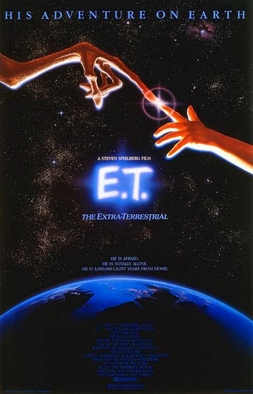
\includegraphics[height=.7\textheight]{et}\\
            {\tiny (Image: John Alvin, (c) 1982 Universal Studios)}
        \end{column}
    \end{columns}

    \vfill

    \footnotesize \ftnt{\cf{} fermions: if $\psi$ obeys $(\mathrm{i}\slashed\partial-m)\psi=0$, then $(\operatorname{CP}\psi)$ is also a solution (\textbf{C}harge and \textbf{P}arity inverted)}
\end{frame}

\begin{frame}{On the other hand\ldots}
    \begin{columns}[T]
        \begin{column}{.6\textwidth}
            \begin{itemize}
				\item Baryon asymmetry of the Universe:
                \begin{equation*}
                    \mathcal{O}(\eta_\text{cosm}) = \mathcal{O} \! \left( \frac{n_B - n_{\overline{B}}}{n_\gamma} \right) \sim 10^{-10} \neq 0,
                \end{equation*}
                with $n_{B,\overline{B},\gamma}=$ number of baryons, anti-baryons and photons
                \item Universe is filled with matter (rather than anti-matter\ftnt)
                \item Standard Model of Cosmology: Big Bang produces $n_B = n_{\overline{B}}$~~(\textbf{CP invariant})
                \item Evolution: QED and QCD are \textbf{CP invariant}
            \end{itemize}
        \end{column}
        \begin{column}{.4\textwidth}
        \end{column}
    \end{columns}

    \vspace{5mm}
    \footnotesize \ftnt{} \textit{i.e.}, most likely alien world is made out of matter as well
\end{frame}

\begin{frame}{Introduction}
    \begin{columns}[T]
        \begin{column}{.6\textwidth}
			\scalebox{1.2}{Can we explain $\mathcal{O}(\eta_\text{cosm})$?}
            \begin{itemize}
                \item \textbf{No!} We fail to describe one of the most obvious property of our Universe!
            \end{itemize}
            Can we (at least) describe some CP violating processes?
            \begin{itemize}
                \item Yes! The Standard Model of Particle Physics contains a CP violating sector (weak interaction)
                \item However, it does not predict the right order of magnitude of $\eta_\text{cosm}$\,!
            \end{itemize}
        \end{column}
        \begin{column}{.4\textwidth}
            \centering
            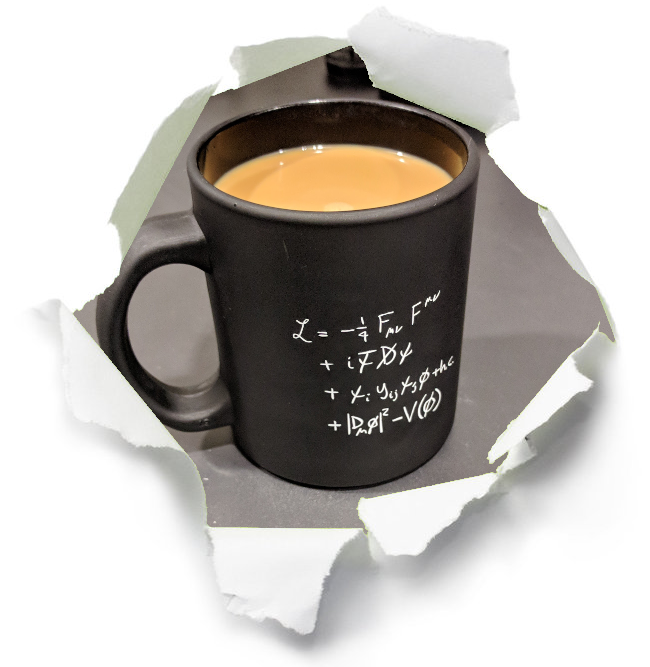
\includegraphics[height=.7\textheight]{cup}
        \end{column}
    \end{columns}
\end{frame}

\begin{frame}{Introduction}
    \begin{itemize}
        \item Diagonalizing Yukawa matrices\ftnt{} leads to \textbf{quark \textcolor{vertexDarkRed}{mass} eigenstates} $q$, but skews \textbf{quark \textcolor{vertexDarkRed}{flavor} eigenstates} $q'$
        \begin{equation*}
            \mathcal{J}^\mu_{\!cc} \; \supset \;
            (\overline{u'},\, \overline{c'},\, \overline{t'}) \, \gamma^\mu \frac{1-\gamma^5}{2} \begin{pmatrix}d' \\ s' \\ b' \end{pmatrix}
            \quad \longrightarrow \quad
            (\overline{u},\, \overline{c},\, \overline{t}) \, \gamma^\mu \frac{1-\gamma^5}{2} V_\text{\!CKM} \begin{pmatrix}d \\ s \\ b \end{pmatrix}
        \end{equation*}
        \begin{center}
            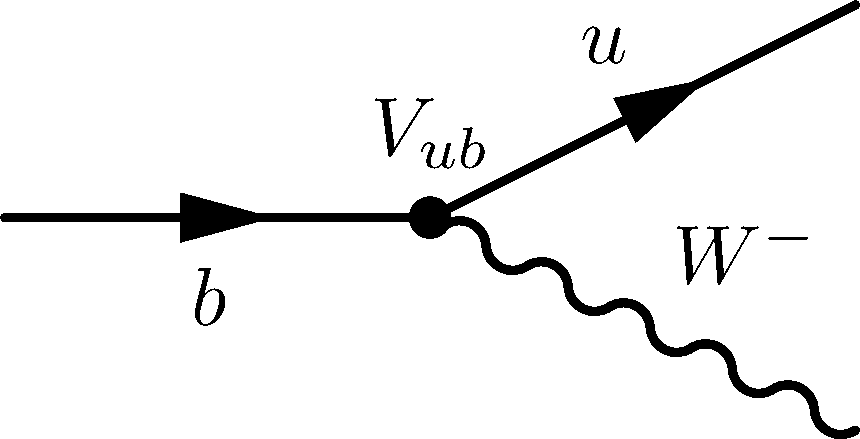
\includegraphics[width=.2\textwidth,valign=c]{decay_b2u}
            \scalebox{1.5}{\;+\;}
            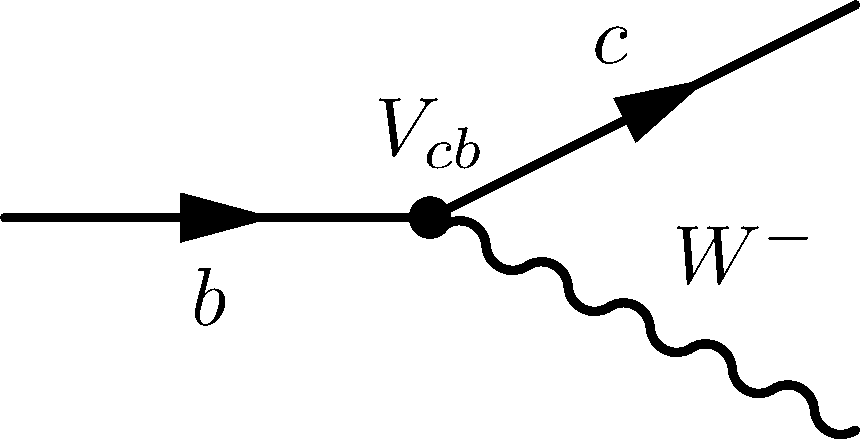
\includegraphics[width=.2\textwidth,valign=c]{decay_b2c}
            \scalebox{1.5}{\;+\;}
            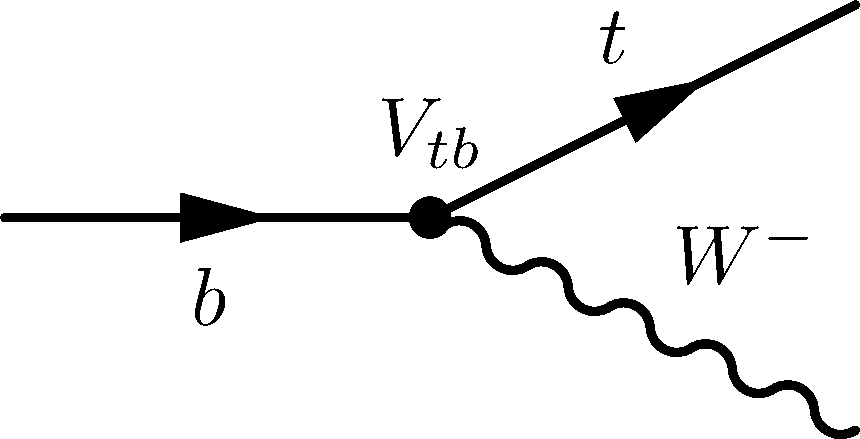
\includegraphics[width=.2\textwidth,valign=c]{decay_b2t}
        \end{center}
        \vspace{1em}
        \item This introduces the non-trivial transformation matrix $V_\text{CKM}$ for quarks (CKM matrix)
        \item $V_\text{CKM}$ is a \textbf{unitary} $3 \times 3$ matrix (CP violation \textit{in} complex phases)
    \end{itemize}

    \vspace{5mm}
    \footnotesize \ftnt{}\textit{cf.} Higgs mechanism
\end{frame}

\begin{frame}{State-of-the-art}
    \textbf{What we know}
    \begin{itemize}
        \item We understand CP violation (CPV) on quark level in the framework of the Standard Model (SM)
        \item CPV is predicted and confirmed with high confidence for \textbf{mesons}\ftnt{} at particle accelerators
    \end{itemize}
    \textbf{What we don't know}
    \begin{itemize}
        \item Absence of anti-\textbf{baryons}\ftnt{} is a large scale CPV which we cannot explain
        \item (strong CPV, neutrino CPV, Sakharov conditions, \ldots)
    \end{itemize}

    \textbf{Idea of this analysis}
    \begin{itemize}
        \item Establish (yet unknown) \textbf{baryon} decay which can be used (in the future) to measure CPV parameter of the SM
    \end{itemize}

    \vfill

    \footnotesize\ftnt meson / anti-meson: $(\quark\quarkbar)$, baryon: $(\quark\quark\quark)$, anti-baryon: $(\quarkbar\quarkbar\quarkbar)$
\end{frame}

\begin{frame}{The decay \decay{\Lb}{\Dz\Lz}}
    \begin{columns}[T]
        \begin{column}{.45\textwidth}
            \centering
            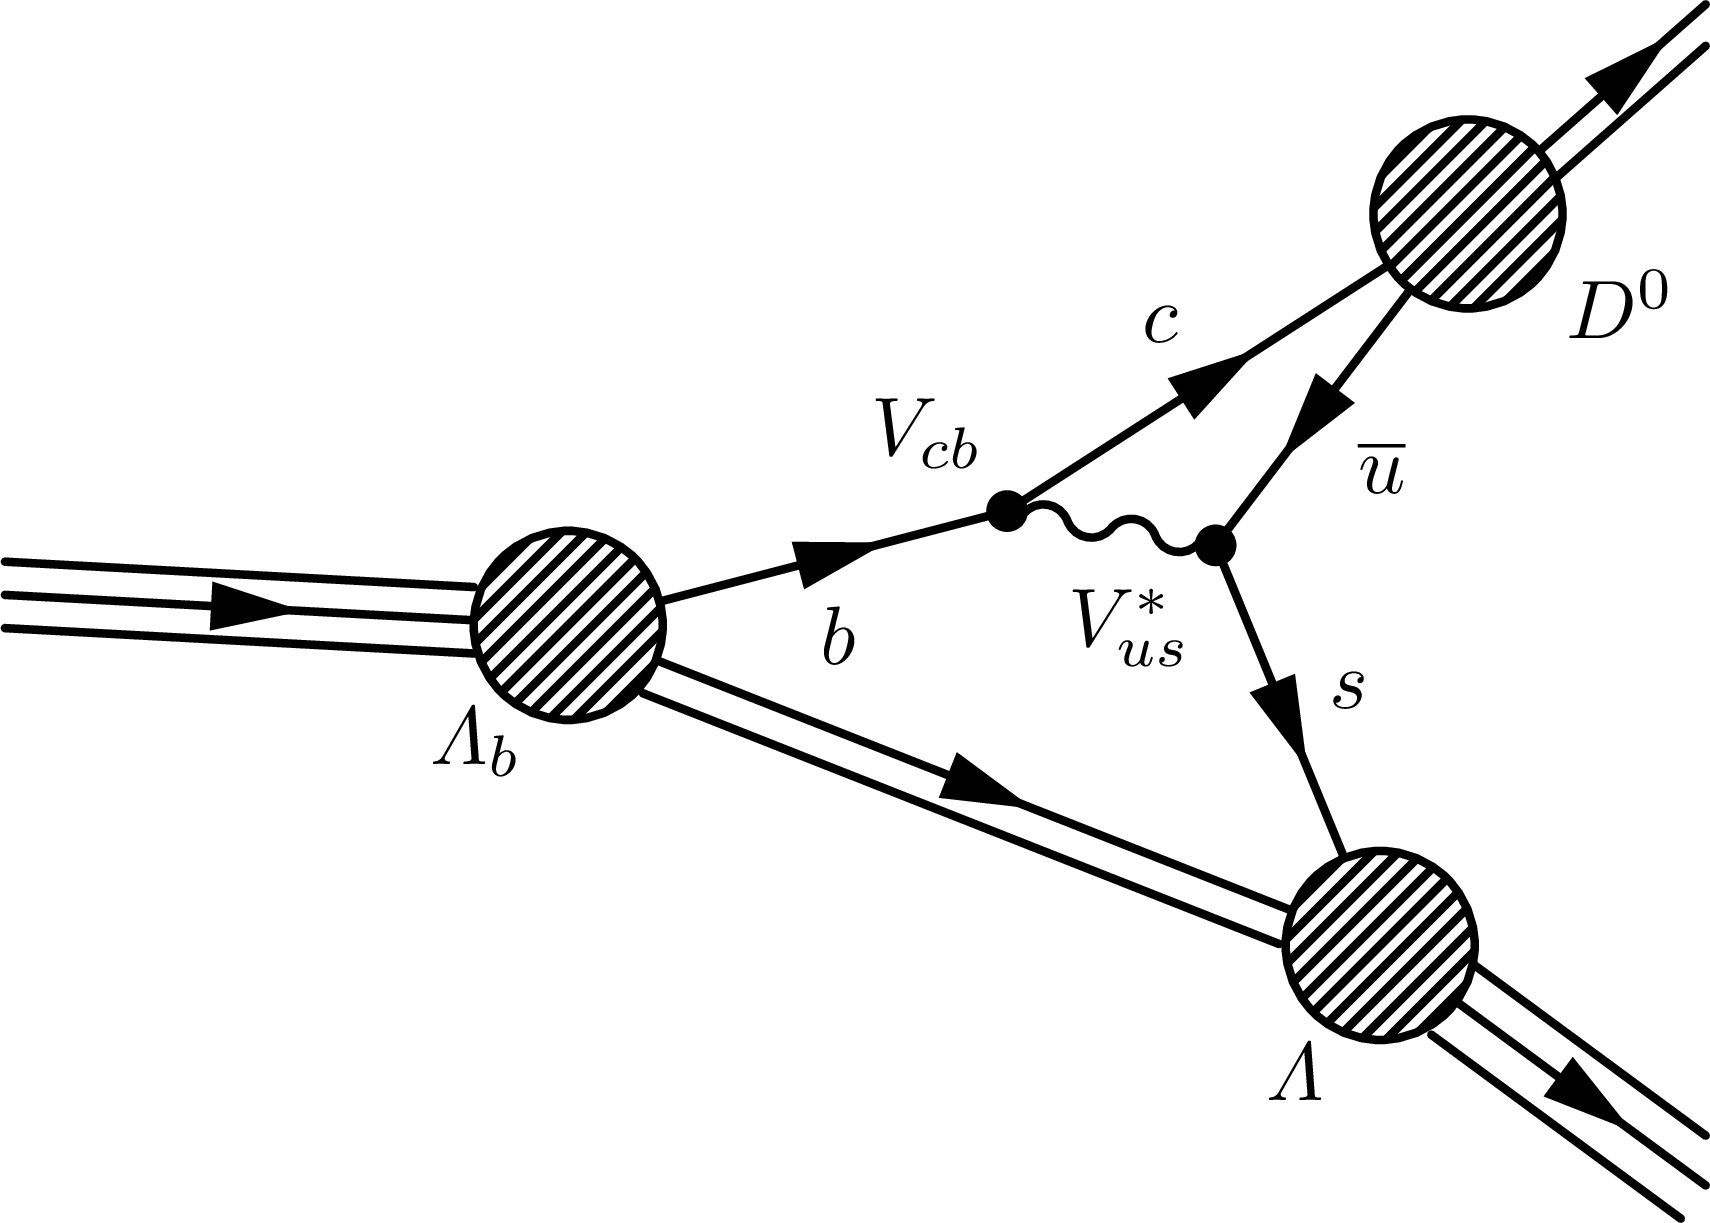
\includegraphics[height=.5\textheight]{misc/decayLb2DzLz}
        \end{column}
        \begin{column}{.45\textwidth}
            \centering
            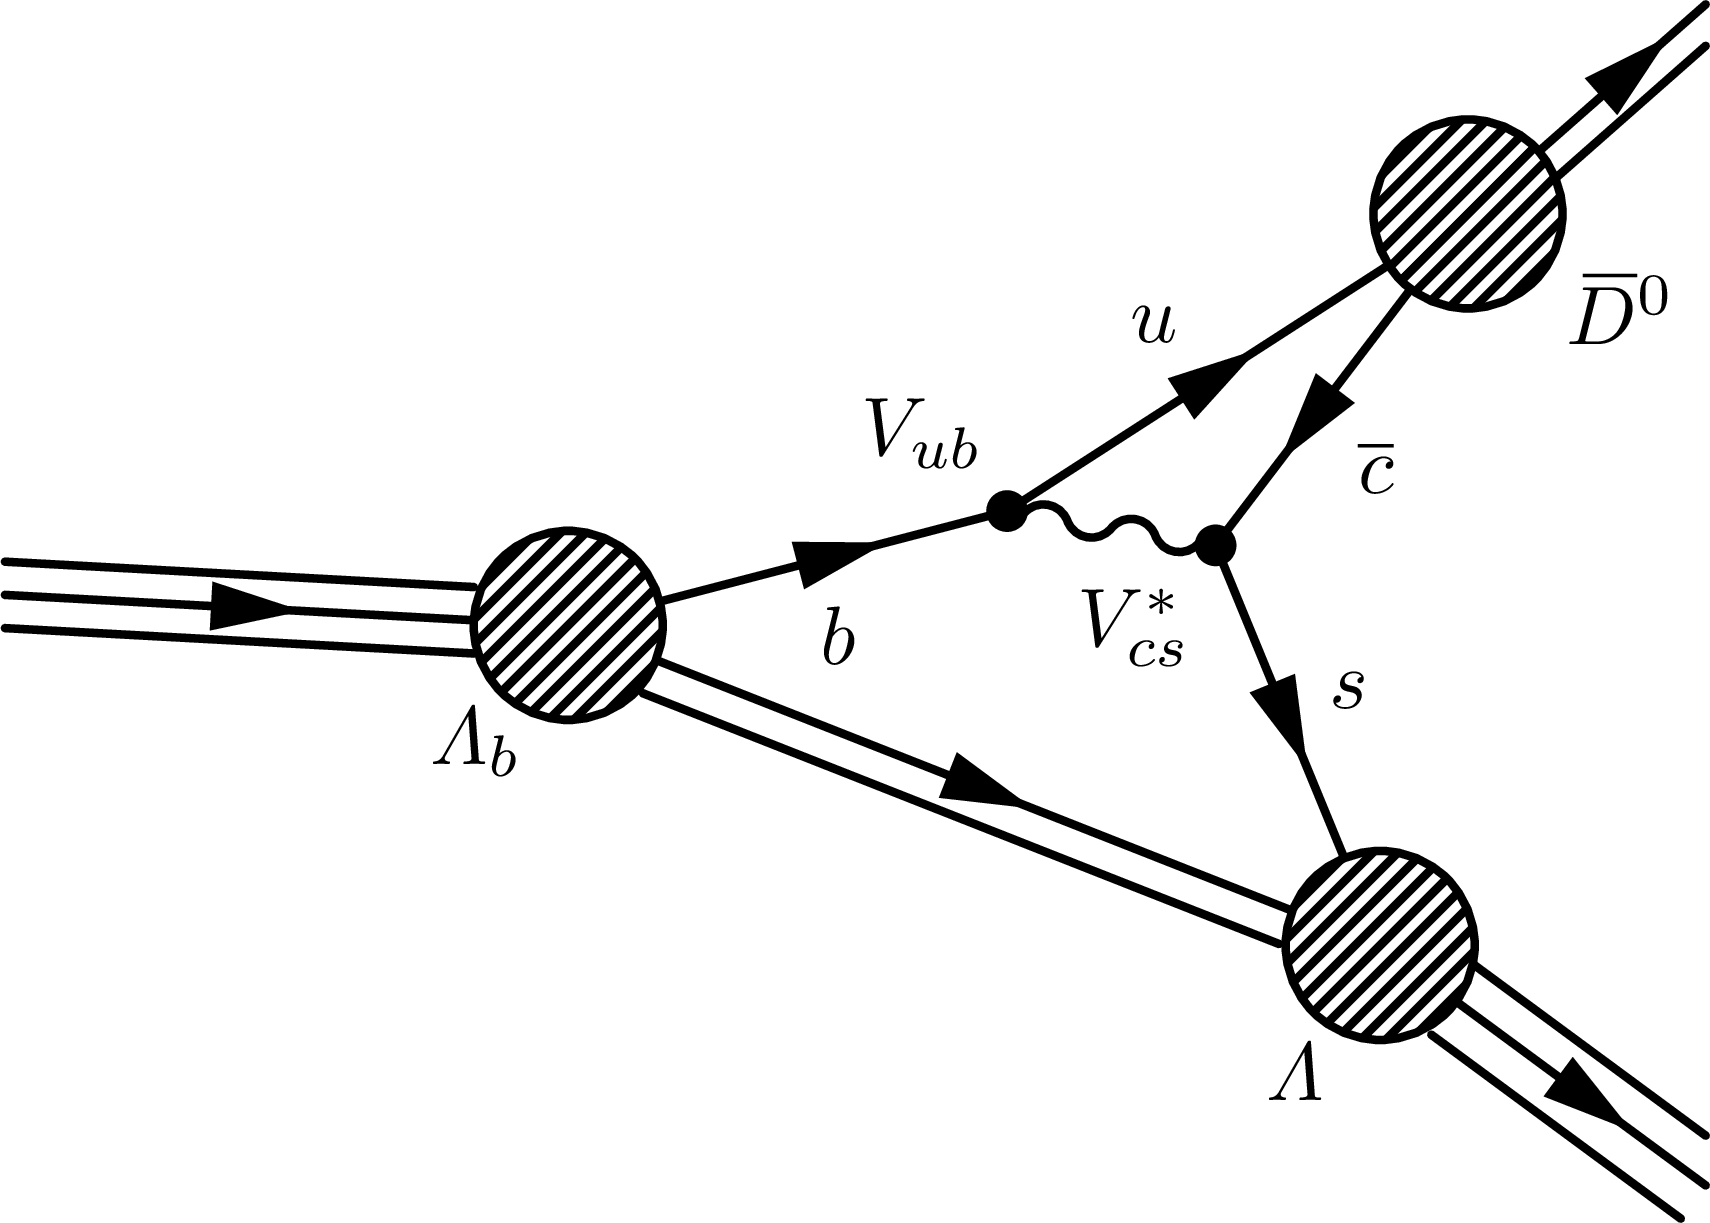
\includegraphics[height=.5\textheight]{misc/decayLb2DzbLz}
        \end{column}
    \end{columns}

    \begin{itemize}
        \item Perfectly suited for LHCb
        \item CKM angle: $\gamma + \mathcal{O}(\lambda^4)$ (without CPV in \Dz system)
        \item CPV in \decay{\Lb}{\Dz/\Dzb\Lz} and
        \begin{itemize}
            \item $\decay{\Dz/\Dzb}{\Kp\pim}$ (CPV but Cabibbo suppressed, \textbf{future prospect})
            \item $\decay{\Dz/\Dzb}{\Kp\Km \,/\, \pip\pim}$ (CPV but Cabibbo suppressed, \textbf{future prospect})
            \item $\decay{\Dz}{\Km\pip}$ (no CPV but Cabibbo favored, \textcolor{vertexDarkRed}{\textbf{this analysis}})
        \end{itemize}
    \end{itemize}
\end{frame}

\begin{frame}{Large Hadron Collider}
    \centering
    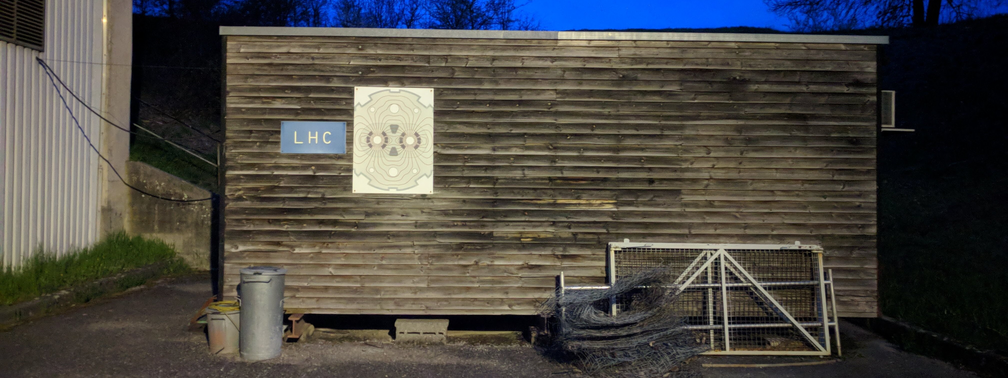
\includegraphics[height=.6\textheight]{lhc}\\
    \vspace{-2mm}
    \begin{center}
        \footnotesize (Symbolic image, picture taken at CERN site)
    \end{center}

    \begin{columns}[T]
        \begin{column}{.45\textwidth}
            \begin{itemize}
                \item World's largest and highest-energy particle accelerator 
                \item Built by CERN
            \end{itemize}
        \end{column}
        \begin{column}{.55\textwidth}
            \begin{itemize}
                \item Collides proton beams with $\sqrt{s}=13\,$TeV
                \item \bquark baryon factory (\Lb is lightest \bquark baryon)
            \end{itemize}
        \end{column}
    \end{columns}
\end{frame}

\begin{frame}{LHCb Experiment}
    \centering
    \enquote{LHCb is an experiment set up to explore what happened after the Big Bang that allowed matter to survive and build the Universe we inhabit today}

    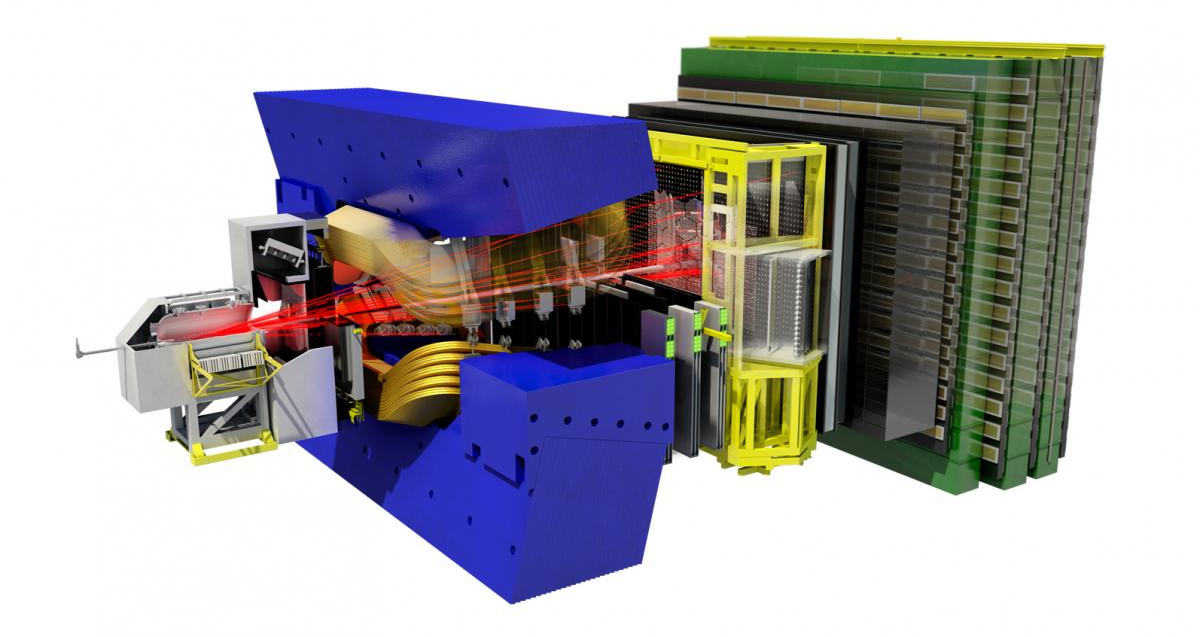
\includegraphics[height=.5\textheight]{detector}
    \begin{columns}[T]
        \begin{column}{.5\textwidth}
            \begin{itemize}
                \item One of the four major experiments at the LHC
                \item Dataset: $6\,\text{fb}^{-1}$ at $\sqrt{s}=13\,$TeV
            \end{itemize}
        \end{column}
        \begin{column}{.5\textwidth}
            \textbf{Multipurpose detector}, \eg{}:
            \begin{itemize}
                \item Excellent vertex resolution
                \item Powerful particle identification
            \end{itemize}
        \end{column}
    \end{columns}
\end{frame}

\begin{frame}{Outline}
    \scalebox{1.2}{\textbf{Why / What?}}
    \begin{itemize}
        \item Pave the way to measure CPV in decays of baryons at colliders
        \item Prose: search for the decays $$\decay{\Lb/\Xibz}{[\Km\pip]_{\Dz} \, [\proton\pim]_{\Lz}}$$
    \end{itemize}

    \scalebox{1.2}{\textbf{How?}}
    \begin{itemize}
        \item (Data calibration and pre-processing\ftntdagger)
        \item Classification of data as \textit{signal} and \textit{background} using MVA\ftntasterix
        \item (Study various physical backgrounds\ftntdagger)
        \item Count signal events with fit and estimate stat.\ significances\ftntasterix
        \item Estimate branching ratios $\mathcal{B}(\decay{\Lb}{\Dz\Lz})/\mathcal{B}(\decay{\Lb}{\Dz\proton\pim})$\ftntdagger{} and $\mathcal{B}(\decay{\Xibz}{\Dz\Lz})/\mathcal{B}(\decay{\Lb}{\Dz\Lz})$\ftntasterix
    \end{itemize}

    \footnotesize
    \ftntdagger not discussed here, \ftntasterix partially discussed here
\end{frame}

\begin{frame}{How to find genuine decays? \textemdash Example \decay{\Lz}{\proton\pim}}
    \begin{columns}
        \begin{column}{.55\textwidth}
            \begin{itemize}
                \item Create \Lz candidates: $\{\Lz\} := \{\proton\} \otimes \{\pim\}$
                \item Use inv.\ mass $m(\Lz)\ftnt{} \overset{?}{=} m(\proton\pim)$ as proxy
                \item Separate components:
                \begin{enumerate}
                    \item Combinatorial background \\ \scalebox{.8}{(random track combinations)}
                    \item physical background \\ \scalebox{.8}{(\eg{}, \decay{\KS}{\textcolor{vertexDarkRed}{\pip}\pim})}
                    \item genuine \decay{\Lz}{\proton\pim} decays
                \end{enumerate}
            \end{itemize}
        \end{column}
        \begin{column}{.45\textwidth}
            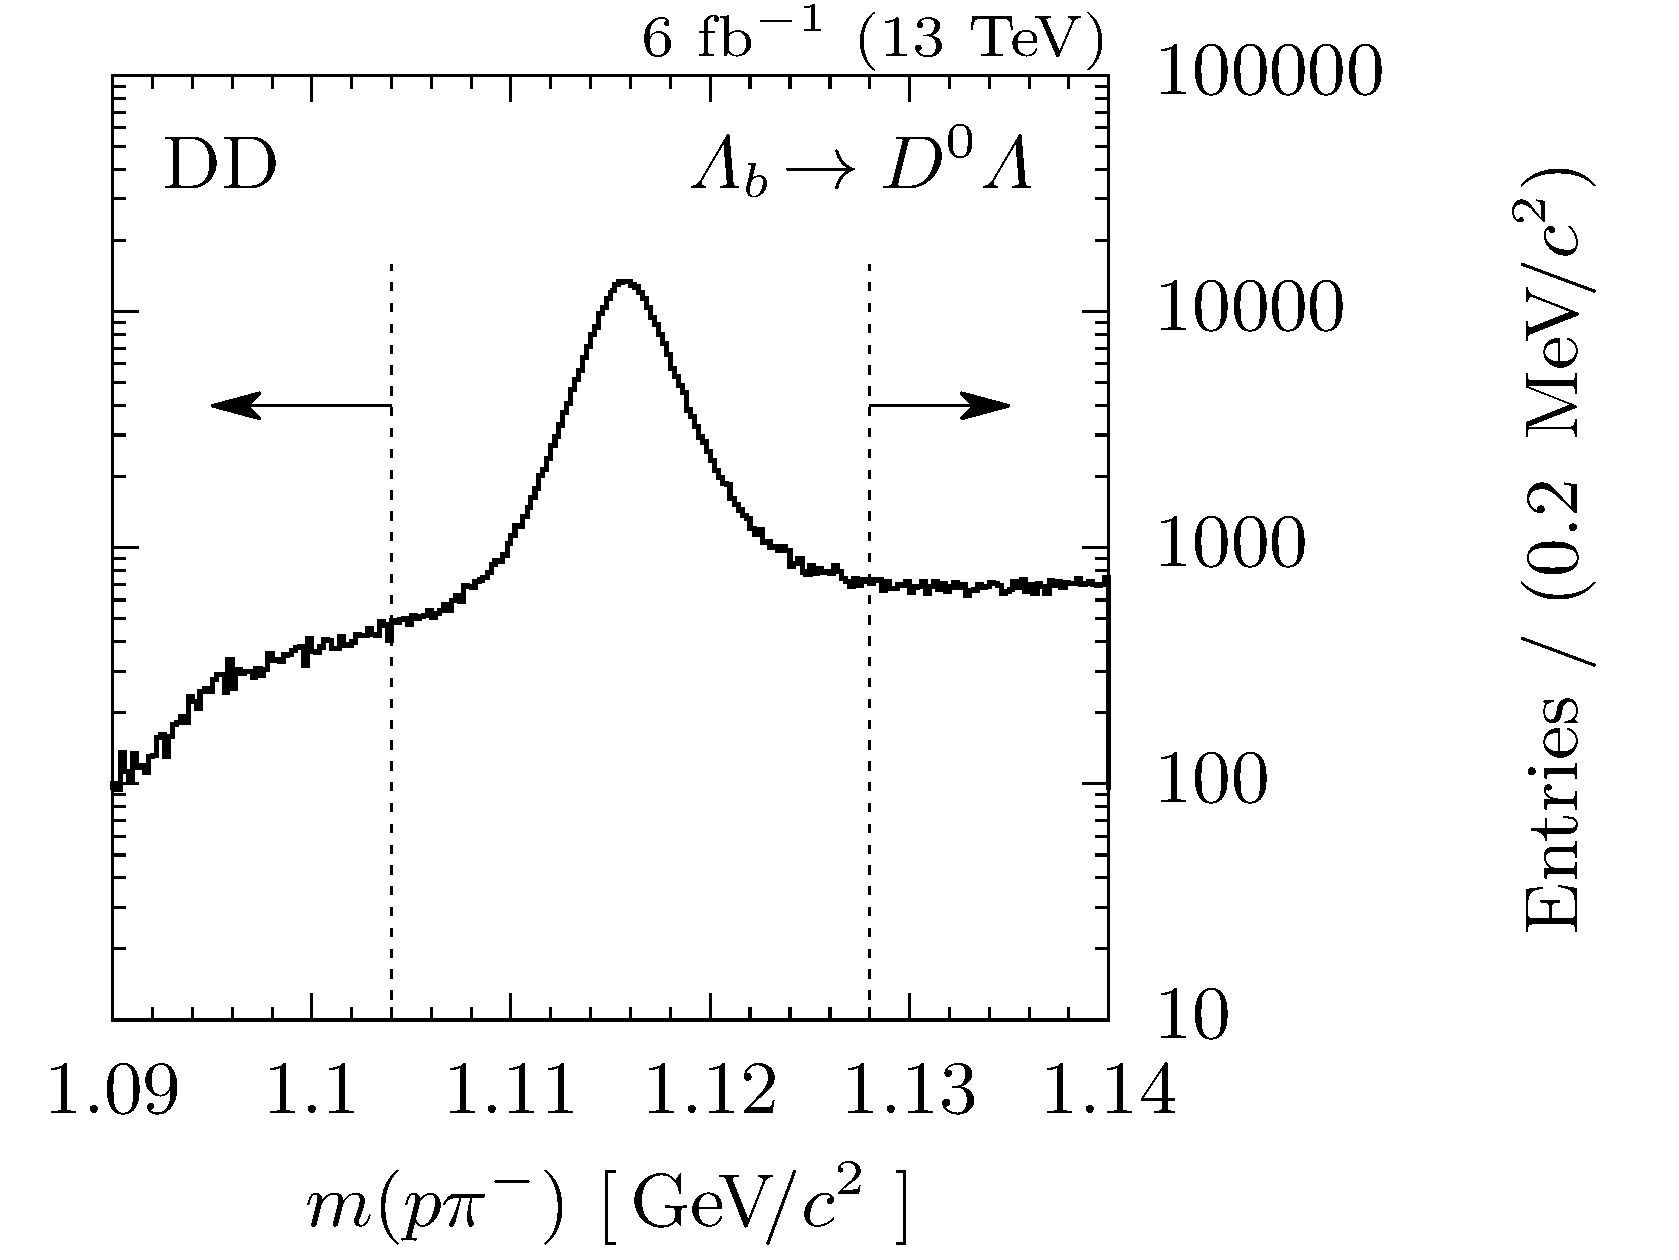
\includegraphics[width=\textwidth]{mvaLz/hLzM_DD}\\
            \hspace{5mm} \footnotesize (\ftnt PDG: $m(\Lz) \approx 1.117\gevcc$)
        \end{column}
    \end{columns}

    \vspace{5mm}

    \scalebox{0.8}{\vbox{%
    Technical detail: only (weak) Cabibbo suppressed decays possible for \Lz
    \vspace{-2mm}
    \begin{itemize}
        \item \textit{long} lifetime
        \item some \Lz decay outside (inside) of first detector element: refer to as \textbf{DD} (\textbf{LL})
        \item different detector response, separate analysis necessary
    \end{itemize}}}
\end{frame}

\begin{frame}[plain,noframenumbering]
    \centering
    \scalebox{2.}{Do the same for \decay{\Lb/\Xibz}{\Dz\Lz}?}

    \ie{}, $\{ \Lb/\Xibz \} := \underbrace{\{ \Km \} \otimes \{ \pip \}}_{\{ \Dz \}} \otimes \underbrace{\{ \proton \} \otimes \{ \pim \}}_{\{ \Lz \}}$
\end{frame}

\begin{frame}{Searching for \decay{\Lb/\Xibz}{\Dz\Lz}}
    \begin{columns}
        \begin{column}{.55\textwidth}
            \textbf{No signal visible!}
            \begin{itemize}
                \item Background (at this stage) mainly combinatorial
                \item Need to increase
                \begin{itemize}
                    \item purity of $\{ \Dz \}$
                    \item purity of $\{ \Lz \}$
                    \item filter $\{ \Dz \} \otimes \{ \Lz \}$ for $\decay{\Lb/\Xibz}{\Dz\Lz}$ decays by constraining physical properties
                \end{itemize}
                \item (Carefully analyse physical backgrounds\ftntdagger)
            \end{itemize}
        \end{column}
        \begin{column}{.45\textwidth}
            \only<1>{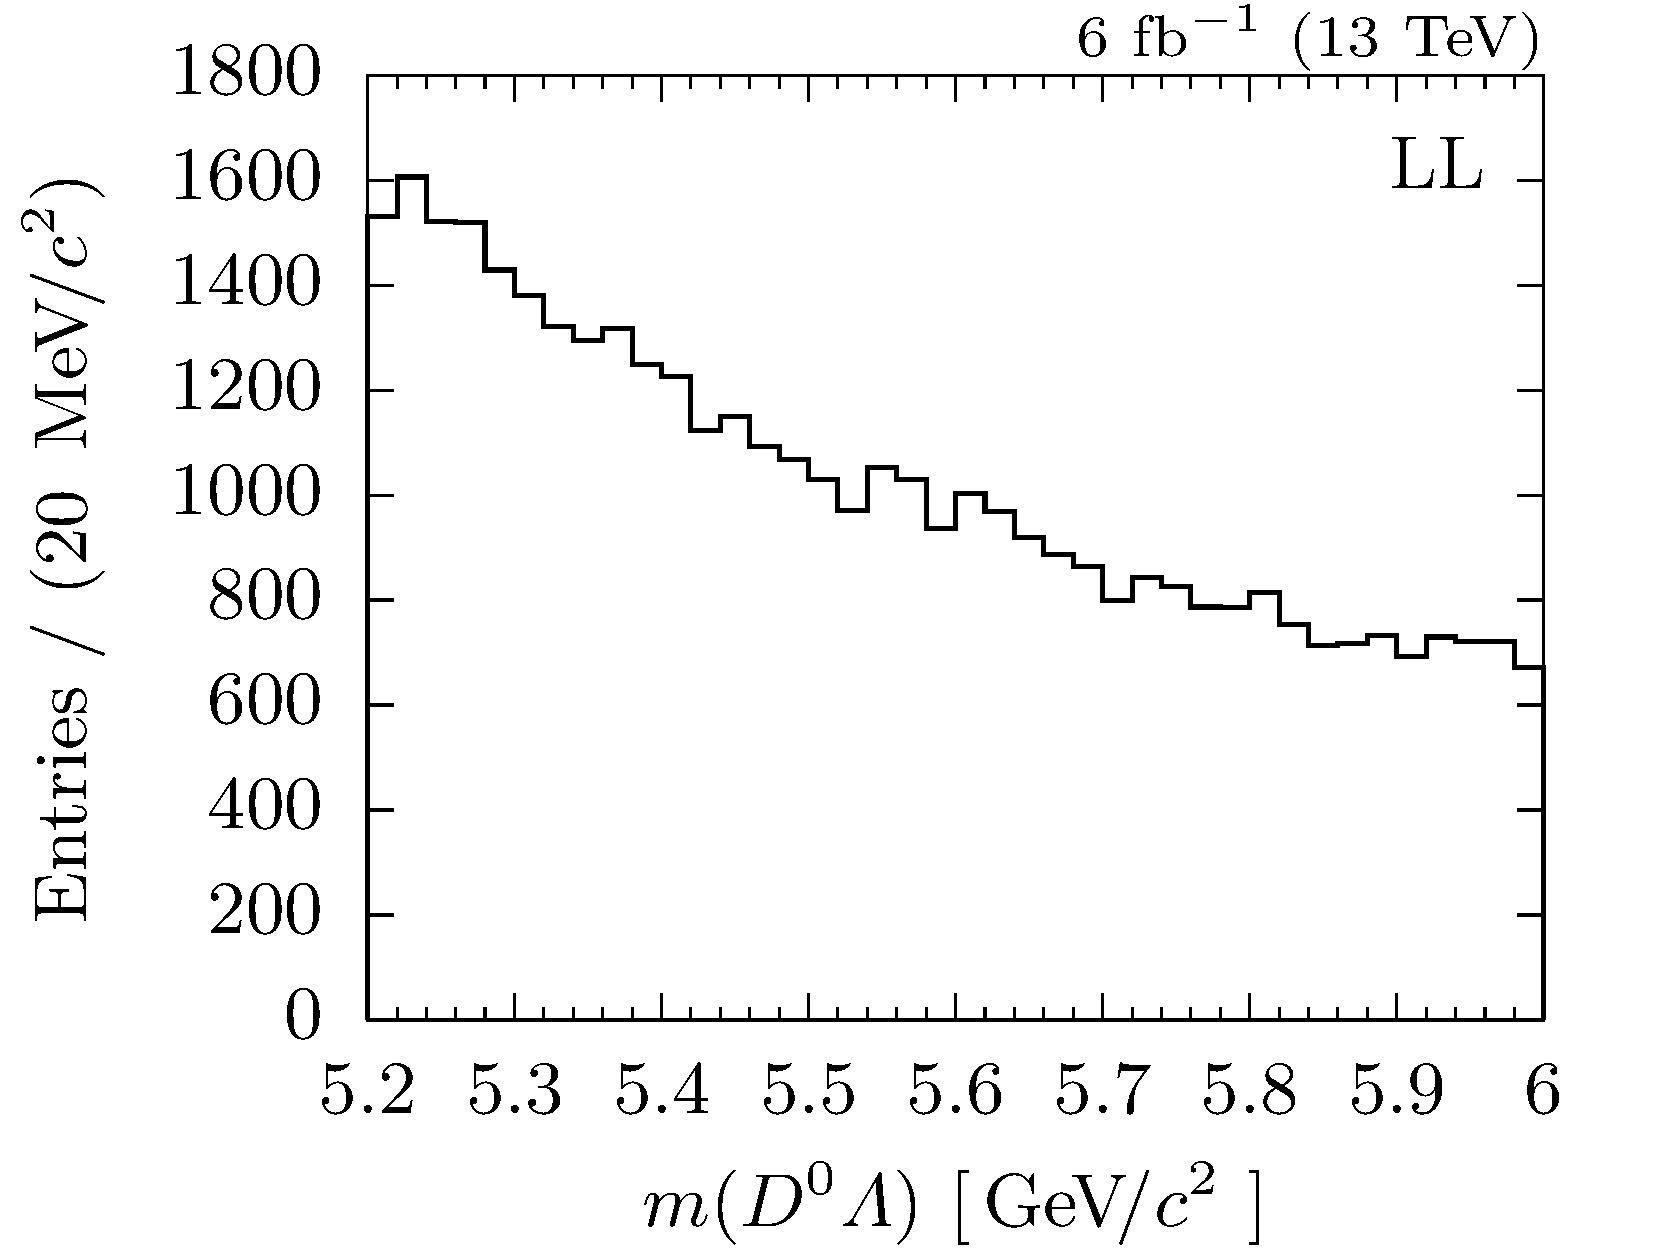
\includegraphics[width=\textwidth]{mvaLbDz/hDzLzM_LL}}%
            \only<2>{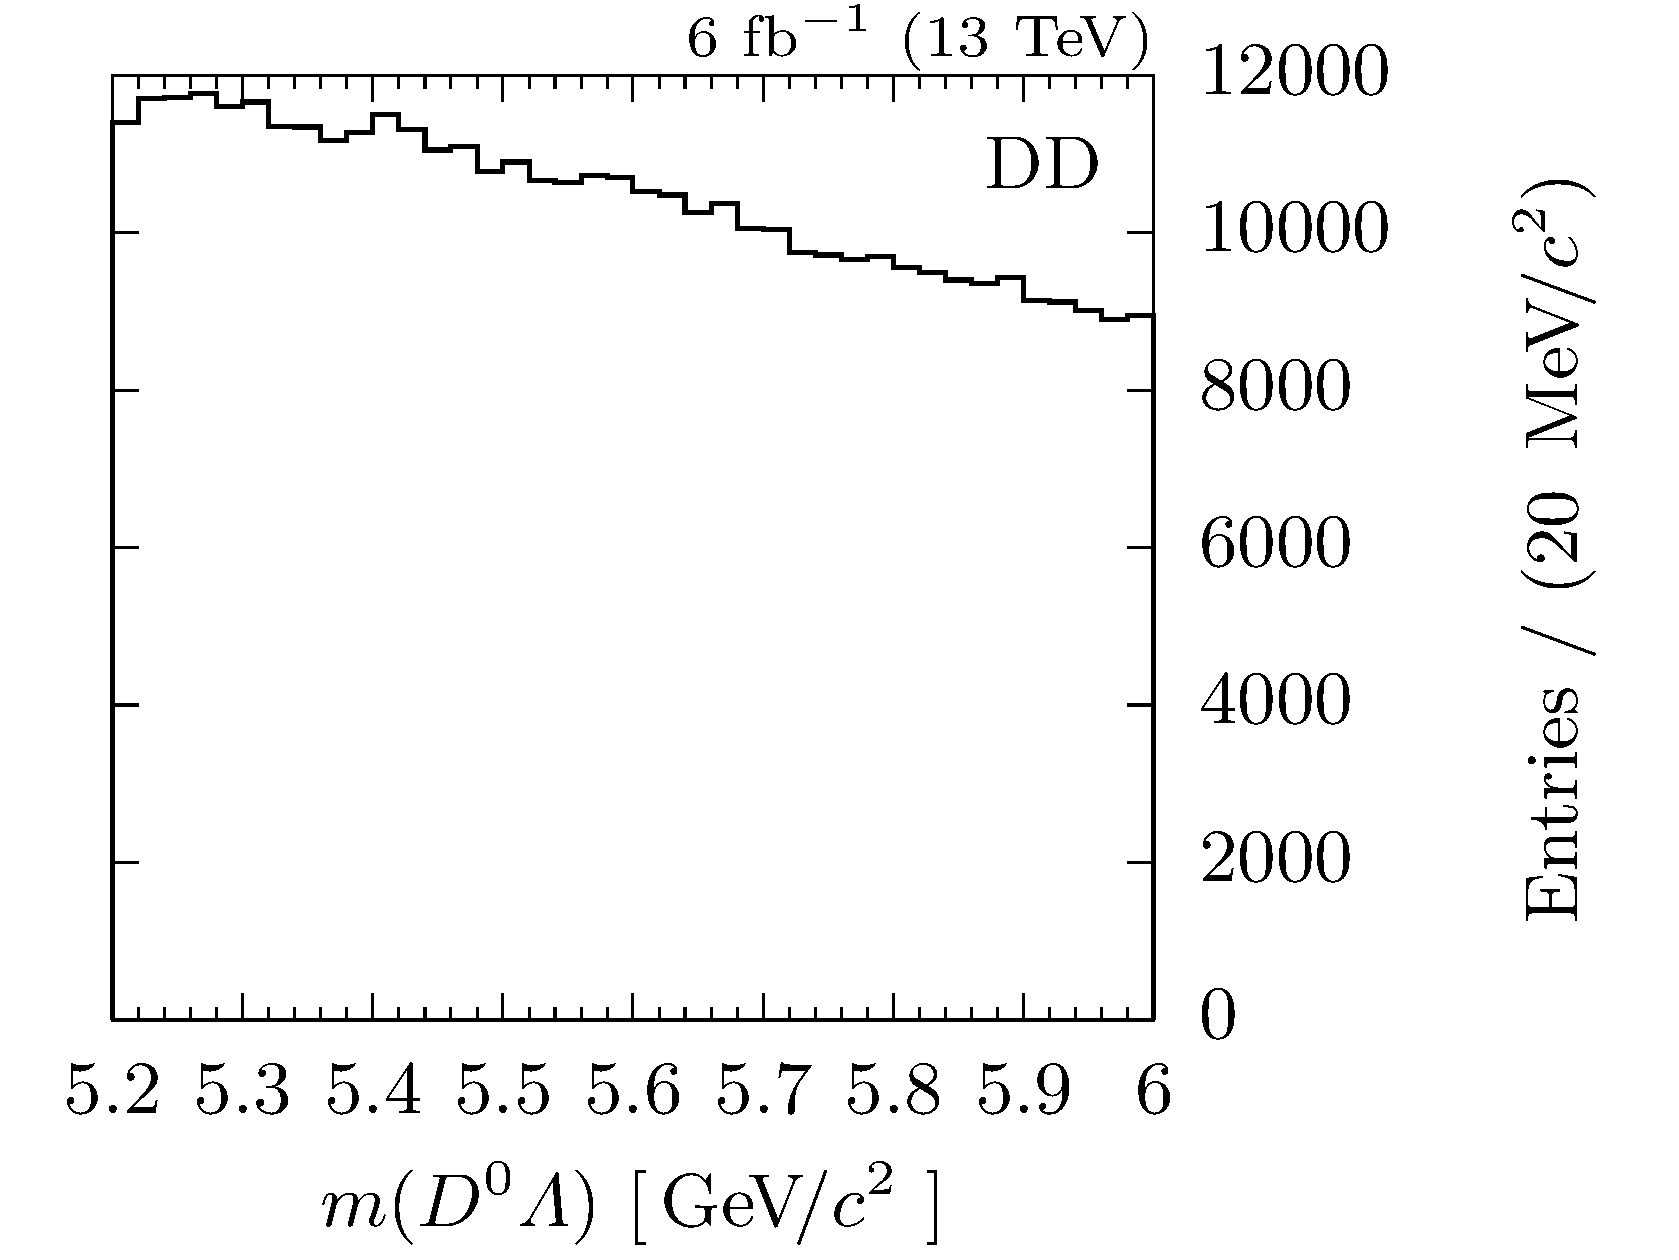
\includegraphics[width=\textwidth]{mvaLbDz/hDzLzM_DD}}%
            \\
            \hspace{5mm} \footnotesize (PDG: $m(\Lb) \approx 5.620\gevcc$,\\
            \hspace{5mm} \footnotesize \phantom{(}PDG: $m(\Xibz) \approx 5.792\gevcc$)
        \end{column}
    \end{columns}
\end{frame}

\begin{frame}{Searching for \decay{\Lb/\Xibz}{\Dz\Lz}}
    \begin{columns}
        \begin{column}{.6\textwidth}
            \textbf{Use ML to rescue!} Classification problem
            \begin{itemize}
                \item Separate \textit{\textbf{signal}} (genuine \decay{\Lb/\Xibz}{\Dz\Lz})
                \item \ldots from (combinatorial) \textit{\textbf{background}}
                \item Labels?
                \begin{itemize}
                    \item use MC simulated decays for class \textit{signal}\ftntdagger{}
                    \item use recorded data from sidebands for class \textit{background}
                \end{itemize}
            \end{itemize}
        \end{column}
        \begin{column}{.4\textwidth}
            \centering
            
\includegraphics[width=.5\textwidth]{needle_haystack}\\
            {\tiny (Image: R.~Diepenheim on \texttt{thenounproject.com})}
        \end{column}
    \end{columns}

    \vspace{5mm}

    \footnotesize \ftntdagger{} calibration needed (not discussed here)
\end{frame}

\begin{frame}{MVA methodoloy}
    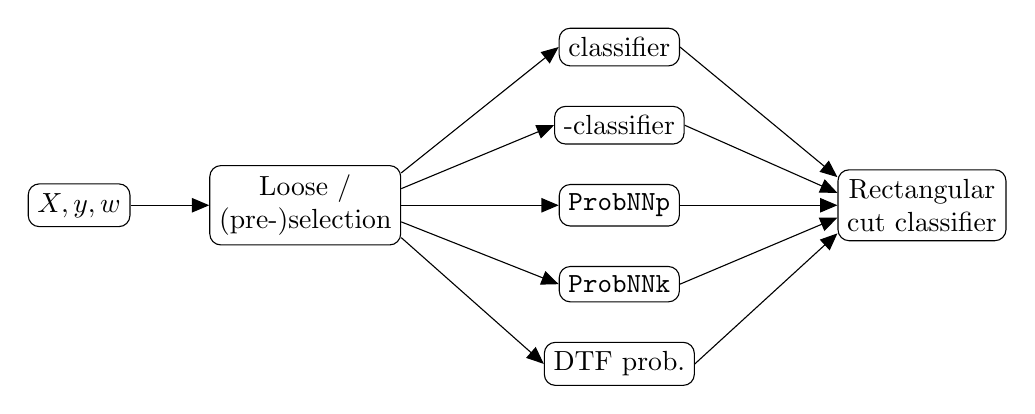
\begin{tikzpicture}[>=triangle 45,
                        node/.style={rectangle,align=center,rounded corners}]
        \node[draw,node] (data) {$X, y, w$};
        \node[draw,node,right=1cm of data] (presel) {Loose / \\ (pre-)selection\ftntdagger};
        \node[draw,node,right=2cm of presel] (pProbNNp) {\texttt{ProbNNp}\ftnt{}};
        \node[draw,node,above=.5cm of pProbNNp] (clfLbDz) {\Lb-\Dz classifier};
        \node[draw,node,above=.5cm of clfLbDz] (clfLz) {\Lz classifier};
        \node[draw,node,below=.5cm of pProbNNp] (kProbNNk) {\texttt{ProbNNk}\ftnt{}};
        \node[draw,node,below=.5cm of kProbNNk] (dtf) {DTF prob.};
        \node[draw,node,right=2cm of pProbNNp] (fclf) {Rectangular\\ cut classifier};

        \draw[->] (data) -- (presel);
        \draw[->] (presel) -- (pProbNNp);
        \draw[->] (presel.north east) + (0,-1mm) -- (clfLz.west);
        \draw[->] (presel.north east) + (0,-3mm) -- (clfLbDz.west);
        \draw[->] (presel.south east) + (0, 3mm) -- (kProbNNk.west);
        \draw[->] (presel.south east) + (0, 1mm) -- (dtf.west);
        \draw[->] (pProbNNp) -- (fclf);
        \draw[->] (clfLz.east) -- ($(fclf.north west) + (0,-1mm)$);
        \draw[->] (clfLbDz.east) -- ($(fclf.north west) + (0,-3mm)$);
        \draw[->] (kProbNNk.east) -- ($(fclf.south west) + (0,3mm)$);
        \draw[->] (dtf.east) -- ($(fclf.south west) + (0,1mm)$);
    \end{tikzpicture}

    \textbf{Training:} classify $m$ data $X \in \mathbb{R}^{m \times n}$ with $n$ features using labels $y \in \{ \text{sig.}, \text{bkg.} \}^m$ and calibration factors\ftntdagger{} $w \in \mathbb{R}^m$ with $\mathcal{O}(m) = 10k$, $n = 18$

    \vspace{5mm}
    \footnotesize \ftnt{} pre-trained shallow NN
\end{frame}

\begin{frame}{Example: \Lz classifier}
    \begin{columns}
        \begin{column}{.55\textwidth}
            \begin{itemize}
                \item 5 features of $\{ \Lz \}$: 
                \begin{enumerate}
                    \item transverse momentum
                    \item angle between momentum and connecting line between \proton\proton-IA point (PV) and \Lz decay vertex
                    \item $\chi^2$ improvement of PV with \Lz track
                    \item fit prob.\ of decay vertex
                    \item significance of flight distance
                \end{enumerate}
                \item Separate classifiers for LL and DD
                \item Optimize hyper-parameters of 5 classifiers using grid search w.r.t.\ ROC-AUC\ftnt{} value
            \end{itemize}
        \end{column}
        \begin{column}{.45\textwidth}
            \centering
            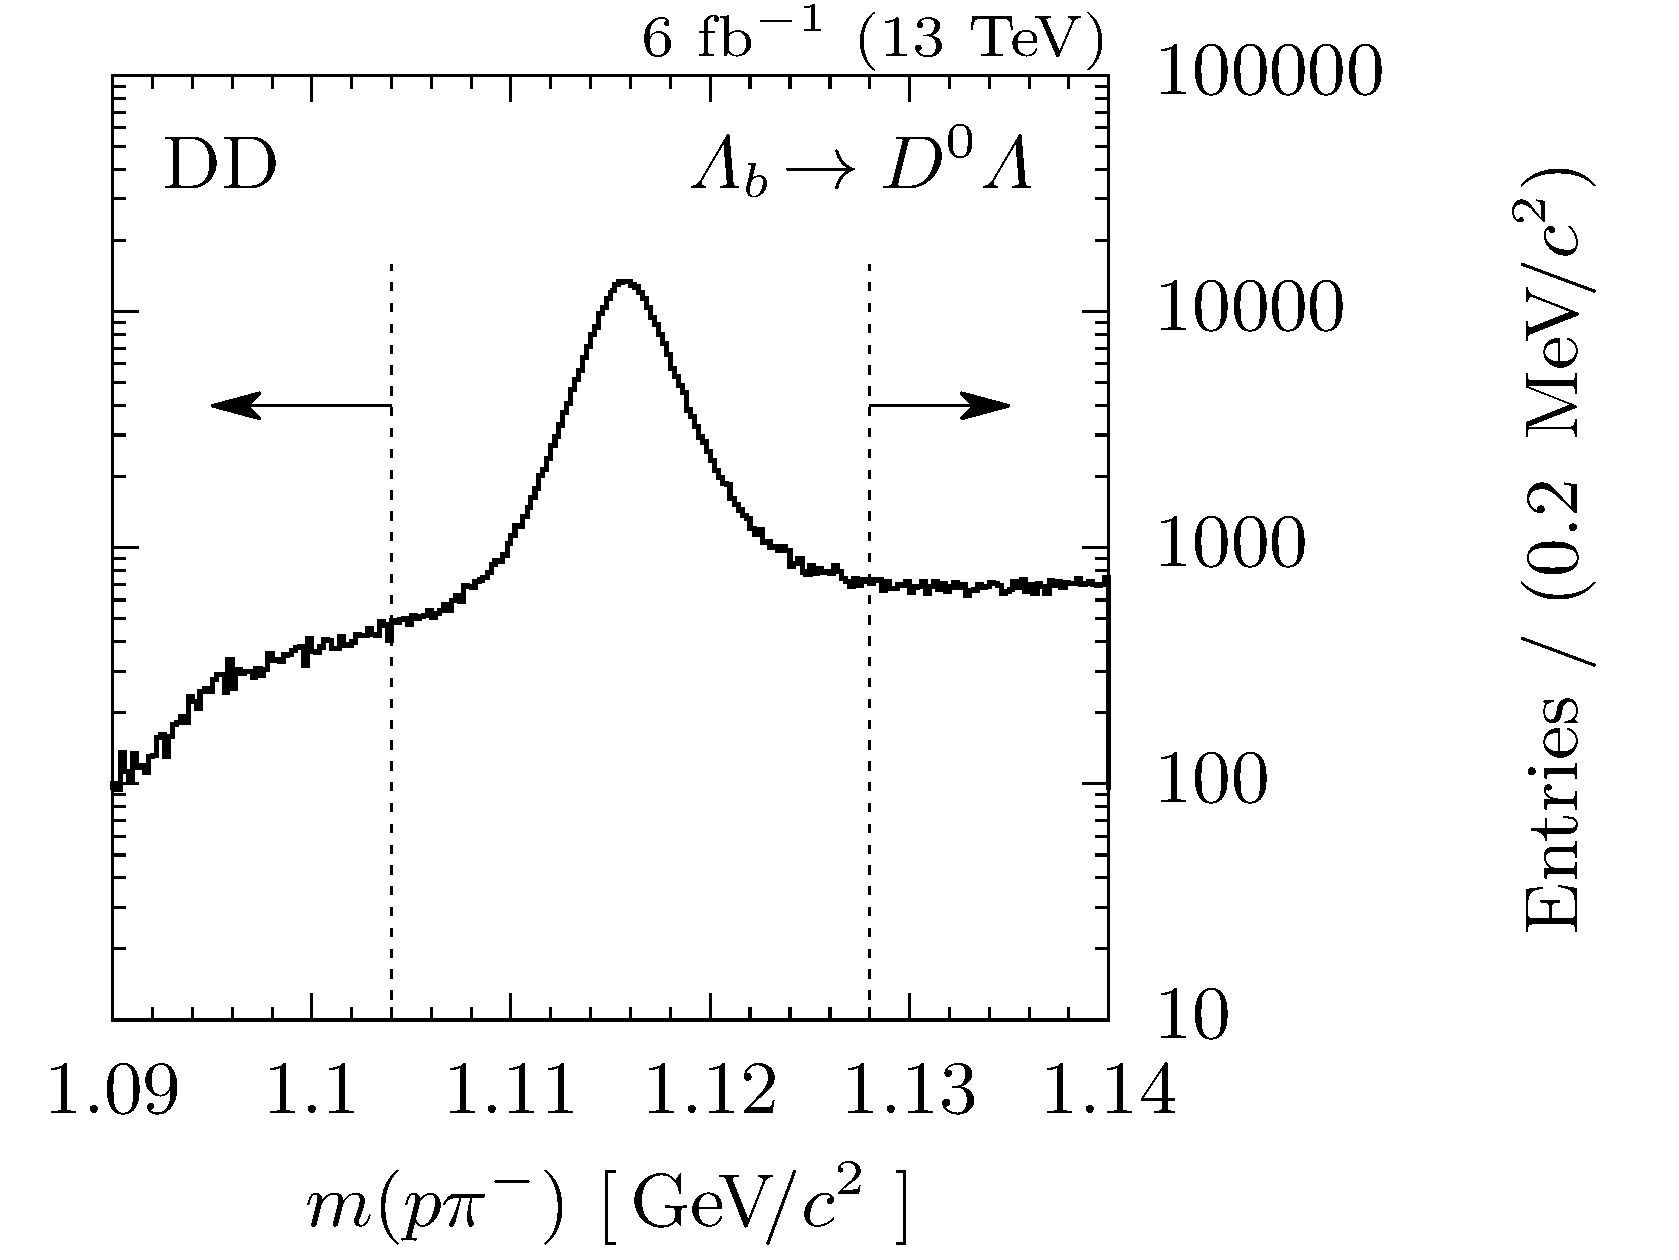
\includegraphics[scale=1.]{mvaLz/hLzM_DD}
        \end{column}
    \end{columns}

    \vspace{5mm}
    \footnotesize \ftnt{} Prob.\ that clf.\ will rank randomly chosen \textit{sig.} instance higher than randomly chosen \textit{bkg.} one
\end{frame}

\begin{frame}{Example: \Lz classifier}
    \begin{columns}
        \begin{column}{.45\textwidth}
            \scalebox{1.2}{\Lz classifier}
            \begin{itemize}
                \item \textcolor{vertexDarkRed}{5 features of $\{ \Lz \}$}
                \item Separate classifiers for LL and \textbf{DD}
                \item Optimize hyper-parameters of 5 classifiers using grid search w.r.t.\ ROC-AUC\ftnt{} value
            \end{itemize}
        \end{column}
        \begin{column}{.5\textwidth}
            \centering
            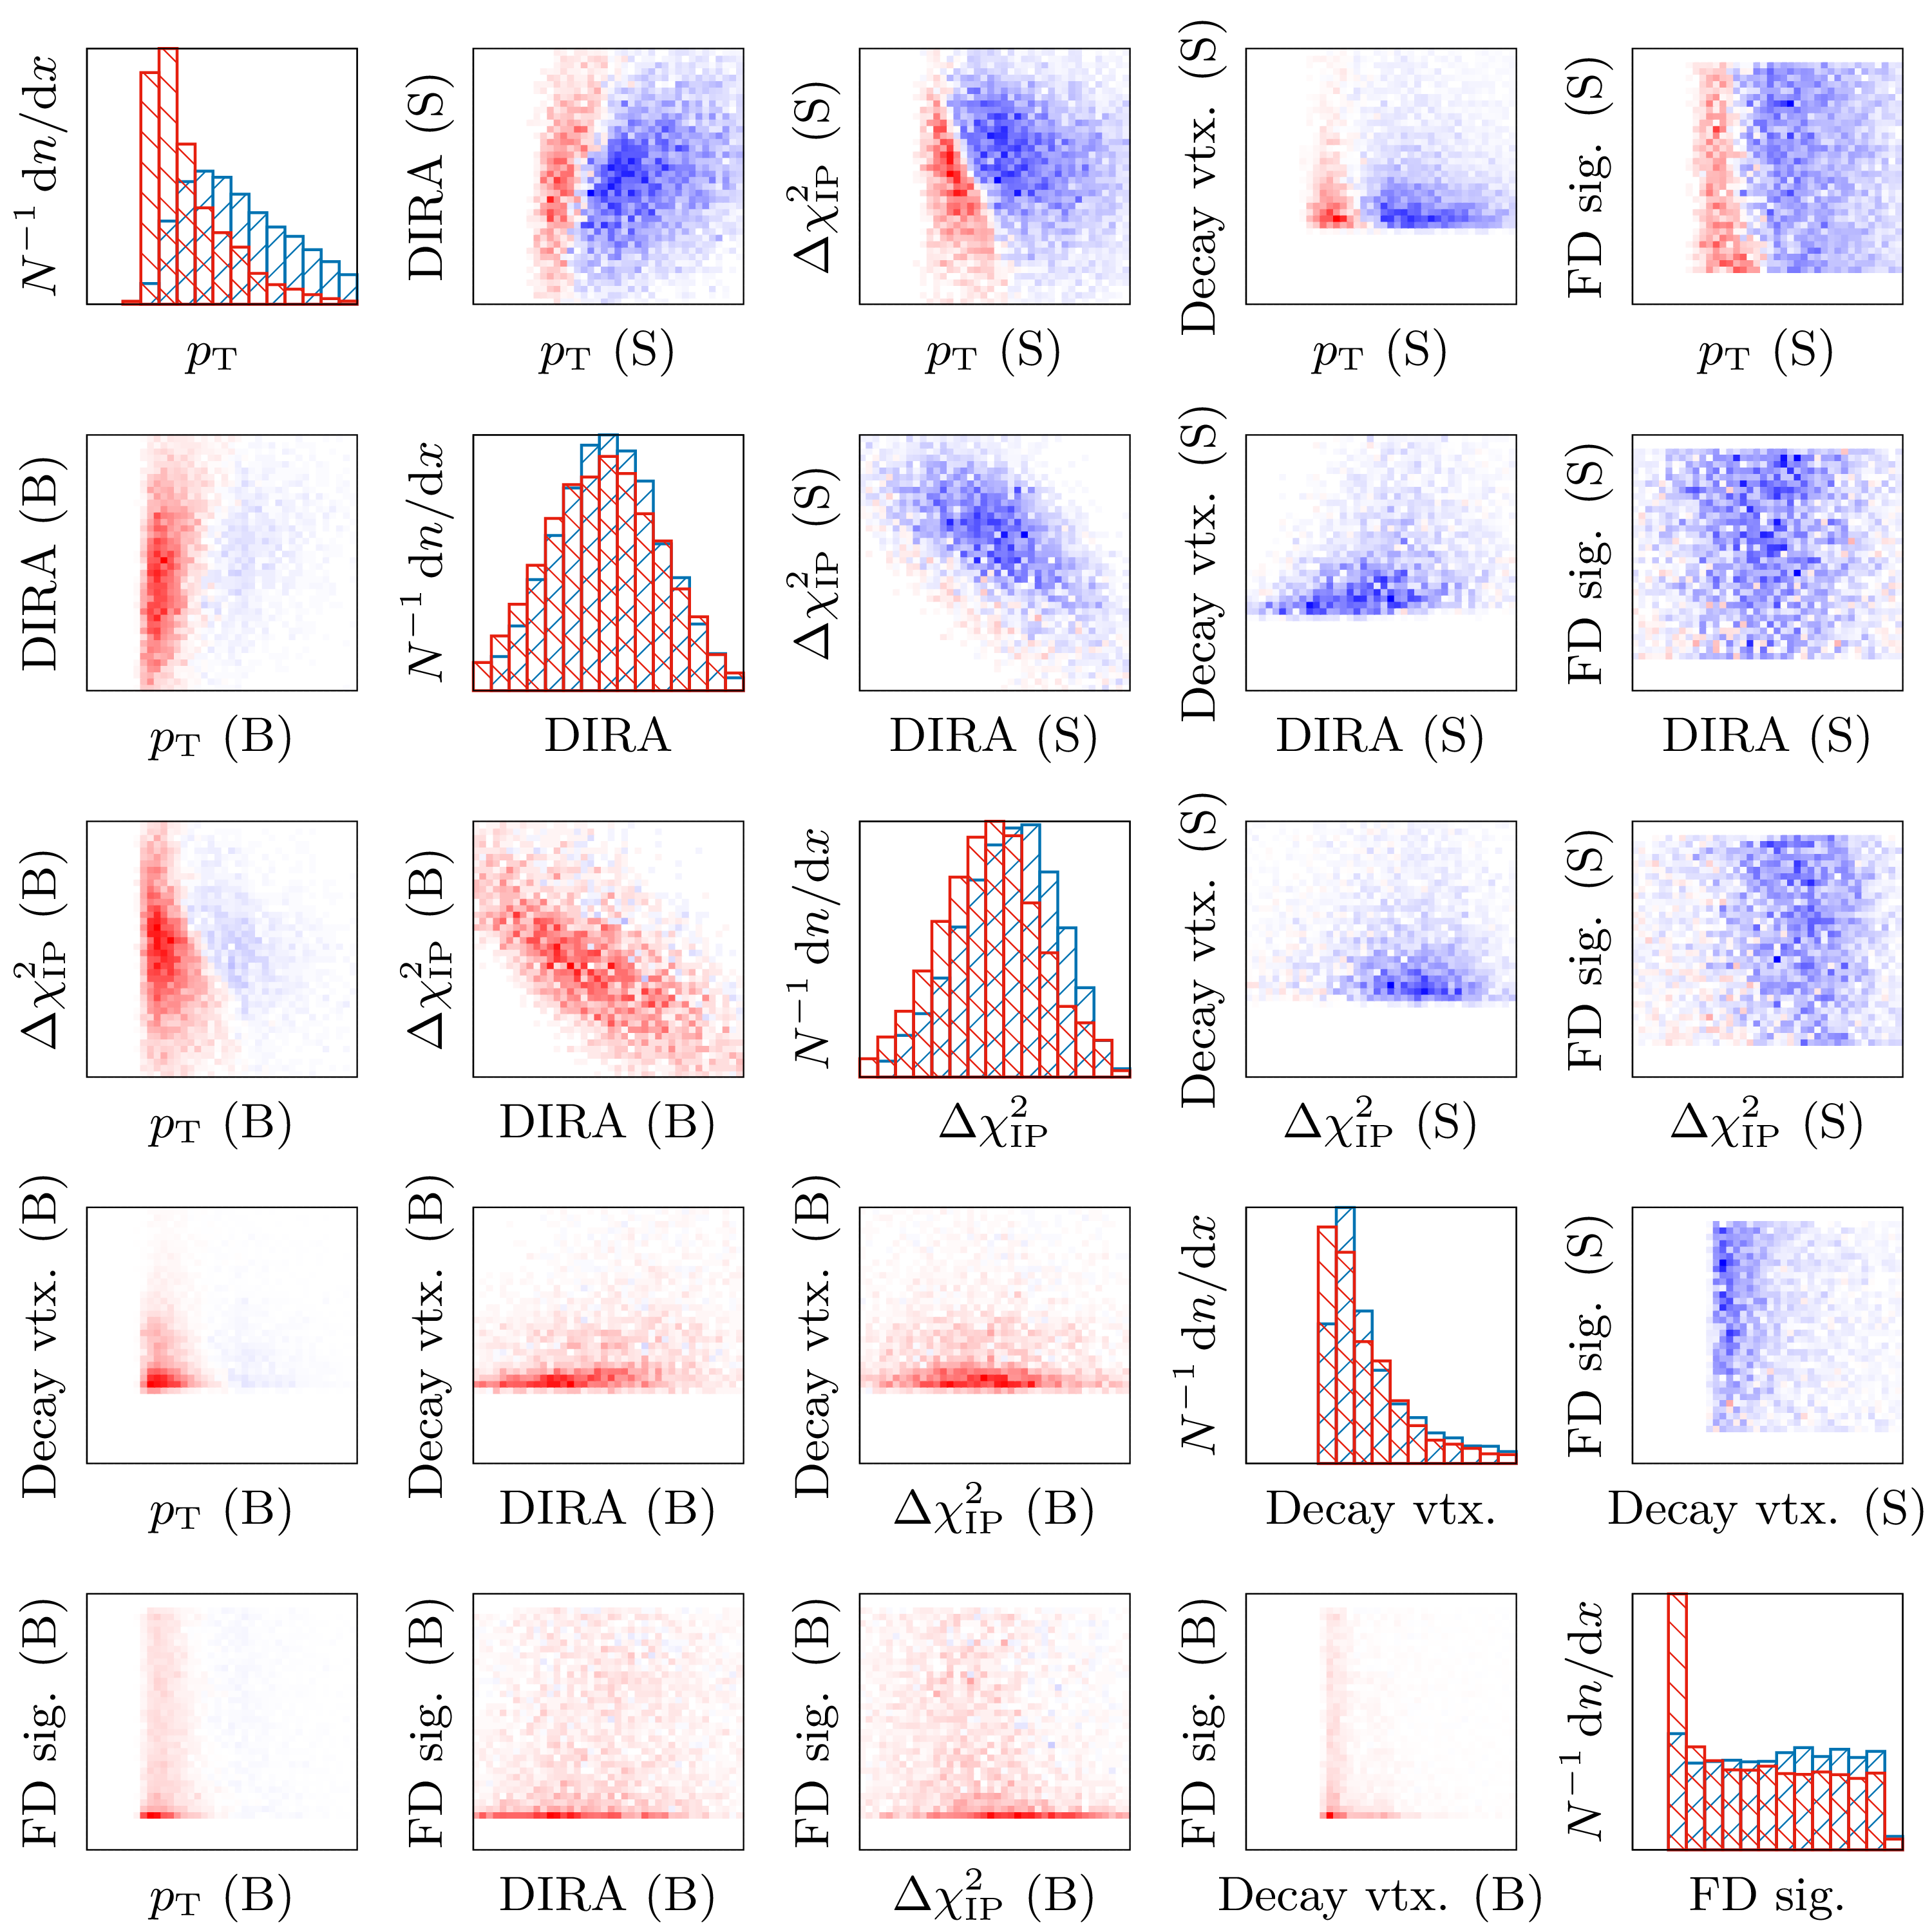
\includegraphics[height=.9\textheight]{mvaLz/mvaLz_corr_DD}\\
            (track type \textbf{DD})
        \end{column}
    \end{columns}
\end{frame}

\begin{frame}{Example: \Lz classifier}
    \begin{columns}
        \begin{column}{.45\textwidth}
            \scalebox{1.2}{\Lz classifier}
            \begin{itemize}
                \item 5 features of $\{ \Lz \}$
                \item Separate classifiers for LL and \textbf{DD}
                \item Optimize hyper-parameters of \textcolor{vertexDarkRed}{5 classifiers} using grid search w.r.t.\ ROC-AUC\ftnt{} value
            \end{itemize}
        \end{column}
        \begin{column}{.5\textwidth}
            \centering
            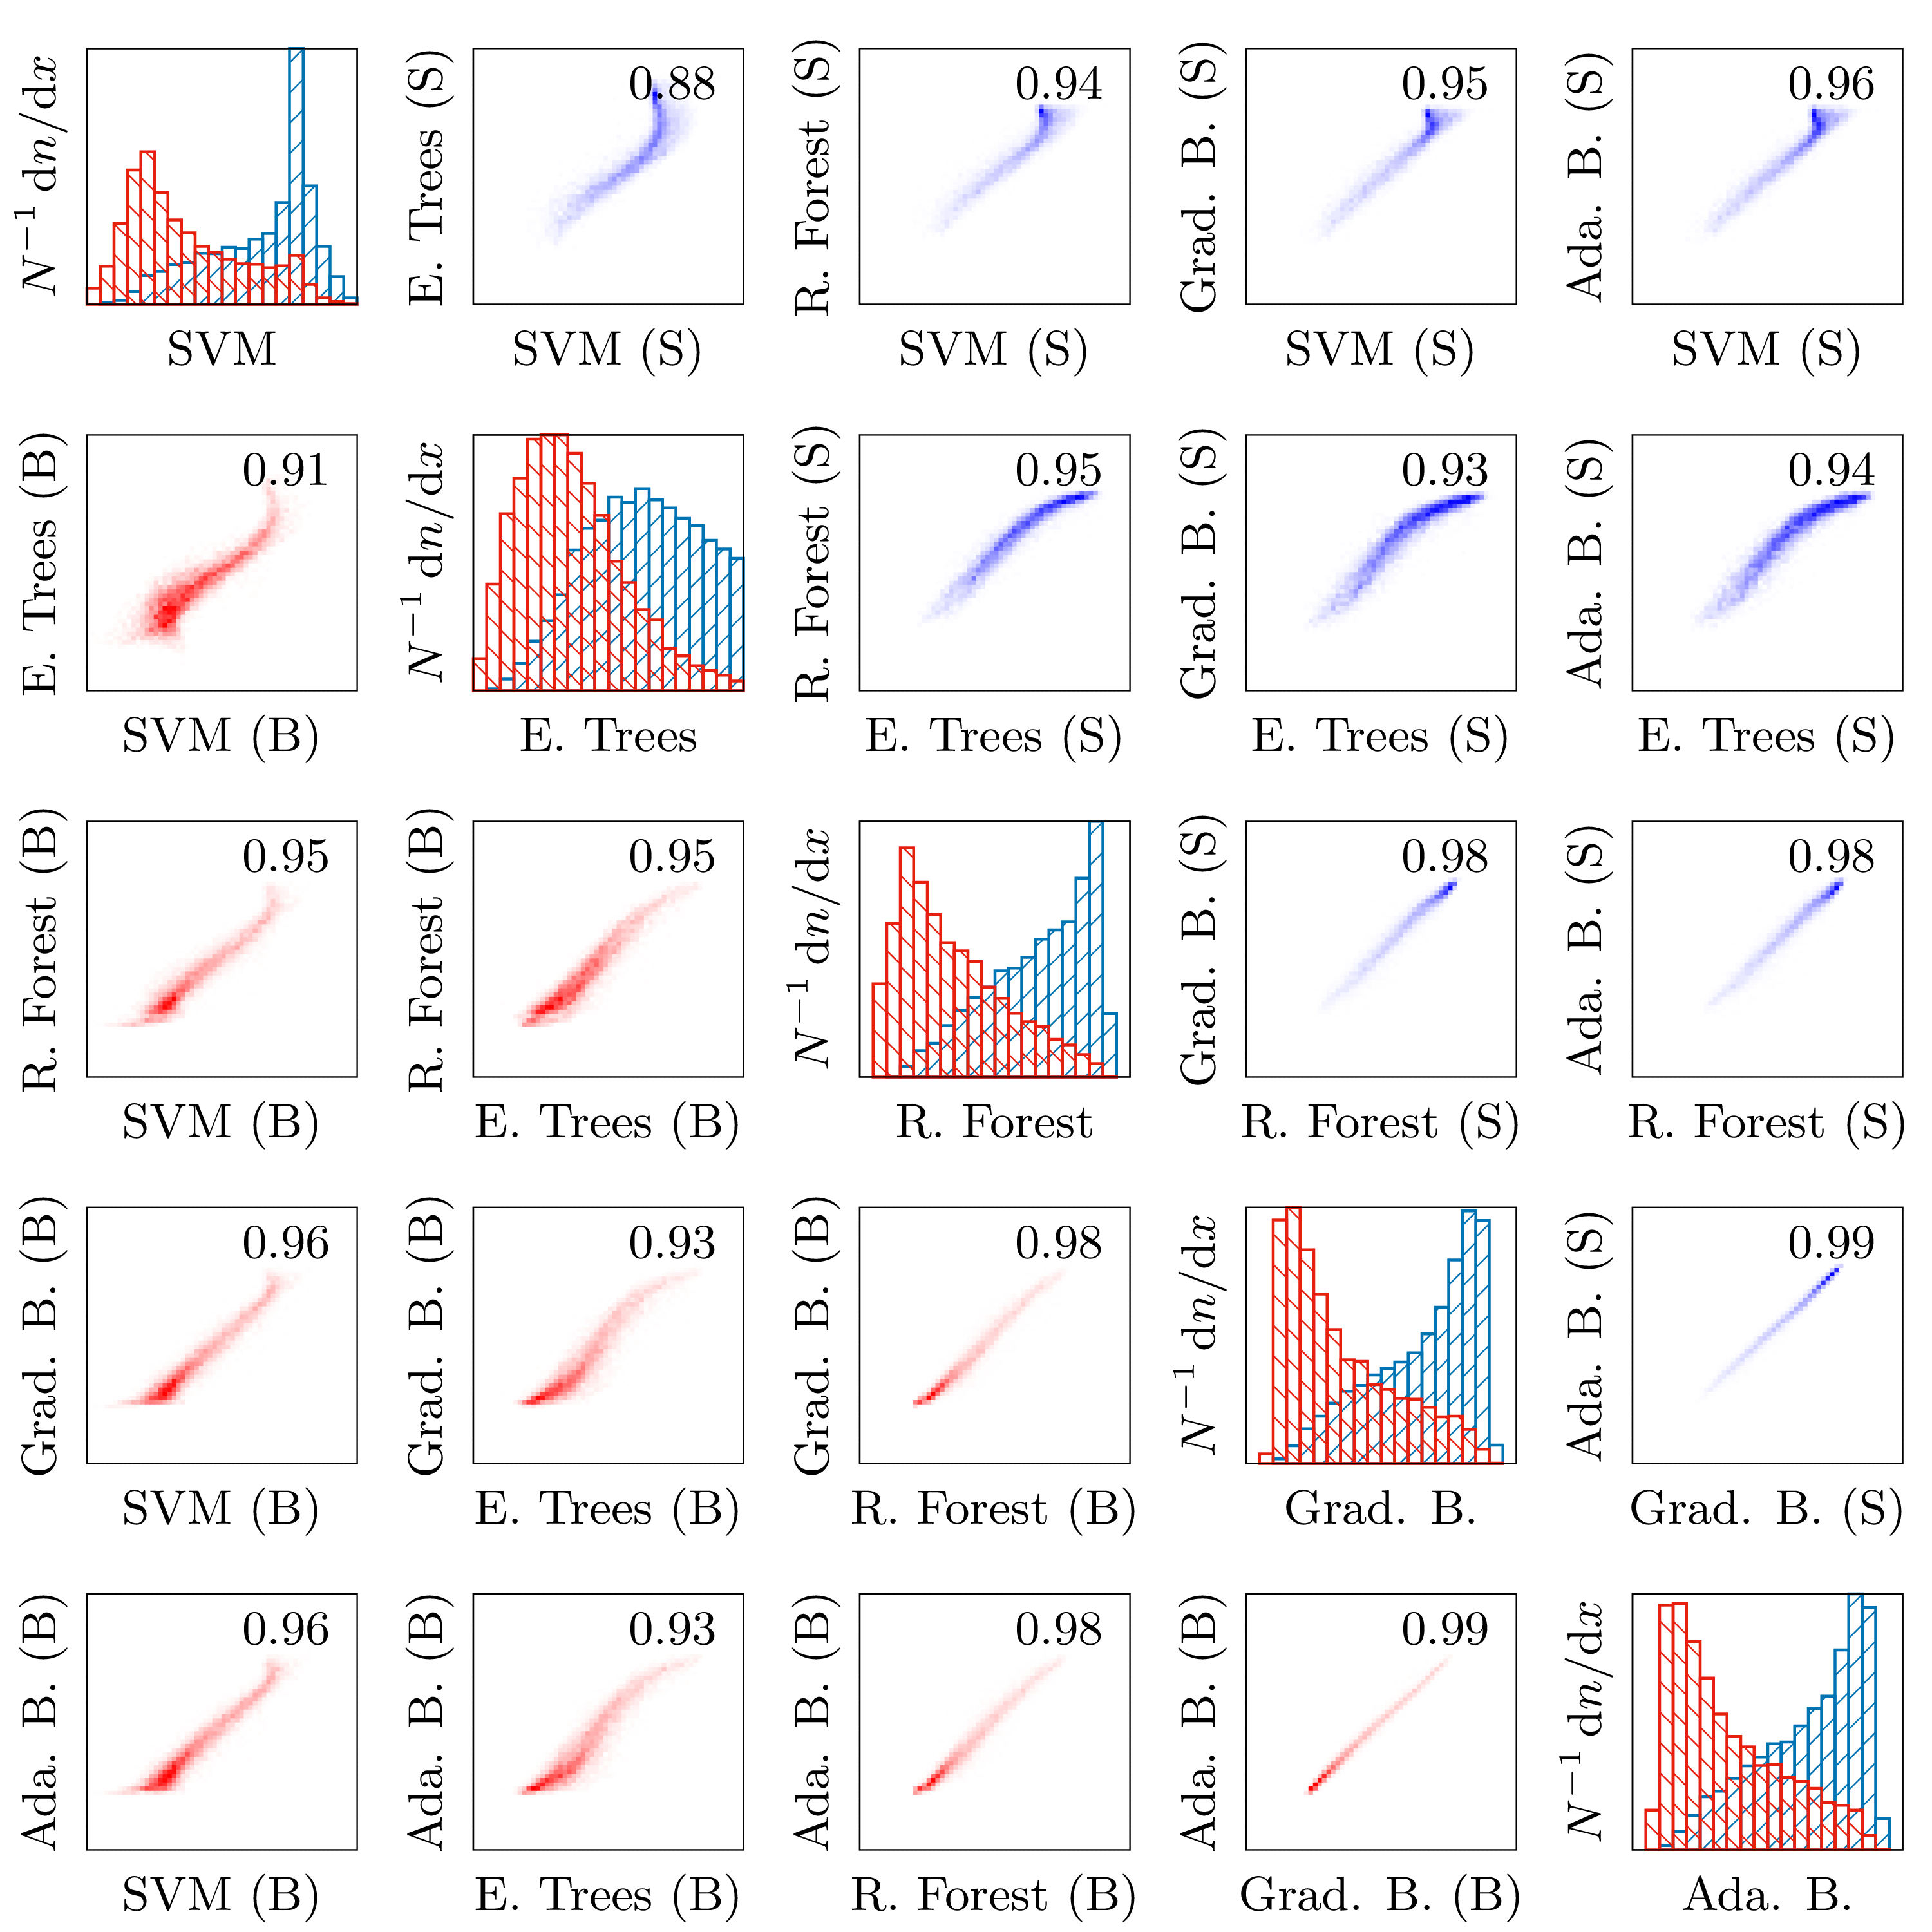
\includegraphics[height=.9\textheight]{mvaLz/stack_features_DD}\\
            (track type \textbf{DD})
        \end{column}
    \end{columns}
\end{frame}

\begin{frame}{Example: \Lz classifier}
    \begin{columns}
        \begin{column}{.45\textwidth}
            \scalebox{1.2}{\Lz classifier}
            \begin{itemize}
                \item 5 features of $\{ \Lz \}$
                \item Separate classifiers for LL and \textbf{DD}
                \item Optimize hyper-parameters of \textcolor{vertexDarkRed}{5 classifiers} using grid search w.r.t.\ ROC-AUC\ftnt{} value
            \end{itemize}
        \end{column}
        \begin{column}{.5\textwidth}
            \centering
            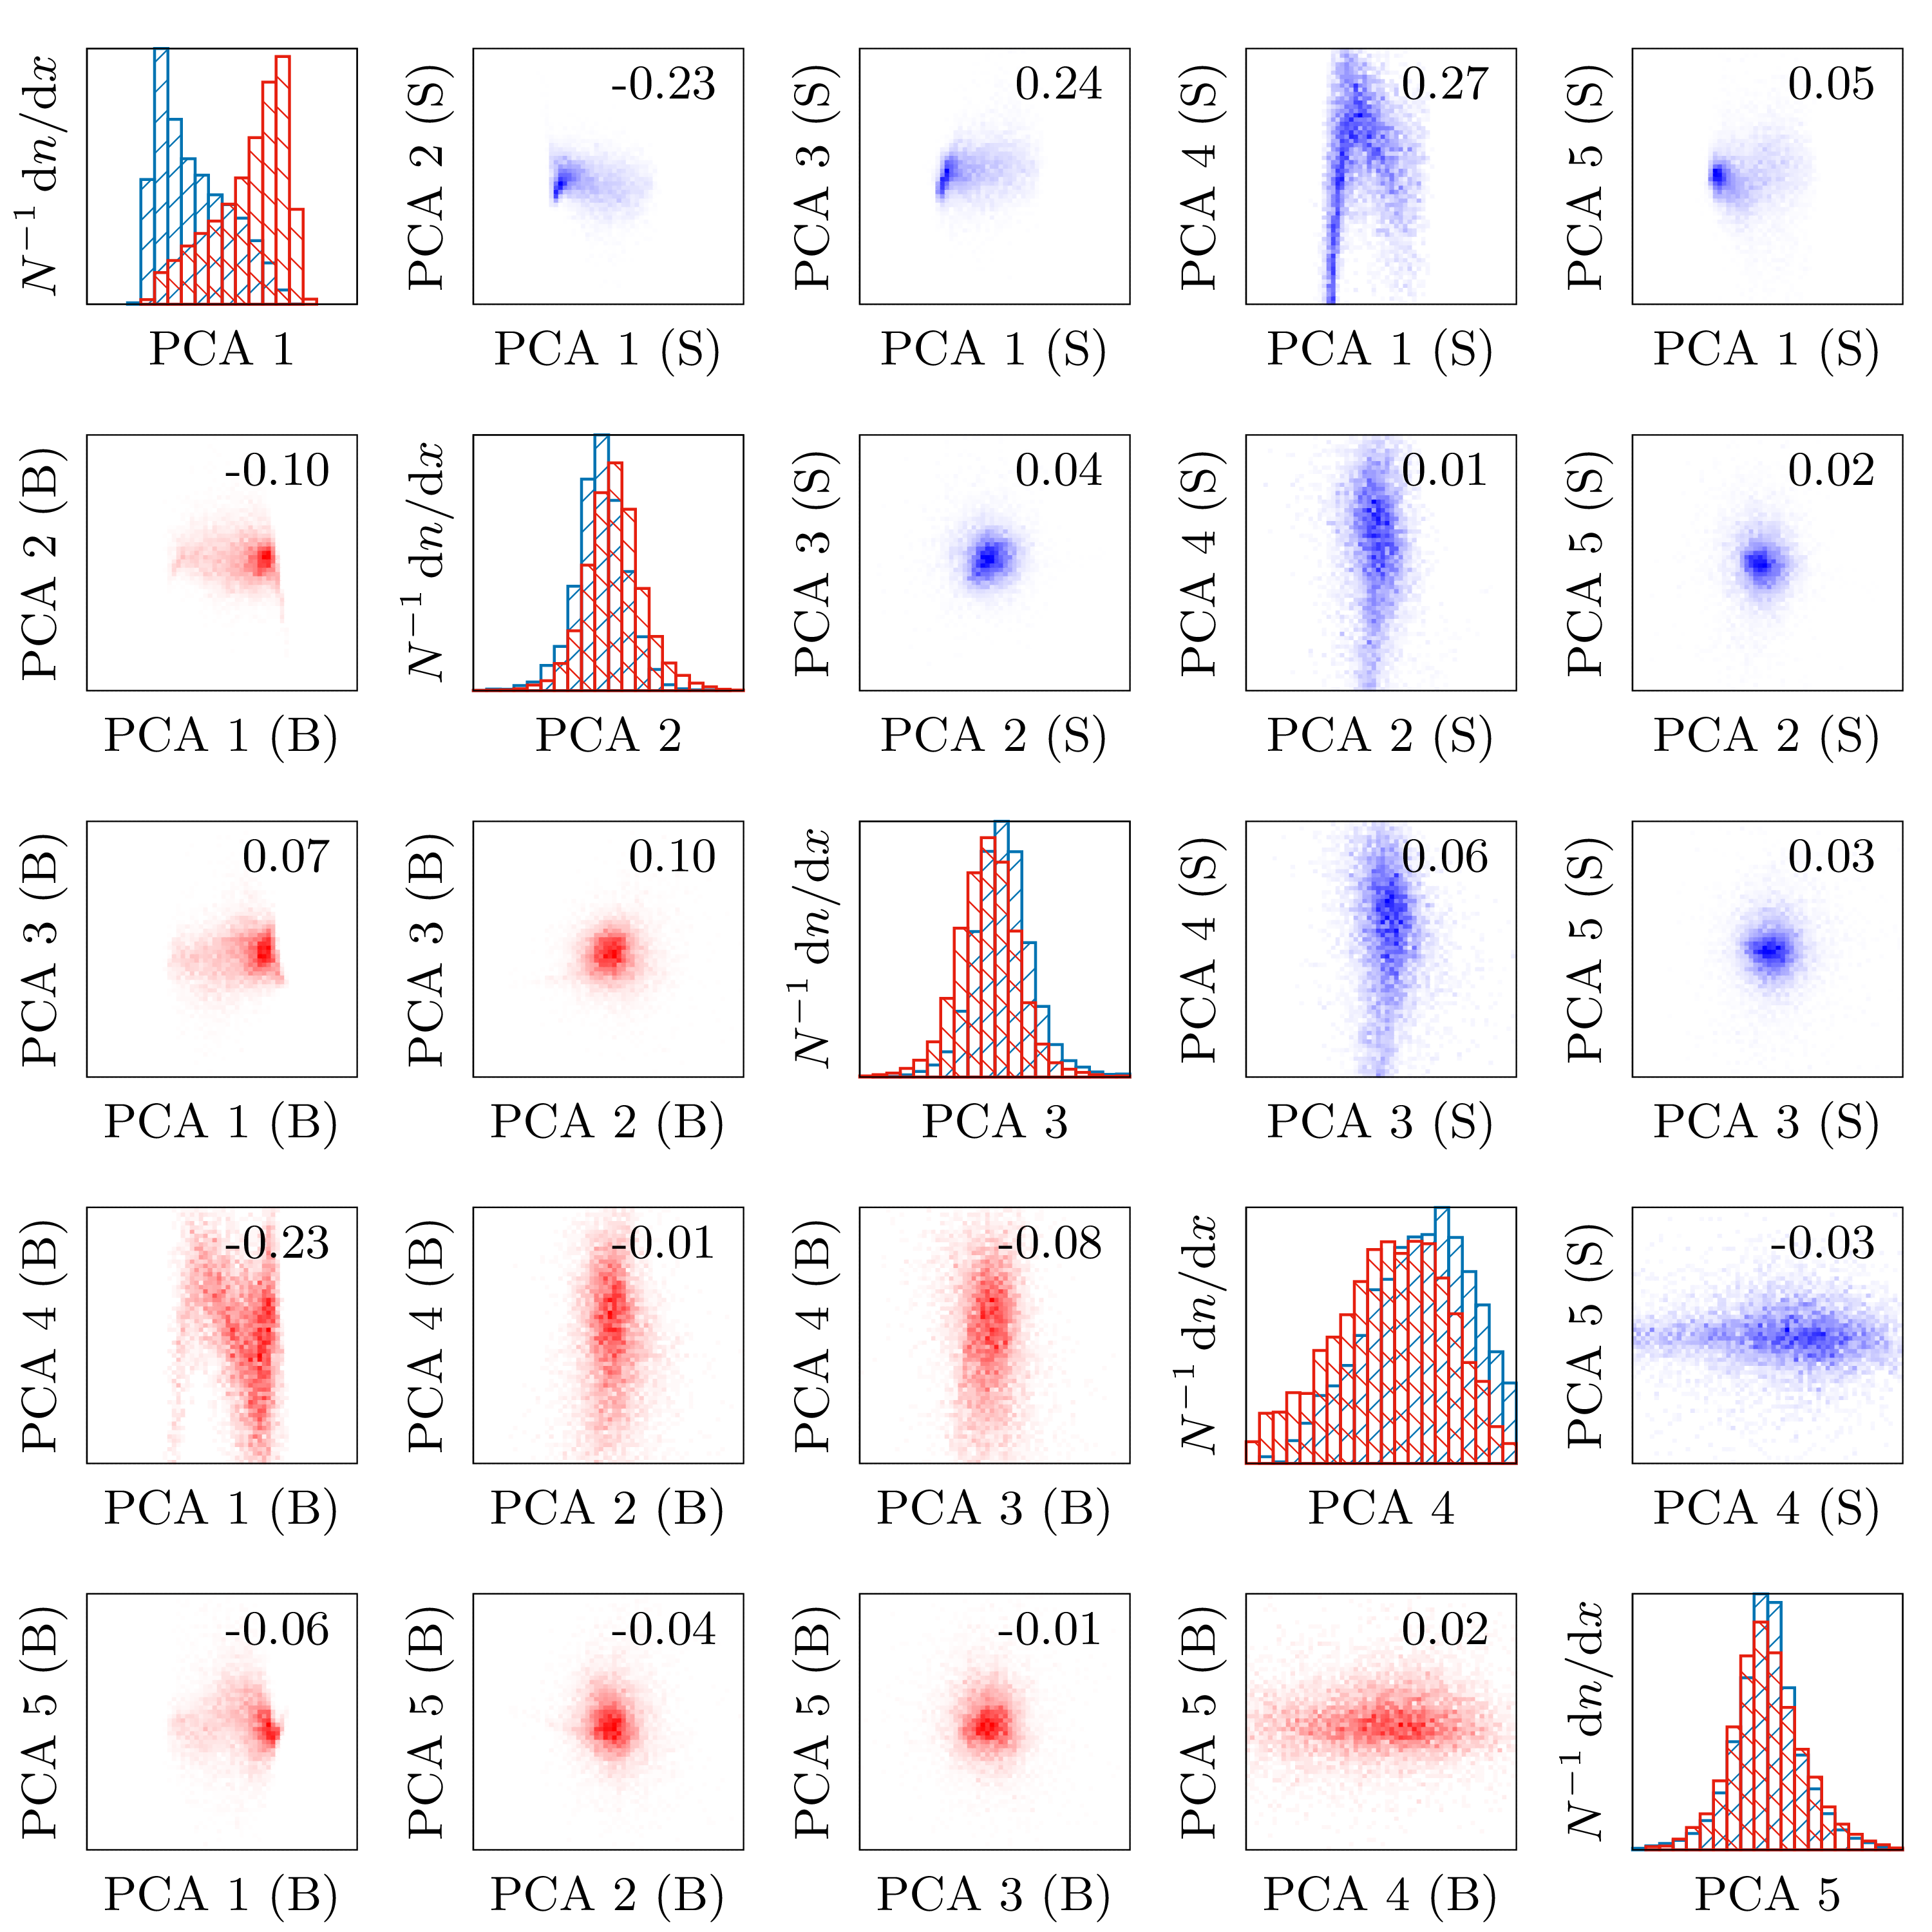
\includegraphics[height=.9\textheight]{mvaLz/stack_pcafeatures_DD}\\
            (track type \textbf{DD})
        \end{column}
    \end{columns}
\end{frame}

\begin{frame}{Fusion of high level classifiers}
    \begin{columns}
        \begin{column}{.5\textwidth}
            \centering
            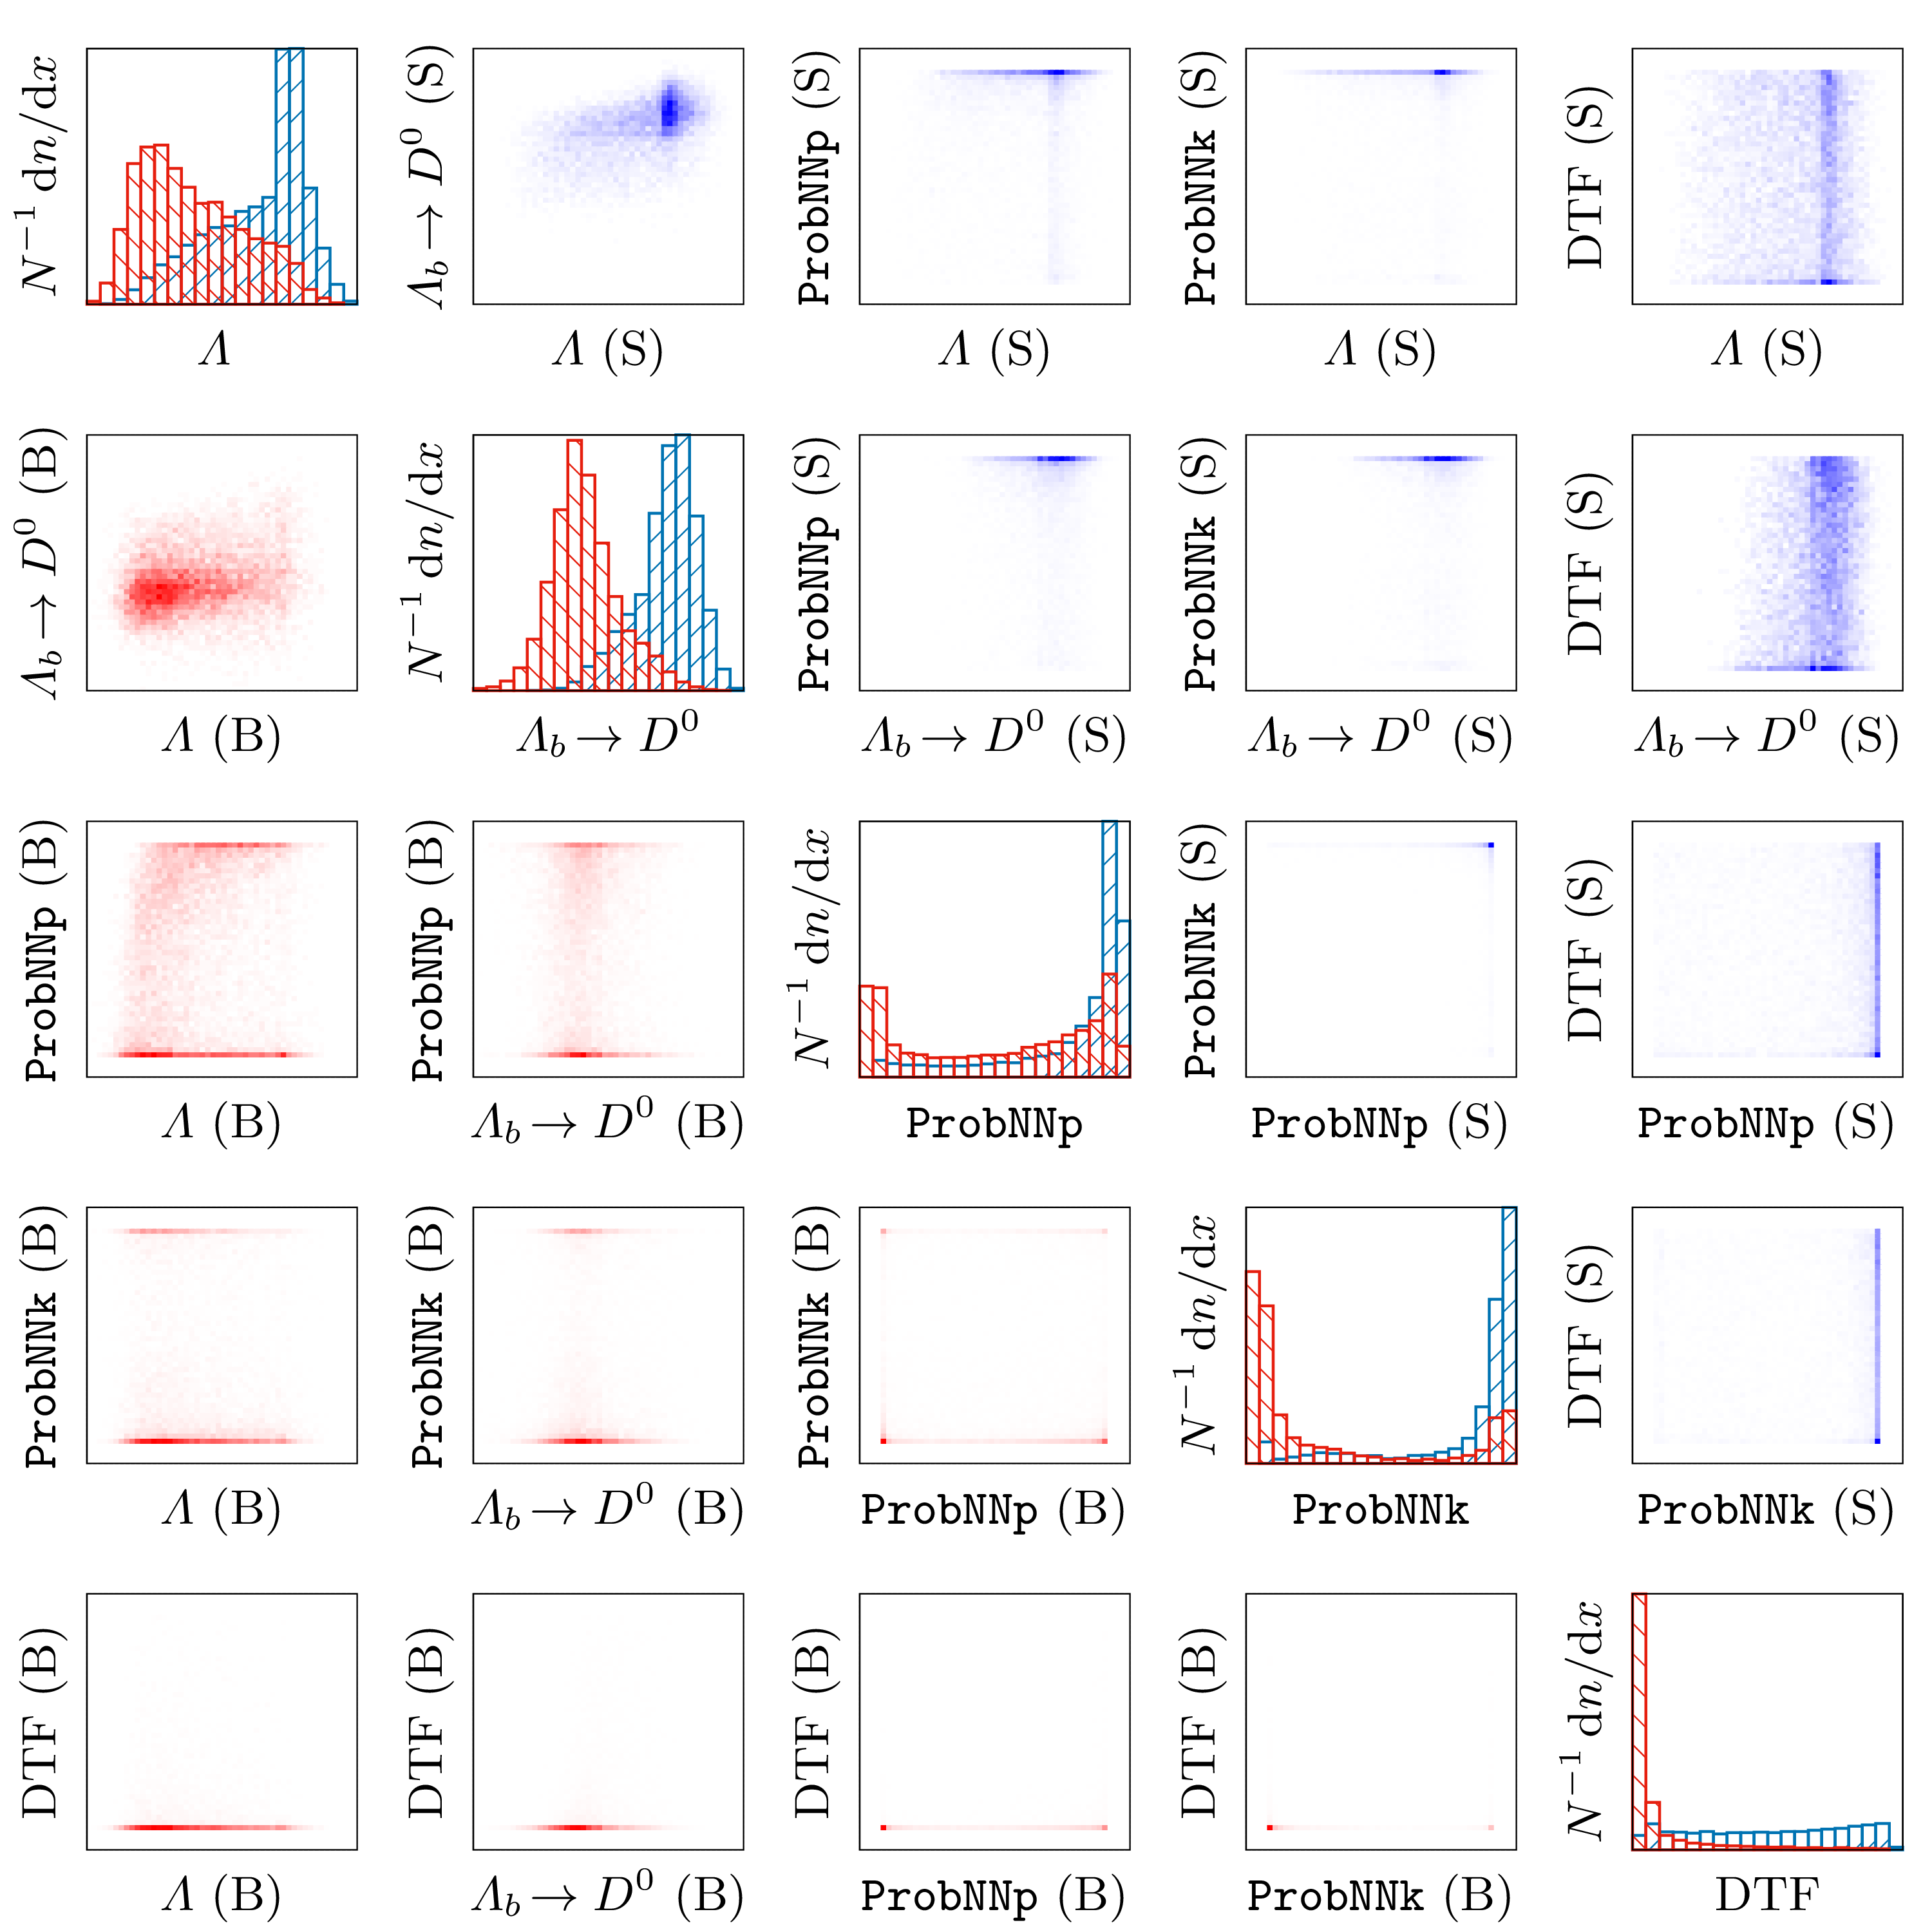
\includegraphics[height=.9\textheight]{mva/features_DD}\\
            (track type DD)
        \end{column}
        \begin{column}{.45\textwidth}
            \scalebox{1.2}{Fusion of high level classifiers}
            \begin{itemize}
                \item Optimize rectangular cut classifier (to avoid MC fidelity issues\ftntdagger)
                \item \ldots using classifier outputs as features
                \begin{enumerate}
                    \item \Lz classifier
                    \item \Lb-\Dz classifier
                    \item \texttt{ProbNNp}
                    \item \texttt{ProbNNk}
                    \item Decay tree fit
                \end{enumerate}
                \item (Compare rect.\ cut clf.\ eff.\ against decision tree\ftntdagger)
            \end{itemize}
        \end{column}
    \end{columns}
\end{frame}

\begin{frame}{Classifier fusion}
    \begin{columns}
        \begin{column}{.5\textwidth}
            \scalebox{1.2}{Optimize rect.\ cut clf.}
            \begin{itemize}
                \item Minimize FPR\ftnt{} at given TPR\ftnt\ftnt{}
                \item Numerically noisy: use simulated annealing for finding minimum 
                \item Set thresholds at TPR $\approx 50\,\%$ (LL) and TPR $\approx 30\,\%$ (DD)
                \item (Refine \textit{optimal} TPR with in a second, tight max.\ step only using $\Lz / \Lb$-$\Dz$ classifiers\ftntdagger)
            \end{itemize}
        \end{column}
        \begin{column}{.5\textwidth}
            \only<1>{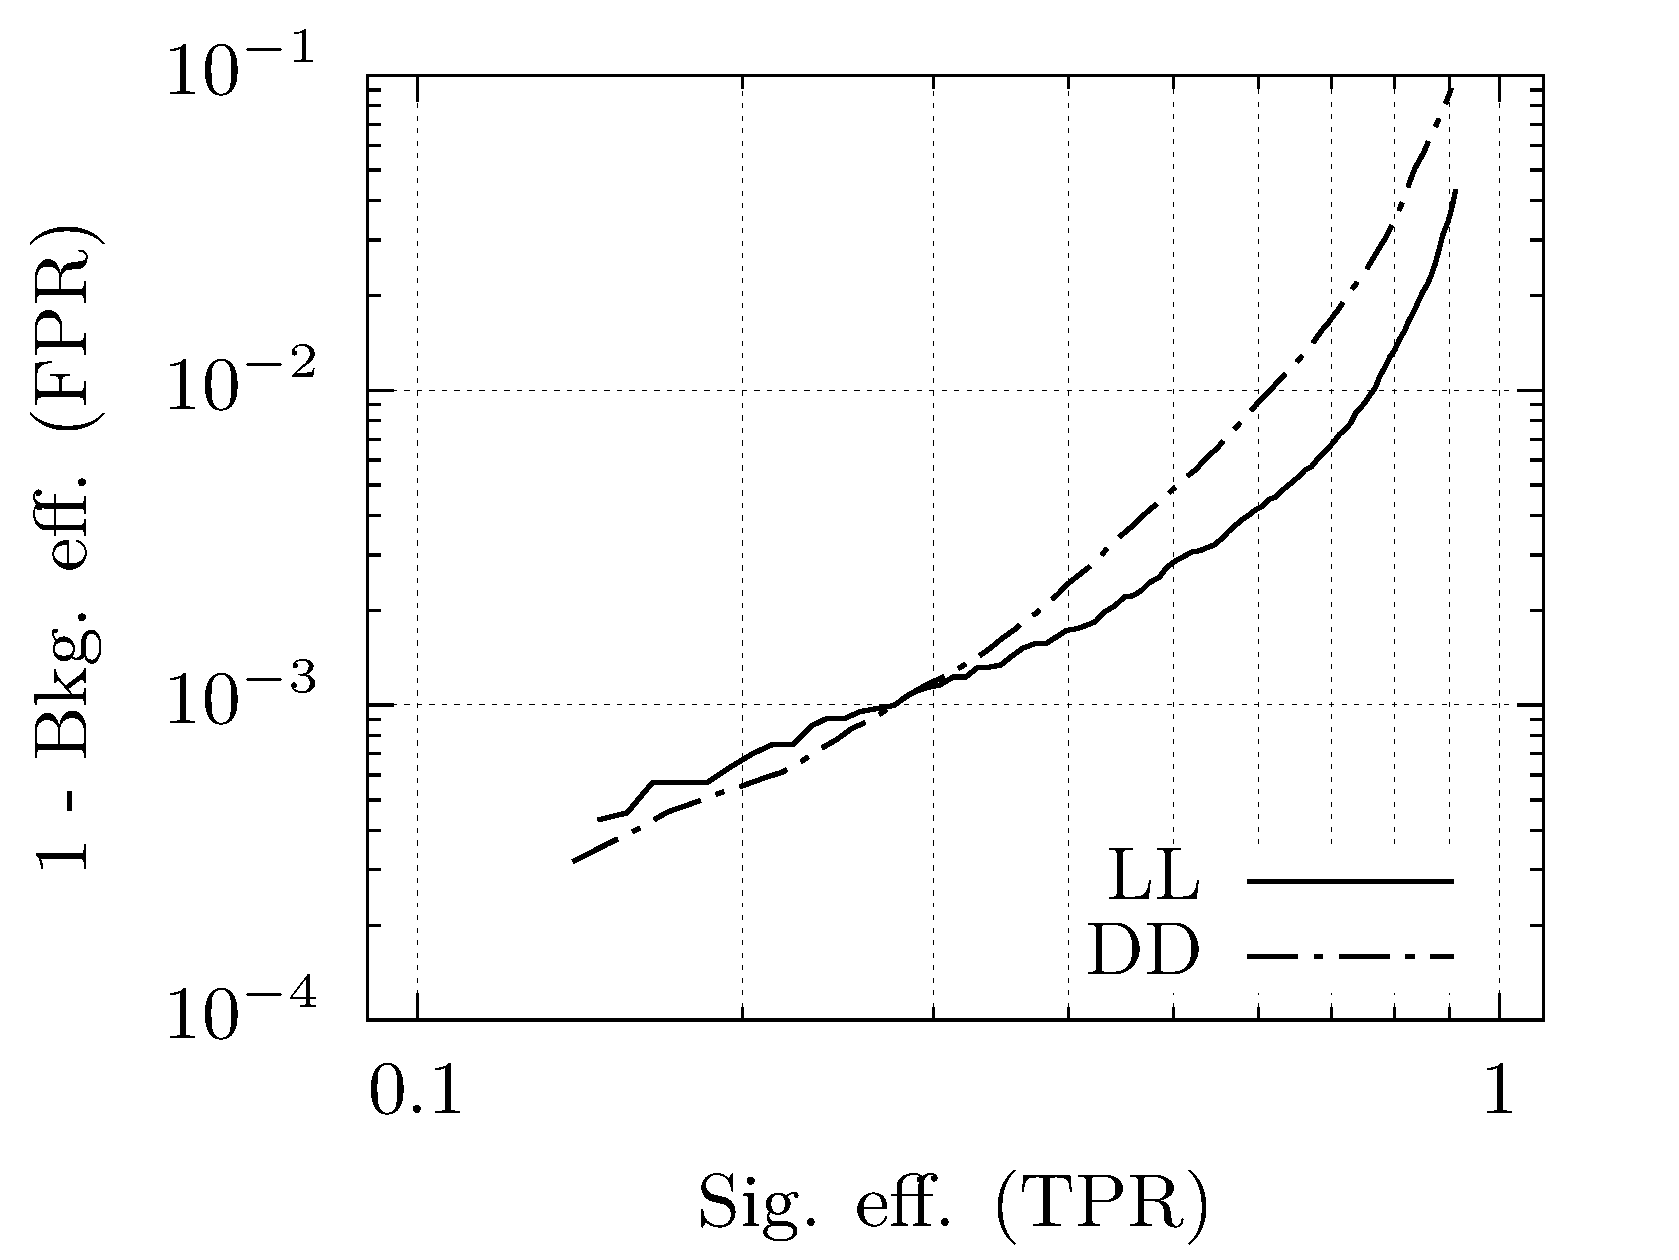
\includegraphics[scale=1.]{mva/roc}}%
            \only<2>{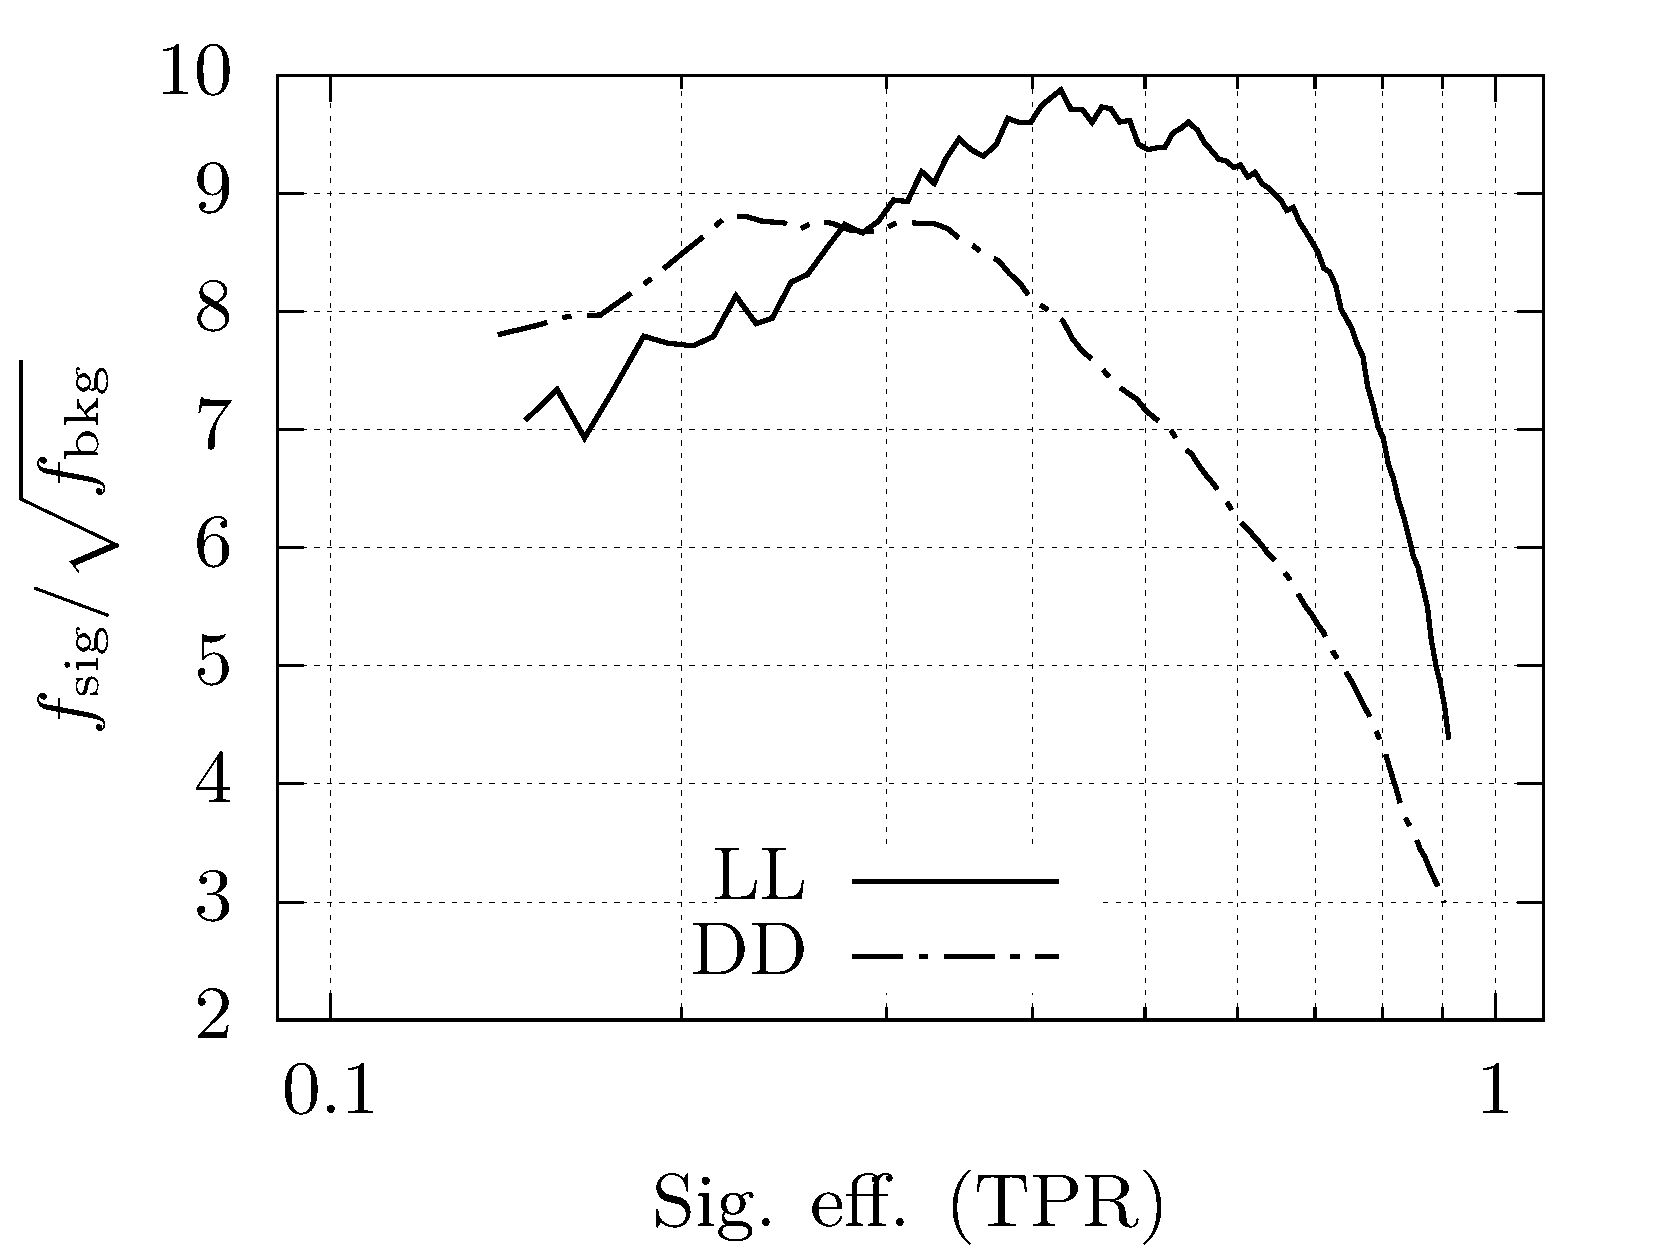
\includegraphics[scale=1.]{mva/significance}}%
        \end{column}
    \end{columns}

    \vspace{5mm}

    \footnotesize
    \phantom{\ftnt}\ftnt FPR: \underline{f}alse \underline{p}ositive \underline{r}ate, \ie{}, genuine bkg.\ predicted as sig.\\
    \ftnt\ftnt TPR: \underline{t}rue \underline{p}ositive \underline{r}ate, \ie{}, genuine sig.\ predicted as sig.
\end{frame}

\chapter{Yield Estimation}
\label{chap:fit}
\chapquote{With four parameters I can fit an elephant, and with five I can make him wiggle his trunk.}{Discovered by John von Neumann and exercised in Ref.~\cite{fourparams}.}
In this chapter we establish a fit model to extract signal yields from \num{260} signal candidates which are left after applying the previously outlined selection criteria to the \gls{runtwo} data sample.
This sparse data sample forces us to assume certain constraints and work with approximations.
We outline our assumptions and meticulously evaluate our fit model which eventually allows us to obtain signal yields and yield significances for the decay modes \decay{\Lb}{\Dz\Lz} and \decay{\Xibz}{\Dz\Lz}.

\section{The Fit Model}
\label{sec:fit_model}
Due to the small amount of available recorded signal candidates that passed the dedicated filtering steps and the absence of a precise background model in terms of statistics and polarization, we base our fit model onto the following assumptions:
\begin{itemize}
    \item The kinematic properties of the final states of signal and background events are following similar distributions, since they would have been filtered out by the preceding filtering steps otherwise. Their resolution is thus given by the signal shape of the \Lb or \Xibz baryon which are accessible through the respective \gls{mc} simulated decays in good approximation. This assumption is based on the short lifetime of the \bquark-hadrons w.r.t.\ the detector resolution, corresponding to a natural width of roughly $0.4\,\millievcc$.
    \item Due to the absence of a priori knowledge concerning the polarization of the \Dstarz and \Sz states in \decay{\Lb}{\Dstarz\Lz} and \decay{\Lb}{\Dz\Sz}, it is not possible to unfold the contribution of the latter from the broad $\Dz\piz$ and $\Dz\Pgamma$ decay modes of the former (\cf{}~Tab.~\ref{tab:apdx_partbkg_boundaries}). We verify this assumption with pseudo-experiments. The same assumption holds for the very broad (potential) background of \decay{\Xibz}{\Dz\Xiz} decays.
    \item For similar reasons we fix the yield ratio of the fit components of \decay{\Dstarz}{\Dz\piz} and \decay{\Dstarz}{\Dz\Pgamma} to its central value of $1.83$ measured by the \gls{babar} and \gls{besiii} collaborations and fitted by the \gls{pdg}~\cite{DstarBrs1,DstarBrs2,pdg}. Further, neither the ratio of the fitted yields of \decay{\Lb}{\Dz\Lz} and \decay{\Lb}{\Dstarz\Lz}, nor of \decay{\Xibz}{\Dz\Lz} and \decay{\Xibz}{\Dstarz\Lz}, nor of \decay{\Lb}{\Dz\Lz} and \decay{\Xibz}{\Dz\Lz} itself, should depend on the track type of the daughters of the \Lz baryon and are therefore fitted simultaneously for both track types. For \decay{\Lb}{\Dz\Lz} and \decay{\Xibz}{\Dz\Lz}, we cross-check this assumption with \gls{mc} simulated events. The double ratio (\cf{}~Tab.~\ref{tab:fit_ndatasamples}) is $1.026(23)$ and barely significantly deviates from one. The central value is less than $3\,\%$ which is negligible w.r.t.\ the total systematic uncertainties.
    \item The combinatorial background follows an exponential function which we parametrize according to Eq.~\eqref{eq:apdx_pdfs_exprel}. Our choice of parameter $k$'s sign is physically motivated but not required during the fits. We note that this implicitly includes the linear model $1 \pm kx$ for small values of $k$ and in particular the uniformly distributed (combinatorial) background for $k=0$.
\end{itemize}
The fit is applied to the combined invariant mass of \Dz and \Lz candidates and evaluated simultaneously on the unbinned datasets of simulated and recorded events of both track types.
The total amount of available events for each of these six samples is listed in Tab.~\ref{tab:fit_ndatasamples}.
\begin{table}[htbp]
    \centering
    \caption{Amount of \gls{mc} simulated and recorded events available for fitting. The fit is evaluated simultaneously in all six samples. Further, we give the (weighted) fraction for the \gls{mc} simulated events w.r.t.\ the amount of events $N$, after the preselection. The double ratio of these fractions is $1.025(24)$ and thus barely deviate from one significantly.}
    \label{tab:fit_ndatasamples}
    \begin{tabular}{l%
                    S[table-format=5.2]%
                    S[separate-uncertainty=false,table-format=2.1(2)]%
                    S[table-format=5.2]%
                    S[separate-uncertainty=false,table-format=2.2(2)]}
        \toprule
        & \multicolumn{2}{c}{{\Gls{LL}}} & \multicolumn{2}{c}{{\Gls{DD}}} \\
        & {$n$} & {$n/N$ [\%]} & {$n$} & {$n/N$ [\%]} \\
        \midrule
        %MC sim.\ \decay{\Lb}{\Dz\Lz} & 5682 & 36.0 \pm .4 & 5548 & 15.42 \pm .19 \\
        %MC sim.\ \decay{\Xibz}{\Dz\Lz} & 6244 & 35.0 \pm .4 & 6432 & 15.37 \pm .18 \\
        \gls{mc} sim.\ \decay{\Lb}{\Dz\Lz} & 5682 & 36.0 \pm .4 & 5548 & 13.81 \pm .19 \\
        \gls{mc} sim.\ \decay{\Xibz}{\Dz\Lz} & 6244 & 35.0 \pm .4 & 6432 & 13.27 \pm .18 \\
        rec.\ data & 113 & {--} & 147 & {--} \\
        \bottomrule
    \end{tabular}
\end{table}
The fit model is a normalized, weighted sum of the three components $\mathcal{S}$, $\mathcal{D}$ and $\mathcal{B}$, describing the \Lb / \Xibz signal, the \Dstarz background and the combinatorial background, respectively,
\begin{equation}
    \label{eq:fit_likelihood}
    \mathcal{L} := \left\lVert \begin{pmatrix} \mathcal{S} \\ \mathcal{D} \\ \mathcal{B} \end{pmatrix} \right\rVert_{\vec f} \equiv (1-f_1) \times \mathcal{S} \, + \, (1-f_2)f_1 \times \mathcal{D} \, + \, f_1 f_2 \times \mathcal{B} \,.
\end{equation}
For brevity we introduced the shorthand notation 
\begin{equation*}
    \left\lVert \vec{\mathcal{V}} \right\rVert_{\vec f} \, := \sum_{j=1}^n p_j \! \left( \vec{f}\, \right) \times \mathcal{V}_j \,,
\end{equation*}
which wraps the (normalized) weighted sum of the components $\vec{\mathcal{V}} = (\mathcal{V}_1, \ldots \mathcal{V}_n)$ with weights $\vec{f} = (f_1, \ldots f_{n-1})$, by defining $p_j$ according to
\begin{align*}
    p_j &:= (1-f_j) \prod_{i=1}^{j-1} f_i \quad \text{for } j < n \,, \\
    p_n &:= \prod_{i=1}^{n-1} f_i \,.
\end{align*}
Using this notation we define $\mathcal{S}$ and $\mathcal{D}$ for \Lb and \Xib:
\begin{align*}
    \mathcal{S} &:= \left\lVert \begin{pmatrix} \mathcal{G}^{(2)}(\Xib) \\ \mathcal{G}^{(2)}(\Lb) \end{pmatrix} \right\rVert_{f_s} \,, \\
    \mathcal{D} &:= \left\lVert \begin{pmatrix} \mathcal{K}(\Xib) * \mathcal{G}^{(2)}_c(\Lb) \\ \mathcal{K}(\Lb) * \mathcal{G}^{(2)}_c(\Lb) \end{pmatrix} \right\rVert_{f_\Dstar} \,,
\end{align*}
where $\mathcal{G}^{(2)}$ ($\mathcal{G}_c^{(2)}$) refers to a double Gaussian with shared (zero) mean
\begin{equation*}
    \mathcal{G}^{(2)} := \left\lVert \begin{pmatrix} \mathcal{G}_1 \\ \mathcal{G}_2 \end{pmatrix} \right\rVert_{f_\mathcal{G}} \,,
\end{equation*}
and $\mathcal{K}$ are the kernel functions for \decay{\Lb/\Xibz}{\Dstarz\Lz} decays as introduced in Appx.~\ref{chap:apdx_partbkg}.
More precisely, the latter is composed of the fixed superposition of the \Dstarz modes \decay{\Dstarz}{\Dz\piz} and \decay{\Dstarz}{\Dz\Pgamma}, and is convoluted with the resolution function as motivated previously.
During evaluation of the likelihood for the \gls{mc} simulated samples, the corresponding signal component is separated by enforcing $(f_1,f_s)=(0,0)$ or $(f_1,f_s)=(0,1)$.
Besides that, $f_2$ and $f_s$ are constrained to not depend on the track type, whereas $f_1$ is allowed to vary among different track types.
Similarly, the Gaussian shapes
\begin{align*}
    \mathcal{G}_1 &:= \begin{cases}
        \mathcal{G}(x|\mu,\sigma_1^\text{(LL)}) & \text{for \gls{LL}} \,,\\
        \mathcal{G}(x|\mu + \Delta \mu,\sigma_1^\text{(DD)}) & \text{for \gls{DD}} \,,\\
    \end{cases} \\ 
    \mathcal{G}_2 &:= \begin{cases}
        \mathcal{G}(x|\mu,\sigma_2^\text{(LL)}) & \text{for \gls{LL}} \,,\\
        \mathcal{G}(x|\mu + \Delta \mu,\sigma_2^\text{(DD)}) & \text{for \gls{DD}} \,,\\
    \end{cases}
\end{align*}
are allowed to deviate among different track types.
This includes $f_\mathcal{G}$ and the shared mean value, technically encoded by the shared shift $\Delta \mu$.

The unbinned, single entry fit w.r.t.\ Eq.~\eqref{eq:fit_likelihood} is performed with different configurations of fixed and floating parameters and within the two different mass ranges $5.5 \le m(\Dz\Lz) \le 6\,\gevcc$ and $5.2 \le m(\Dz\Lz) \le 6\,\gevcc$.
We tried different combinations of floating and fixed polarizations in the \Dstar kernel functions $\mathcal{K}$ but could not obtain reasonable results.
Thus we stick to an unpolarized description, leaving with six configurations which yield converging fits:
\begin{enumerate}
    \item Using the narrow mass range $5.5 \le m(\Dz\Lz) \le 6\,\gevcc$ cuts off most of the \decay{\Lb}{\Dstarz\Lz} background. The value of the fraction $f_\Dstar$ is thus fixed to zero, making $f_2$ the yield of \decay{\Xibz}{\Dstarz\Lz} and leaves 22 floating parameters that are optimized by the fit. The fit converges successfully, but prefers $f_2=1$ (upper boundary). The fitted values are listed in Tab.~\ref{tab:fit_fitres1}. In Fig.~\ref{fig:fit_hLbM_data_fit1} we show the accumulated projection of recorded data and the fit function. Other projections are shown in Appx.~\ref{chap:apdx_fitsupp}. 
    \item In order to extract the significance of the signal yields observed with the previous fit, we fix all contributions coming from \gls{mc} simulated events, keep $f_\Dstar$ fixed to zero and disable \Dstarz contributions in accordance with the previous results by enforcing $f_2$ to one. The likelihood Eq.~\eqref{eq:fit_likelihood} is then maximized with $f_s$ fixed to one and zero, corresponding to the removal of the \Xibz and \Lb component, respectively, and then compared with the results when $f_s$ is a floating parameter. The projection of recorded data of the former two fits is shown in Fig.~\ref{fig:fit_hLbM_data_fit23} together with respective fit projections. Since the fits with $f_s$ set to one and zero have exactly one \gls{dof} less than the fit which allows floating values for $f_s$, the difference of their respective log-likelihoods $\Delta \! \ln \mathcal{L}$ can be used to approximate the (statistical) significance $S = \sqrt{-2 \Delta \! \ln \mathcal{L}}$. Doing so, we estimate a signal significance of $S=5.5$ and $S=1.8$ for the decays \decay{\Lb}{\Dz\Lz} and \decay{\Xibz}{\Dz\Lz}, respectively. This approximation is based on Wilks theorem~\cite{wilkstheorem} whose applicability is tested with a pseudo-experiment in Sec.~\ref{sec:fit_wilkstest}.
    \item In order to estimate the significance of the \decay{\Lb}{\Dstarz\Lz} background, we reevaluate the fit using the broad mass range $5.2 \le m(\Dz\Lz) \le 6\,\gevcc$ and keep all fit parameters floating. The invariant mass distributions and fit projections of recorded data are shown in Fig.~\ref{fig:fit_hLbM_data_fit3}. We note that $f_2$ does not depend on the track type, presumably causing the combinatorial background for \gls{LL} tracks to overshoot at low $m(\Dz\Lz)$ values.
    \item Extending the fit model and allowing $f_2$ to take on different values for different tack types fixes the issues that we observed during the previous fit (\cf{}~Fig.~\ref{fig:fit_hLbM_data_fit4}). The fitted values for $f_2$ are $0.66(12)$ and $0.98(9)$ for \gls{LL} and \gls{DD} tracks, respectively, differ strongly and cannot be physically motivated.
    \item We repeat the fit in configuration 3 but this time replace the resolution function used for smearing the \Dstarz kernel functions $\mathcal{K}$ with the centralized \Xibz signal shape.
    \item We artificially enrich the data set by drawing $n$ instances from a smeared, unpolarized \decay{\Lb}{\Dz\Sz} distribution, as derived in Appx.~\ref{chap:apdx_partbkg}, to the recorded data sample. The amount of drawn instances $n$ is fixed to $\sfrac{1}{3}$ of the fitted \Lb signal yield in accordance with our estimations in Sec.~\ref{sec:isospin}. Since we expect genuine \decay{\Lb}{\Dz\Sz} in the recorded data, we consider this is a conservative approximation of this background. We abstain from a similar cross-check of \decay{\Xibz}{\Dz\Sz} decays due to the low \decay{\Xibz}{\Dz\Lz} yields and the unclear branching ratio of the \Sz mode.
    \item In the previous configurations the mass difference $m(\Xibz) - m(\Lb)$ was fixed to its nominal value $172.5\,\mevcc$. The \gls{pdg} states an uncertainty of $0.4\,\mevcc$ which we use to test the sensitivity of our model to this value by setting $m(\Xibz) - m(\Lb)$ to $172.1\,\mevcc$ (7a) and $172.9\,\mevcc$ (7b).
\end{enumerate}
Regarding the yields of the decays \decay{\Lb}{\Dz\Lz} and \decay{\Xibz}{\Dz\Lz}, the results of the outlined fits are compatible and give almost identical values for both modes as listed in Tab.~\ref{tab:fit_rawyields}.

\begin{figure}[htbp]
    \centering
    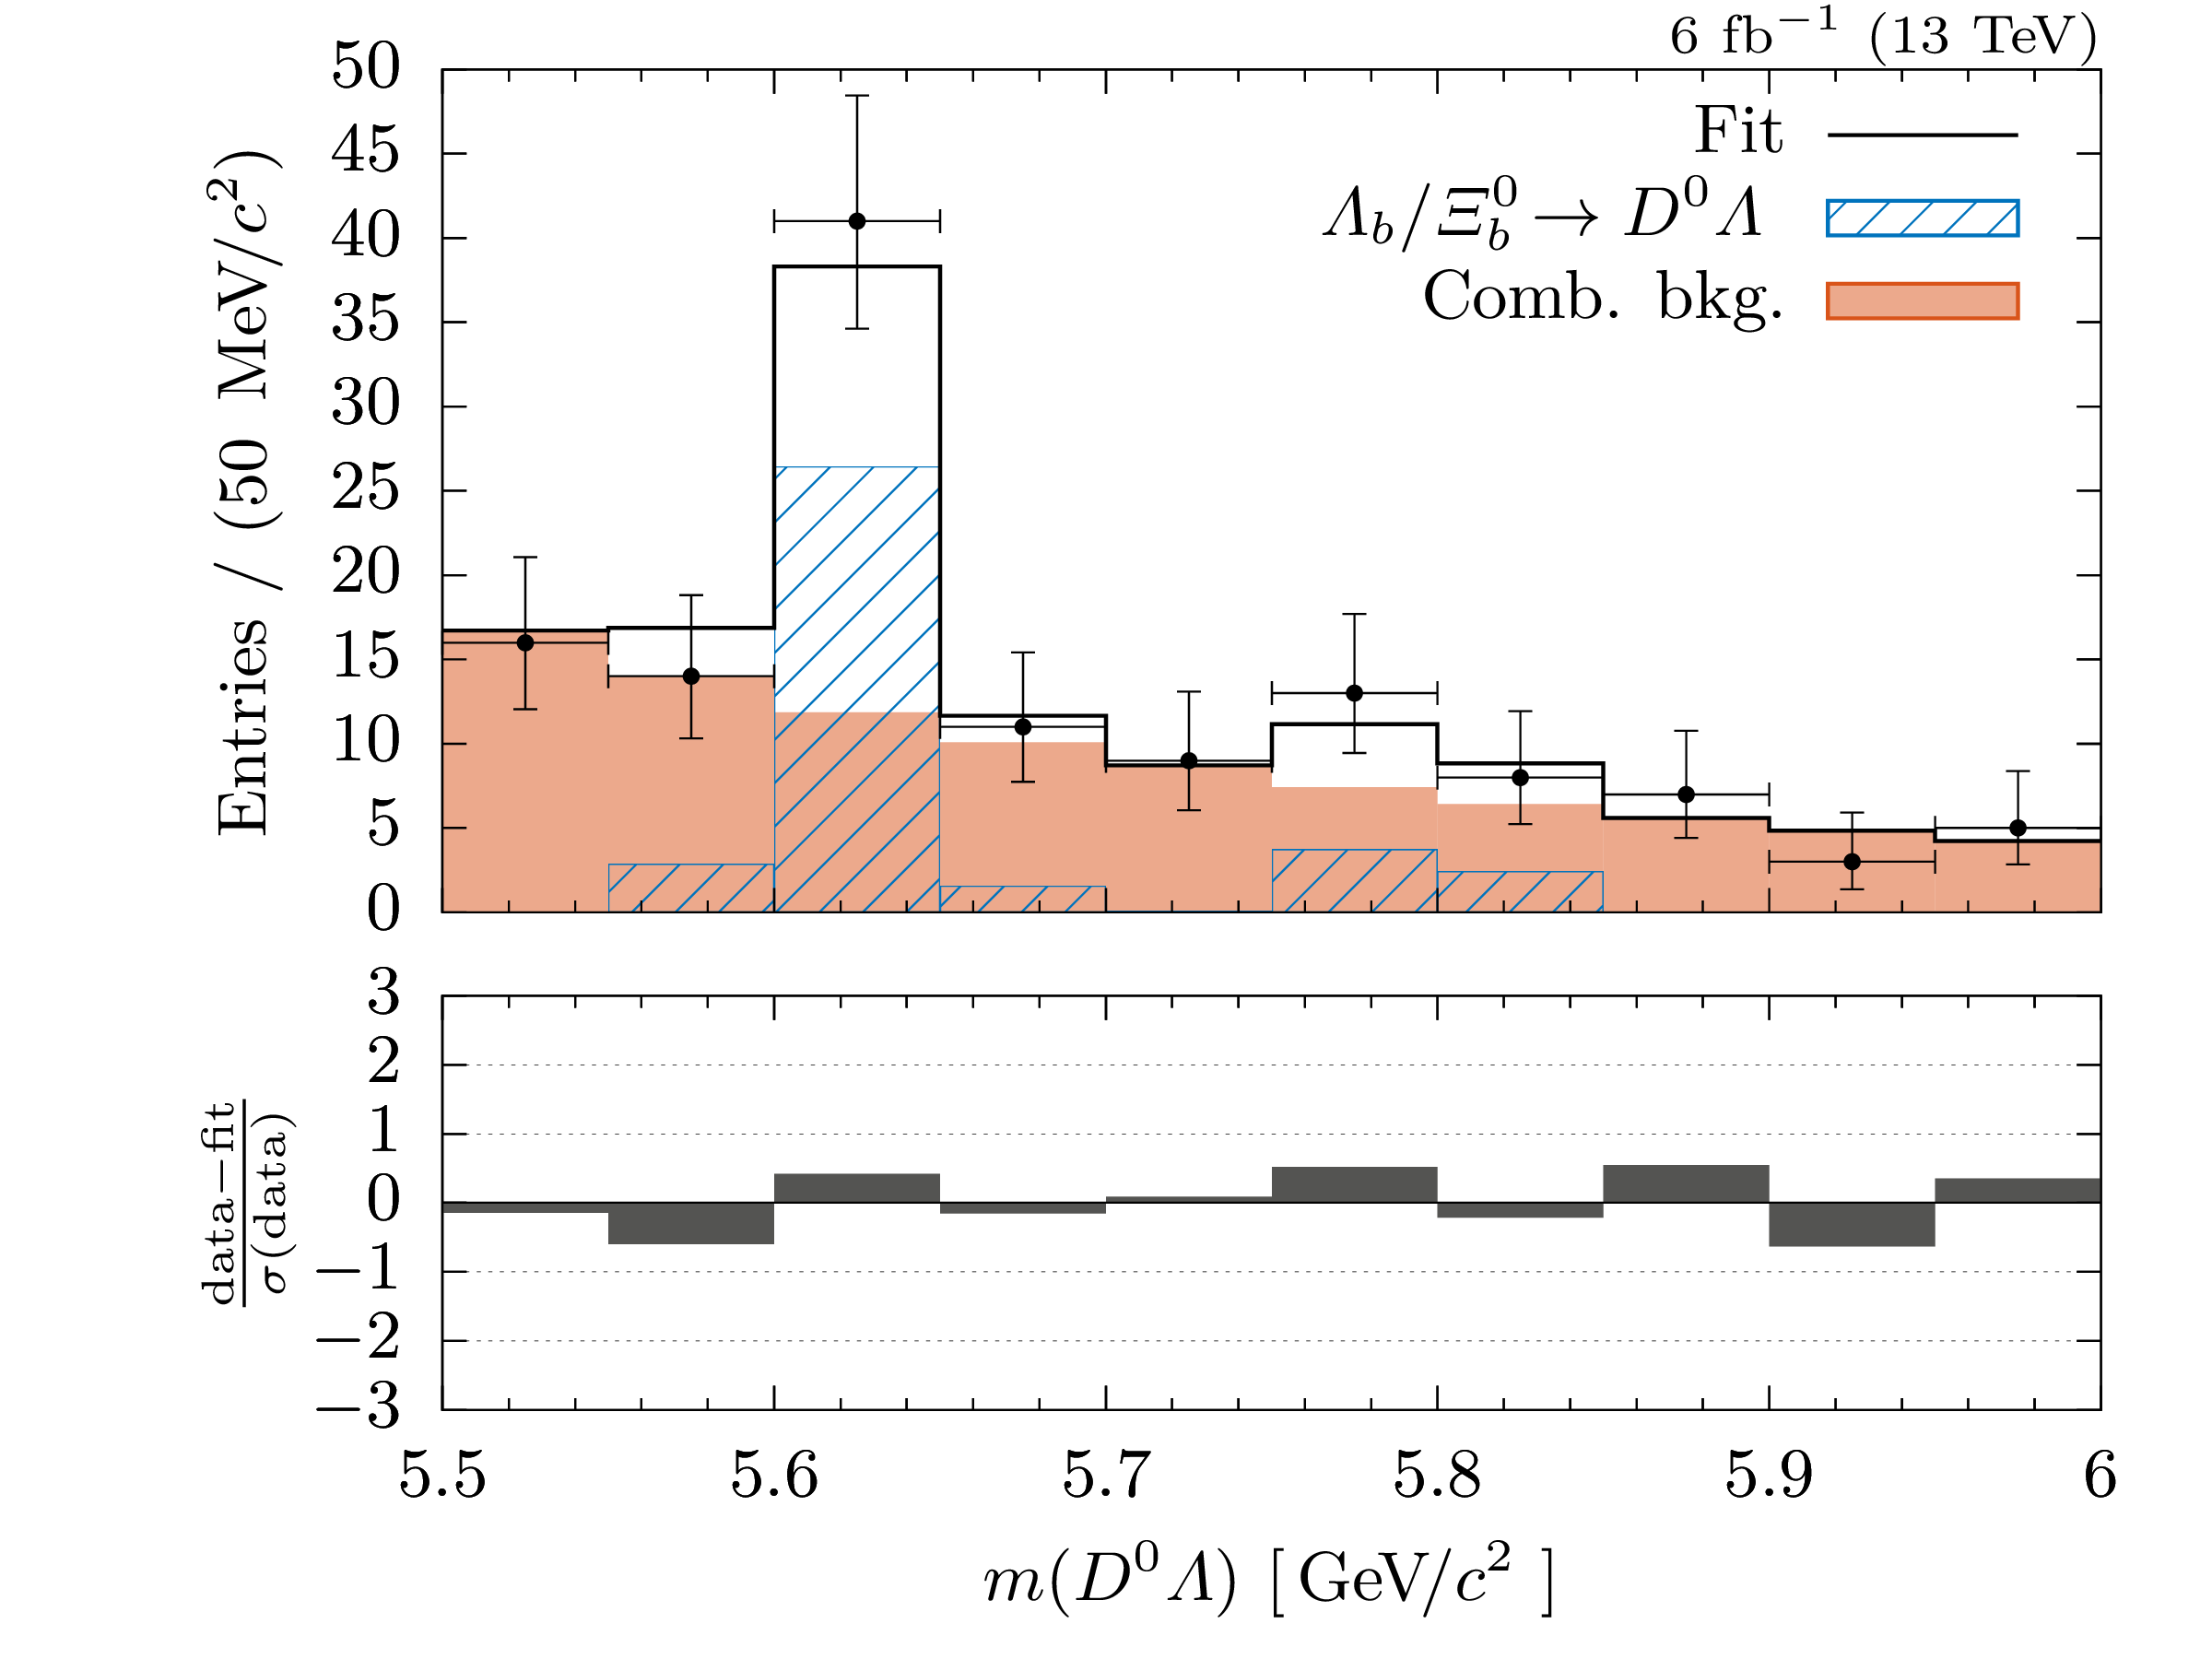
\includegraphics[scale=1.]{fit/hLbM_data_fit1.png}
    \caption{Combined invariant mass of \Dz and \Lz candidates (of both track types), as well as the accumulated projection of the fit in configuration 1. Since $f_2$ is compatible with one (at upper limit), the corresponding \Dstarz background contribution is suppressed (graphically).}
    \label{fig:fit_hLbM_data_fit1}
\end{figure}

\begin{table}
    \centering
    \caption{Corrected yields as obtained from (unbinned, single-entry) likelihood maximization in the configurations 1 and 3 - 7. The extraction and correction of the yields is discussed in Sec.~\ref{sec:fit_yields}.}
    \label{tab:fit_rawyields}
    \begin{tabular}{l%
                    S[separate-uncertainty=true,table-format=2.0(2)]%
                    S[separate-uncertainty=true,table-format=2.0(2)]%
                    S[separate-uncertainty=true,table-format=2.0(2)]%
                    S[separate-uncertainty=true,table-format=1.0(1)]%
                    S[separate-uncertainty=true,table-format=1.1(2)]%
                    S[separate-uncertainty=true,table-format=2.1(2)]}
        \toprule
        & \multicolumn{3}{c}{{\decay{\Lb}{\Dz\Lz}}} & \multicolumn{3}{c}{{\decay{\Xibz}{\Dz\Lz}}} \\
        Configuration & {\gls{LL} \& \gls{DD}} & {\gls{LL}} & {\gls{DD}} & {\gls{LL} \& \gls{DD}} & {\gls{LL}} & {\gls{DD}} \\
        \midrule
        Fit 1 & 31 \pm 7 & 16 \pm 5 & 15 \pm 5 & 6 \pm 4 & 3.2 \pm 2.2 & 3.0 \pm 2.2 \\
        Fit 3 & 32 \pm 7 & 16 \pm 5 & 16 \pm 5 & 6 \pm 4 & 2.8 \pm 2.1 & 2.9 \pm 2.3 \\
        Fit 4 & 32 \pm 7 & 16 \pm 5 & 16 \pm 5 & 6 \pm 4 & 3.1 \pm 2.2 & 2.9 \pm 2.2 \\
        Fit 5 & 32 \pm 7 & 16 \pm 5 & 16 \pm 5 & 6 \pm 4 & 2.9 \pm 2.2 & 2.9 \pm 2.3 \\
        Fit 6 & 32 \pm 7 & 16 \pm 5 & 16 \pm 5 & 6 \pm 4 & 3.0 \pm 2.2 & 3.0 \pm 2.3 \\
        Fit 7a & 32 \pm 7 & 16 \pm 5 & 16 \pm 5 & 6 \pm 4 & 3.1 \pm 2.3 & 2.8 \pm 2.2 \\
        Fit 7b & 32 \pm 7 & 16 \pm 5 & 16 \pm 5 & 6 \pm 4 & 3.0 \pm 2.4 & 3.2 \pm 2.3 \\
        \bottomrule
    \end{tabular}
\end{table}

\section{Yield Extraction}
\label{sec:fit_yields}
According to our definition of the likelihood in Eq.~\eqref{eq:fit_likelihood} the expanded fractions of \decay{\Lb}{\Dz\Lz} and \decay{\Xibz}{\Dz\Lz} are $(1-f_1) \times f_s$ and $(1-f_1) \times (1-f_s)$, respectively.
The yields for each track type are found by multiplication with the amount of recorded events of the given track type $n_\text{LL}$ and $n_\text{DD}$.
Consequently, the accumulated expanded fraction for both track types is given by the weighted sum of the track type dependent fractions where $n_\text{LL}$ and $n_\text{DD}$ are the respective weights.
We note that for estimating the yields by multiplication with $N=n_\text{LL} + n_\text{DD}$, the statistical uncertainty of $n_\text{LL}$ and $n_\text{DD}$ only contributes in $N$, not in the weights since they are part of the chosen (exact) projection of the fit.\footnote{This Poisson part contributes less than $7\,\%$ to the total uncertainty of the estimated yields. The rest is the multinomial error.}
Besides that, we find that ordinary error propagation with the fitted correlations of $f_1$ and $f_s$ and symmetric uncertainties is sufficient due to the low asymmetry of each of the respective asymmetric uncertainties of $3\,\%$ or less.

In order to investigate a possible bias of the yields and to test the validity of the error estimates we run a pseudo-experiment where we draw $N=n_\text{LL} + n_\text{DD}$ random events from the fitted \gls{pdf} (configuration 1) and apply the very same unbinned maximum likelihood fit to these generated data that was used to obtain the parameters of the \gls{pdf} itself. 
In Fig.~\ref{fig:fit_toys_bias} we show the distribution of the fitted yields of the \decay{\Lb}{\Dz\Lz} and \decay{\Xibz}{\Dz\Lz} components after \num{1000} consecutive runs of the outlined technique. (Also see Appx.~\ref{chap:apdx_fitsupp} for more figures of the pseudo-experiments.)
\begin{figure}[htbp]
    \centering
    \begin{subfigure}{.49\textwidth}
        \centering
        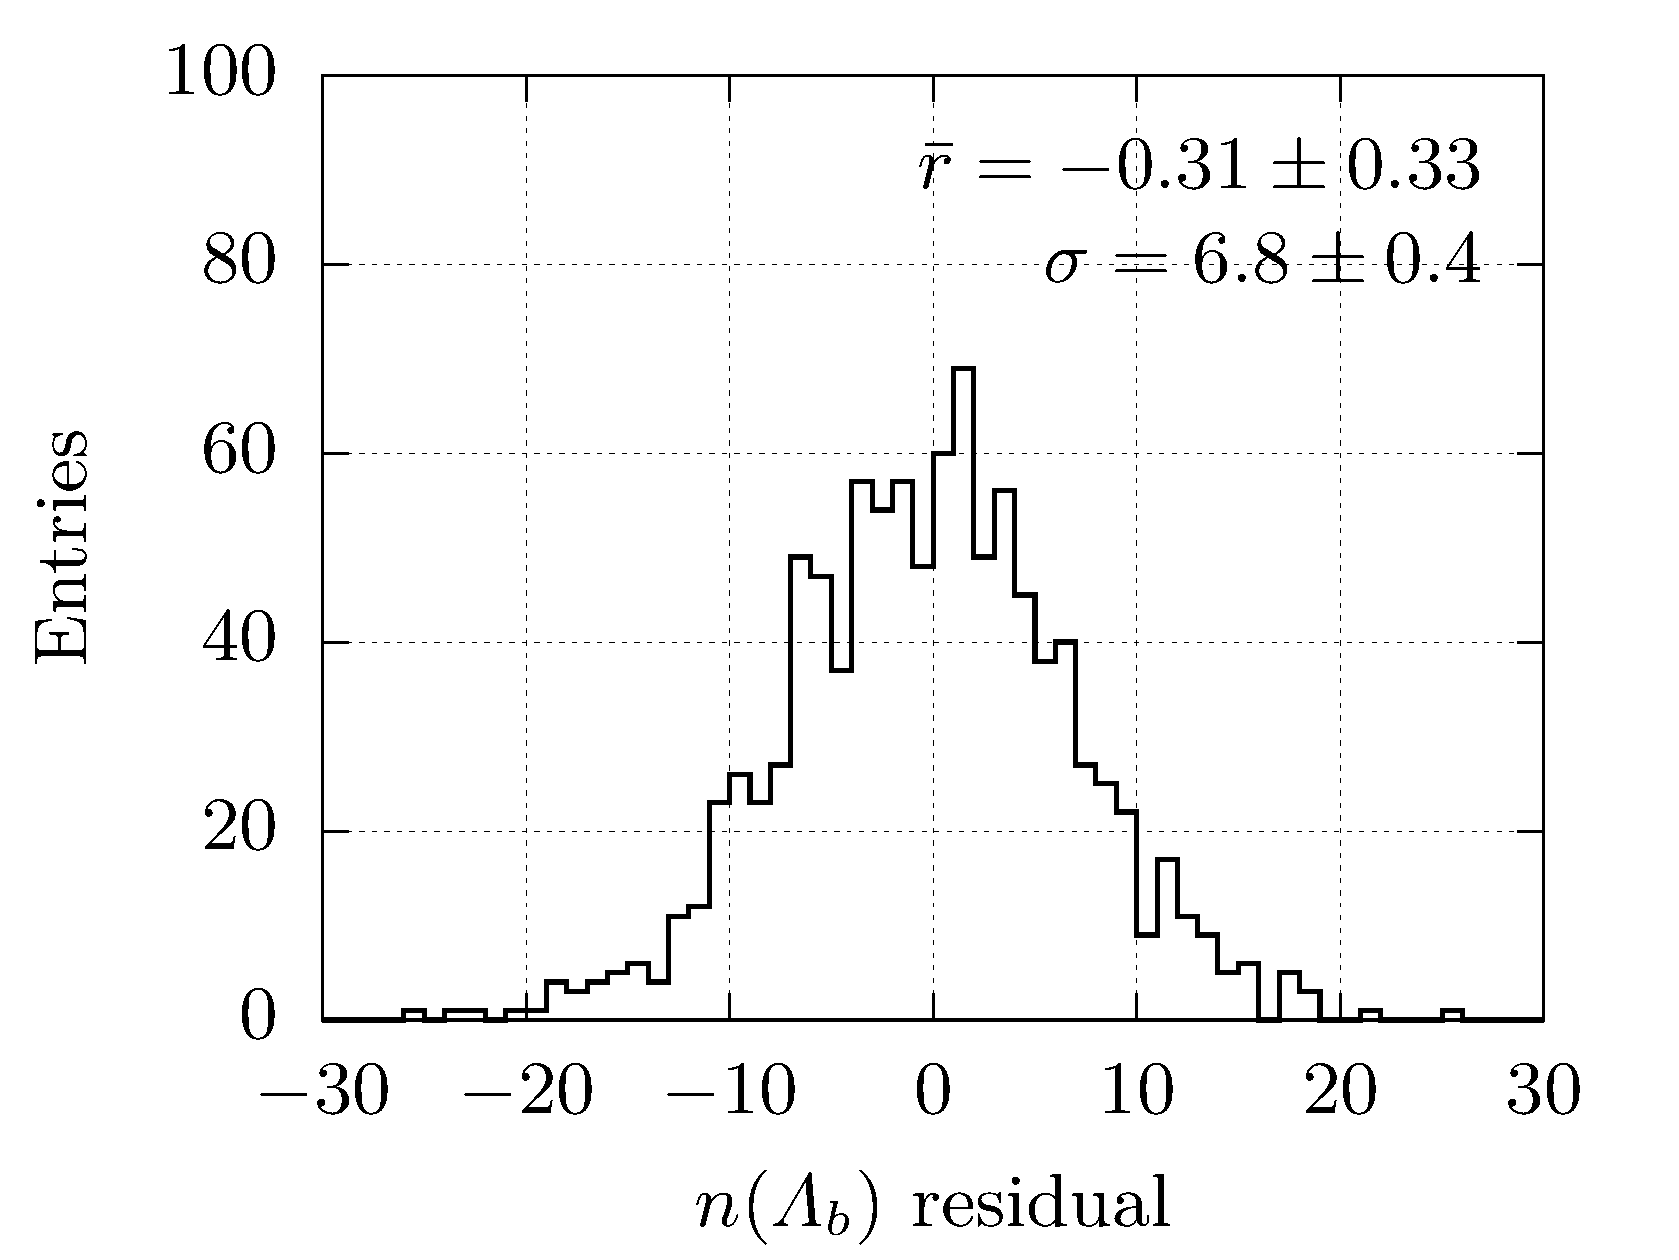
\includegraphics[scale=1.]{fit/hnLb.png}
    \end{subfigure}
    \begin{subfigure}{.49\textwidth}
        \centering
        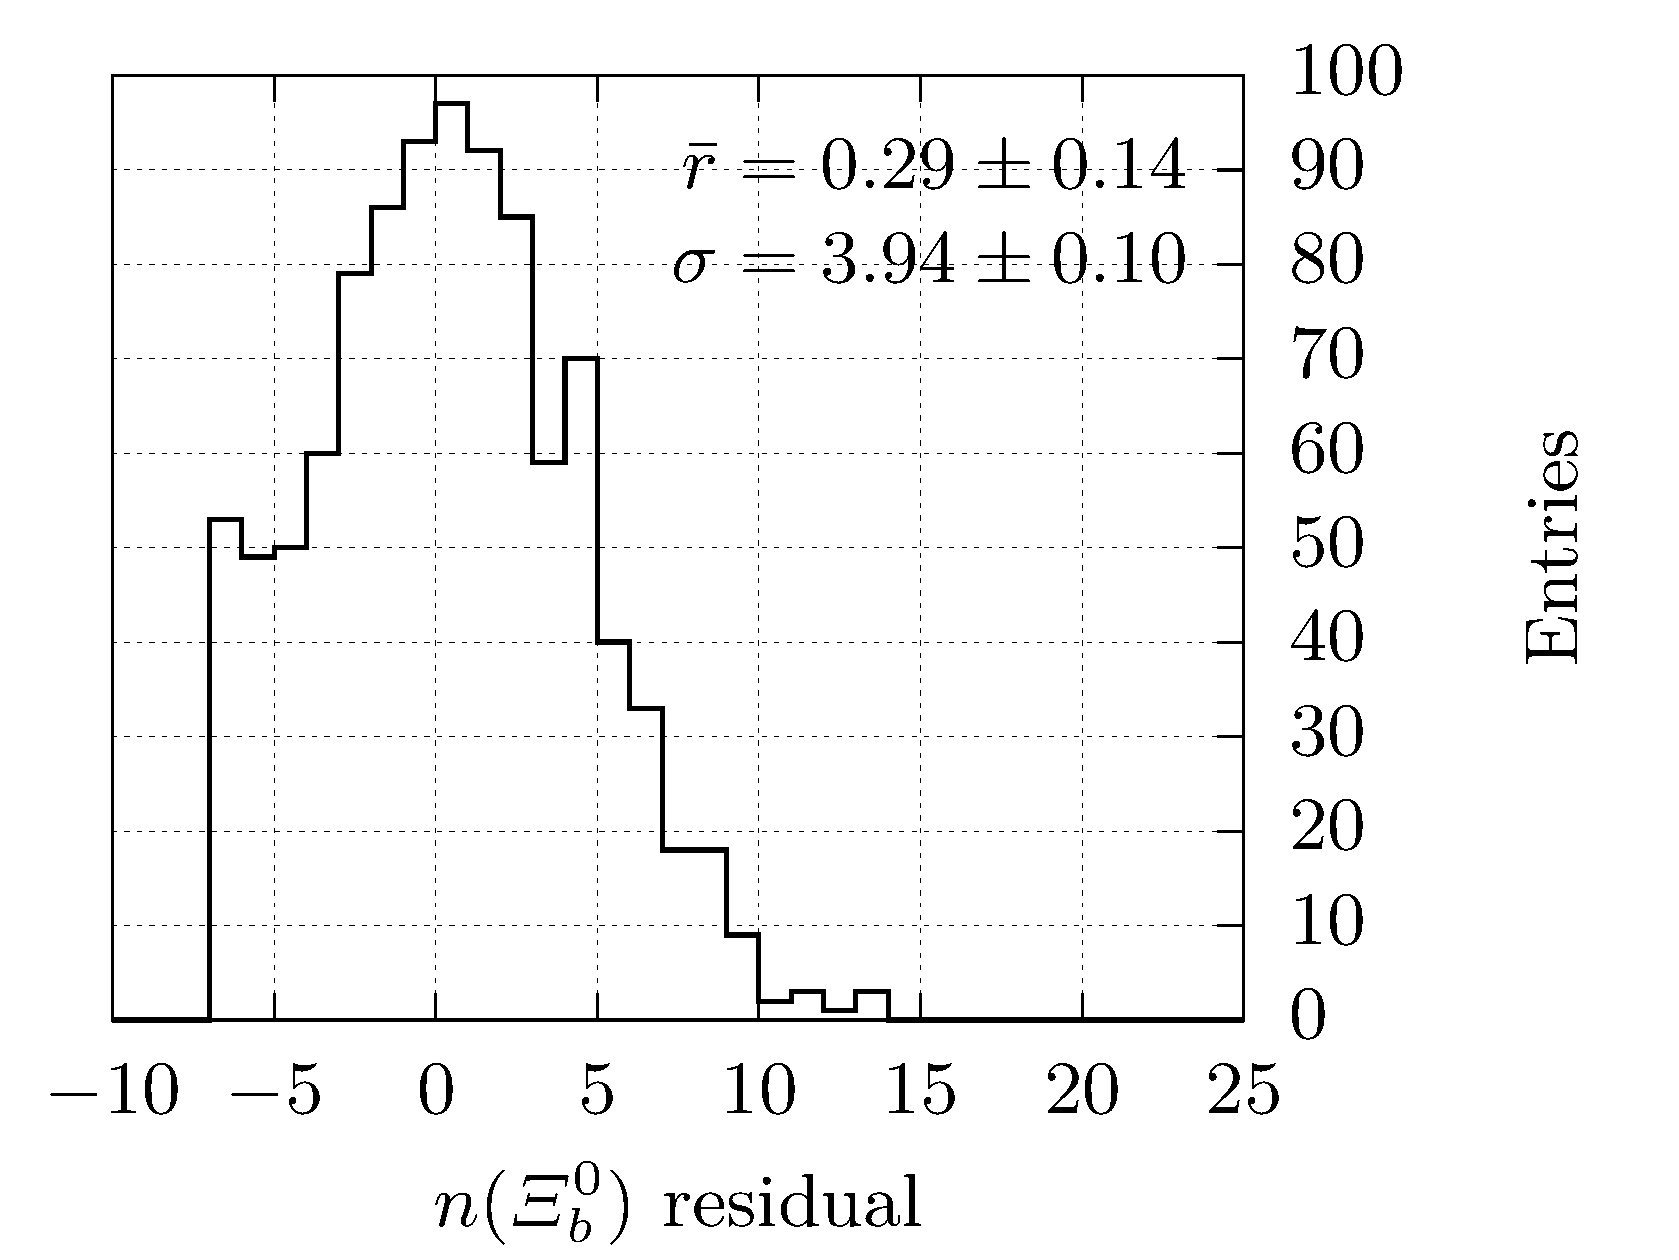
\includegraphics[scale=1.]{fit/hnXib.png}
    \end{subfigure}
    \caption{Difference of the fitted signal yields of pseudo-experiments and recorded data (residual) where the latter was used during generation of the former, as well as the difference of the respective expected and actual sample mean ($\bar r$) and standard deviation ($\sigma$). If $\bar r = 0$ and if the standard deviation is consistent with those found by the fit to recorded data, then the fit is unbiased and has valid error estimations, respectively.}
    \label{fig:fit_toys_bias}
\end{figure}
For an unbiased fit with valid error estimates, both distributions should be distributed according to a clipped Gaussian distribution (\cf{} Appx.~\ref{chap:apdx_clipgaus}).
If so, the sample mean and the standard deviation would follow Eq.~\eqref{eq:apdx_clipgaus_mean} and Eq.~\eqref{eq:apdx_clipgaus_std}, respectively, and the difference of the expected and actual sample mean (referred to as $\bar r$ in Fig.~\ref{fig:fit_toys_bias}) should be compatible with zero.
From Fig.~\ref{fig:fit_toys_bias} we see that the expectations are met for both standard deviations and the mean value of the pseudo-experiments of the \decay{\Lb}{\Dz\Lz} fit, within the respective uncertainties, corresponding to a valid error estimation and an unbiased fit, respectively.
For fitted \decay{\Xibz}{\Dz\Lz} yields though, the results are larger by an offset of $0.29(14)$ on average, which is less than $5\,\%$ of the nominal value.
In a first order approximation we correct for this bias by subtracting fitted yields with the offset.
The corrected signal yields are listed in Tab.~\ref{tab:fit_rawyields}.

\section{Validation of Yield Significances with Pseudo-Experiments}
\label{sec:fit_wilkstest}
When calculating the signal yield significances we made use of Wilks theorem~\cite{wilkstheorem} that states, as the sample size tends to infinity, twice the log-likelihood ratio
\begin{equation*}
    2 \, \log \frac{\mathcal{L}_1}{\mathcal{L}_2} \equiv 2 \, \Delta\!\log \mathcal{L} \,,
\end{equation*}
tends to a $\chi^2$-distribution with $k$ \gls{dof}, where $k$ is the absolute difference of the \gls{dof} of $\mathcal{L}_1$ and $\mathcal{L}_2$.
This approximation works best if all $k$ \gls{dof} are uncorrelated (trivially given for $k=1$), but quickly becomes worse otherwise.
In order to verify the quality of the approximation we again use a pseudo-experiment.
We generate three sample sets where the first consists of instances drawn from the full fitted \gls{pdf}, and the latter two are drawn from a modified \gls{pdf} where $f_s$ is set to zero and one to disable the \Lb and \Xibz signal component, respectively, and $f_1$ is adjusted to retain the same ratio between the remaining signal mode and the combinatorial background~$\mathcal{B}$ (\cf{}~Appx.~\ref{chap:apdx_fitsupp} and in particular Fig.~\ref{fig:fit_toy_pdf_cdf} and Fig.~\ref{fig:fit_hLbM_toy_noLb} for more details).
In total we generate \num{1000} samples for each set and track type, and each sample consists of $50$ ($70$) instances which corresponds to the amount of events of \gls{LL} (\gls{DD}) tracks within the fit range.
Each sample is fitted (in configuration 2, \cf{} Sec.~\ref{sec:fit_model}) and the log-likelihood ratios are calculated.
The resulting distribution of twice these ratios is shown in Fig~\ref{fig:toyfit_deltaL_noLbXib}, as well as the expected (clipped) $\chi^2$-distribution as derived in Appx.~\ref{chap:apdx_clipgaus}.
\begin{figure}[htbp]
    \centering
    \begin{subfigure}{.49\textwidth}
        \centering
        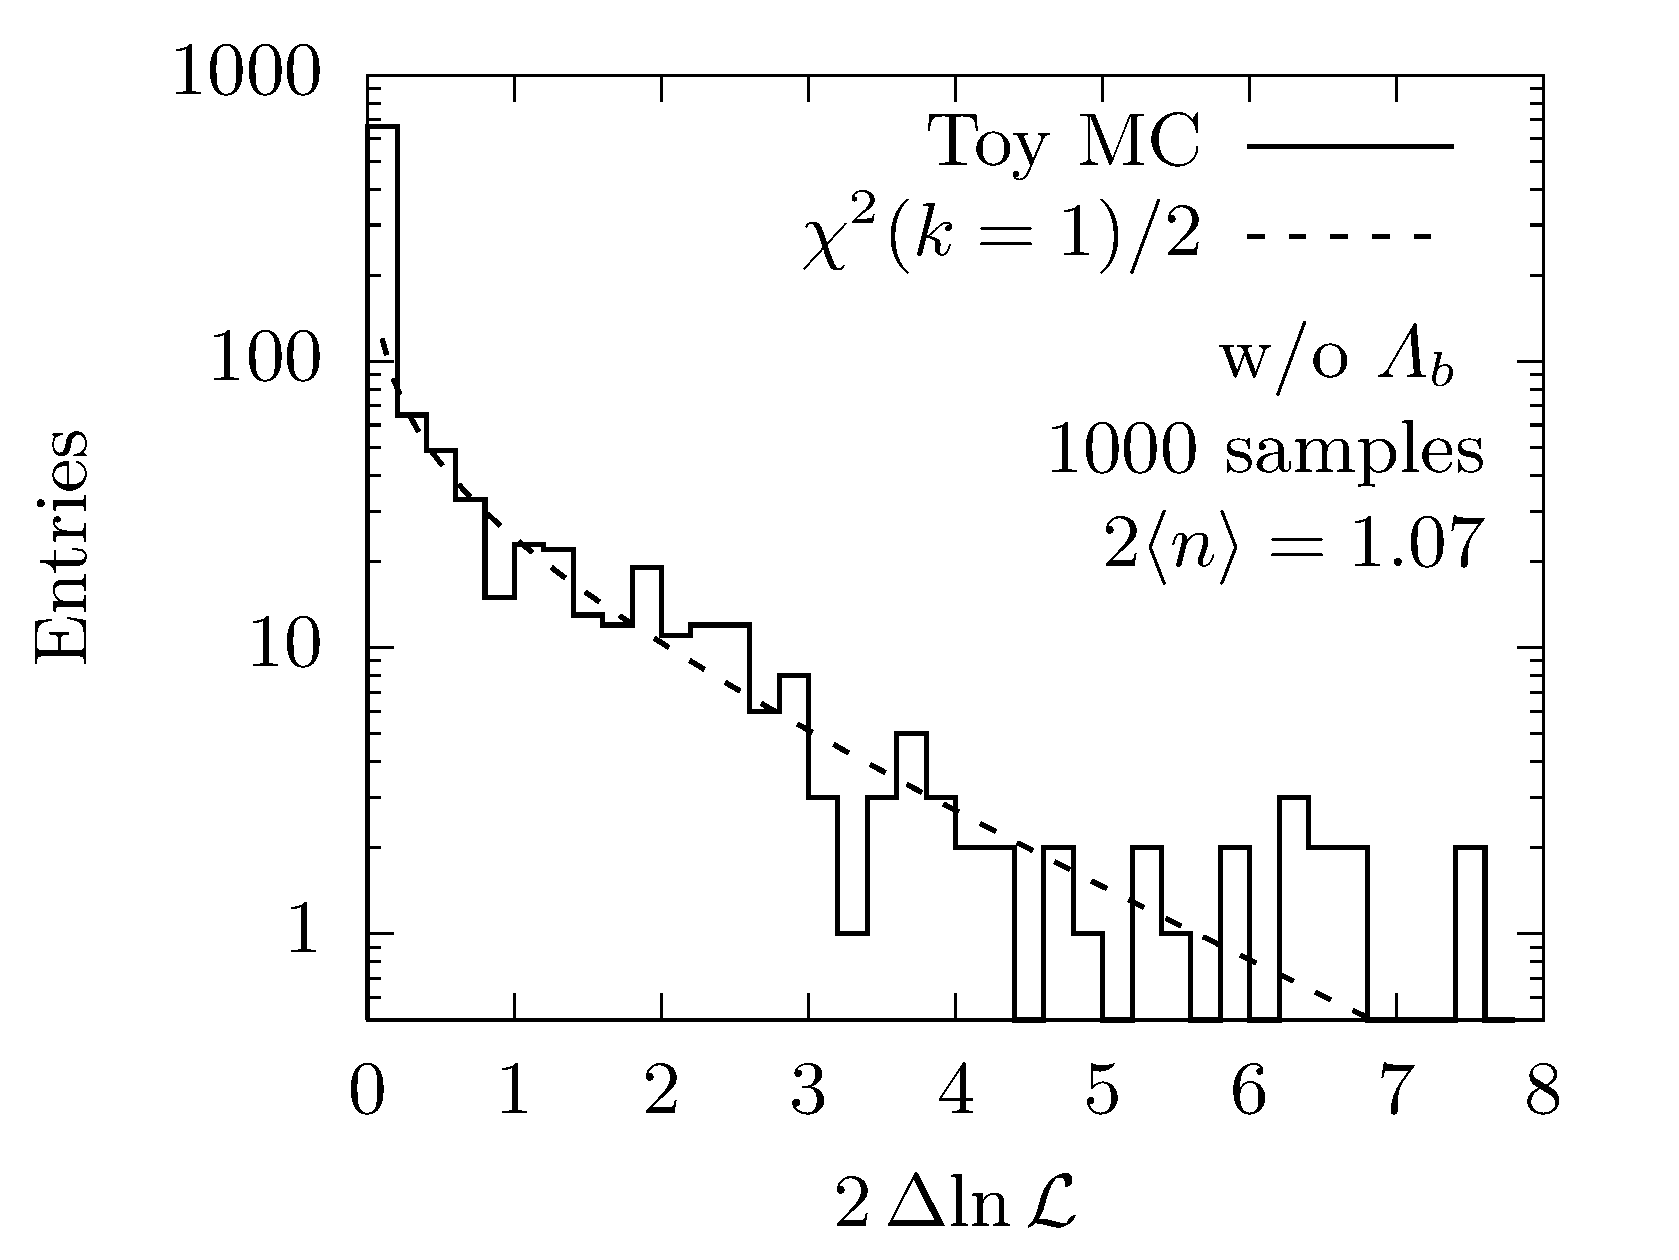
\includegraphics[scale=1.]{fit/deltaL_noLb.png}
    \end{subfigure}
    \begin{subfigure}{.49\textwidth}
        \centering
        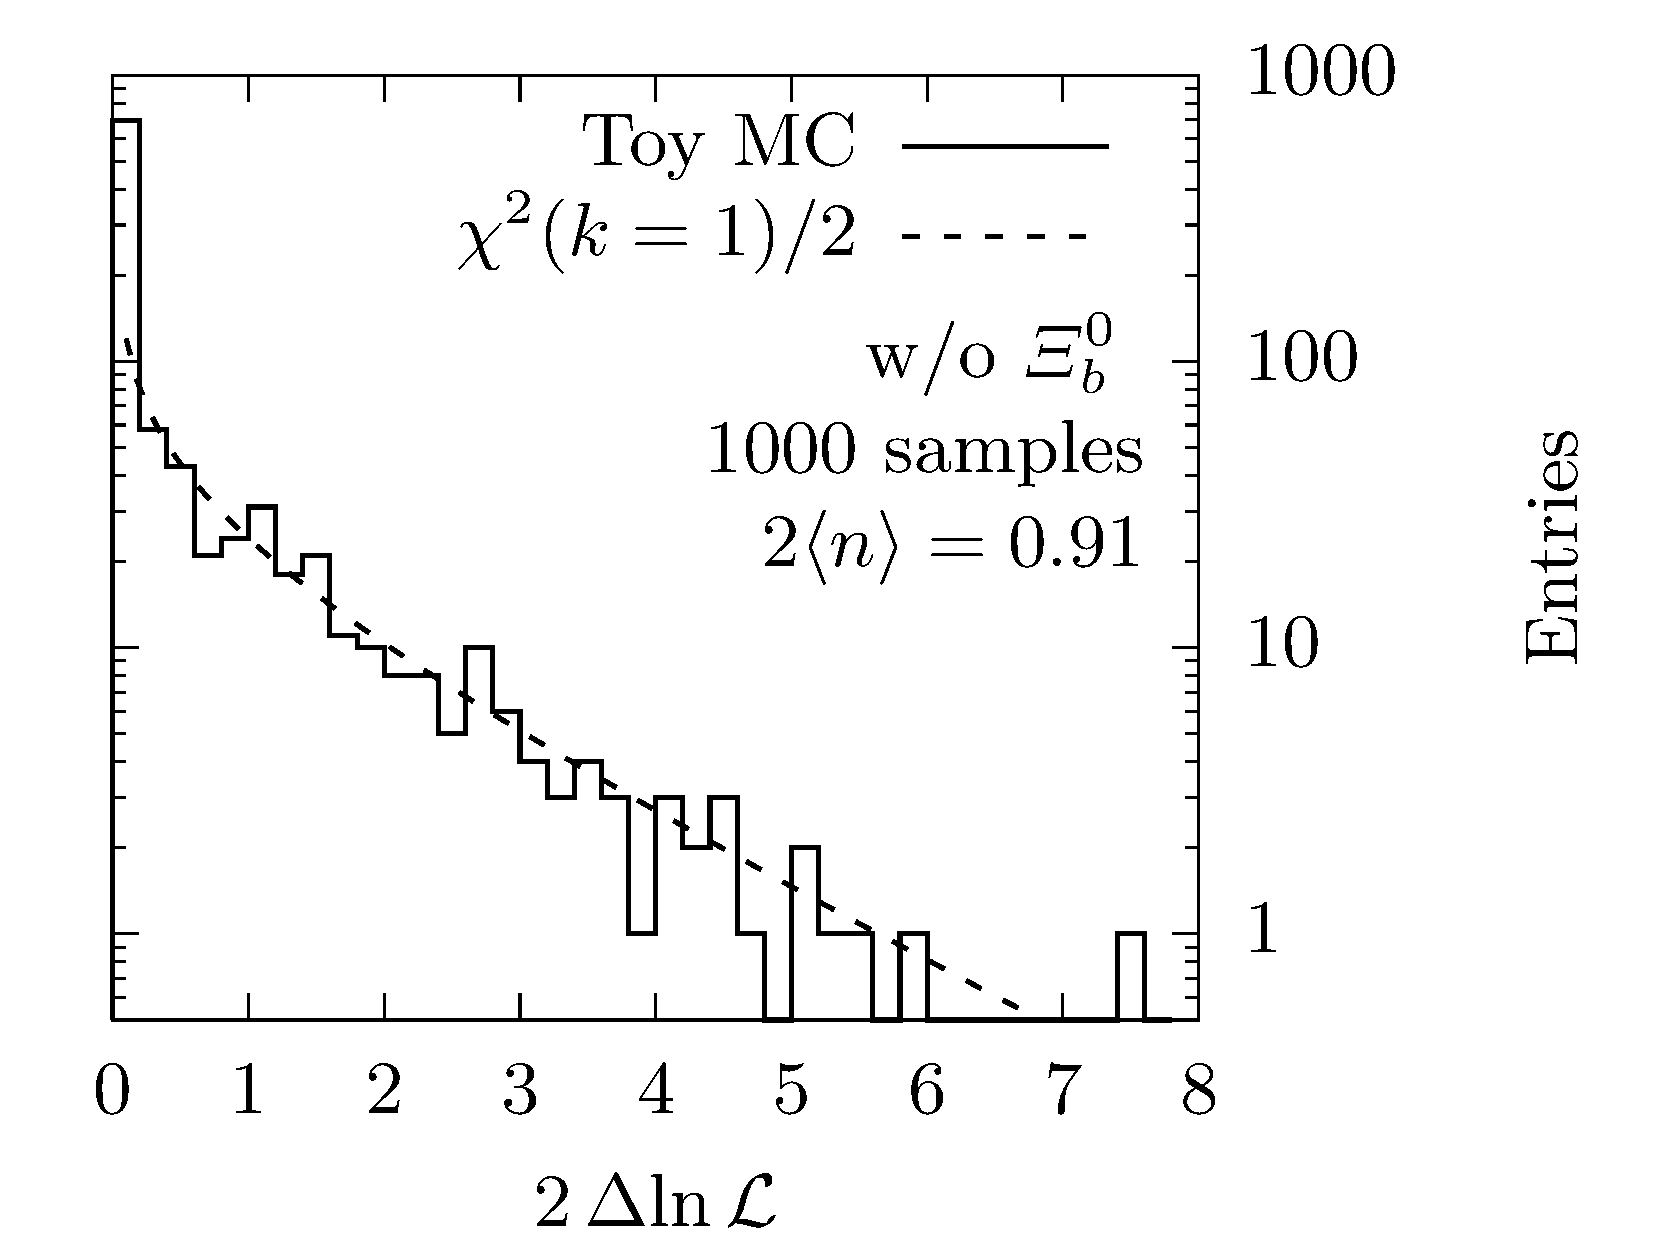
\includegraphics[scale=1.]{fit/deltaL_noXib.png}
    \end{subfigure}
    \caption{Distribution of twice the log-likelihood ratio for \num{1000} samples of a pseudo-experiment (Toy MC) used for validating the estimated \Lb (left) and \Xibz (right) yield significances. The samples are generated under the null hypothesis (no signal) and can thus benchmark our actual observation of twice the log-likelihood ratio of roughly $31$ (left) and $3$ (right). The validity is based on Wilks theorem and is ensured, when the distribution follows a (clipped) $\chi^2$-distribution (dashed line).} 
    \label{fig:toyfit_deltaL_noLbXib}
\end{figure}
The distributions appear to be in good agreement with the expected (clipped) $\chi^2$-distributions and thus validate the estimated yield significance.


\appendix

\begin{frame}[plain,noframenumbering]
    \centering
    \scalebox{2}{BACKUP}
\end{frame}

\backupbegin
\begin{frame}{The CKM matrix}
    \begin{equation*}
        V_\text{\!CKM} = \begin{pmatrix}
        V_{\!ud} & V_{\!us} & V_{\!ub} \\
        V_{\!cd} & V_{\!cs} & V_{\!cb} \\
        V_{\!td} & V_{\!ts} & V_{\!tb}
        \end{pmatrix} = 
        \underbrace{\begin{pmatrix}
        1 - \sfrac{\textcolor{vertexDarkBlue}{\lambda}^2}{2} & \textcolor{vertexDarkBlue}{\lambda} & A \textcolor{vertexDarkBlue}{\lambda}^3 (\rho - \mathrm{i} \textcolor{vertexDarkRed}{\eta}) \\
        -\textcolor{vertexDarkBlue}{\lambda} & 1 - \sfrac{\textcolor{vertexDarkBlue}{\lambda}^2}{2} & A \textcolor{vertexDarkBlue}{\lambda}^2 \\
        A \textcolor{vertexDarkBlue}{\lambda}^3 (1 - \rho - \mathrm{i} \textcolor{vertexDarkRed}{\eta}) & -A \textcolor{vertexDarkBlue}{\lambda}^2 & 1
        \end{pmatrix}}_{\text{\cf{} Wolfenstein: Phys.\,Rev.\,Lett. 51 (1945), 21}}
        + \mathcal{O}(\textcolor{vertexDarkBlue}{\lambda}^3)
    \end{equation*}
    \hfill{\footnotesize $\textcolor{vertexDarkBlue}{\lambda} \approx .23$, $A \approx .81$, $\rho \approx .14$, $\textcolor{vertexDarkRed}{\eta} \approx .35$}
    \begin{itemize}
        \item \underline{One} non-trivial complex phase, encoded in matrix elements
        \begin{itemize}
            \item $V_{\!ub}$ and $V_{\!td}$ (up to $\mathcal{O}(\textcolor{vertexDarkBlue}{\lambda}^2)$)
            \item $V_{\!cd}$, $V_{\!cs}$ and $V_{\!ts}$ (up to $\mathcal{O}(\textcolor{vertexDarkBlue}{\lambda}^6)$)
        \end{itemize}
        \item CP violation if and only if $\textcolor{vertexDarkRed}{\eta} \neq 0$
    \end{itemize}
\end{frame}

\begin{frame}{The CKM Matrix}
    \begin{columns}[T]
        \begin{column}{.75\textwidth}
            \textbf{CP violation (?)}
            \begin{itemize}
                \item If $\eta \neq 0$ some $V_{\!ij}$ carry a complex phase (\textit{weak} phase)
                \begin{itemize}
                    \item amplitude: $\mathcal{A}(\decay{\tquark}{\dquark \Wp}) \sim V_{\!td}^{\textcolor{vertexDarkRed}{*}}$
                    \item amplitude: $\bar{\mathcal{A}}(\decay{\tquarkbar}{\dquarkbar \Wm}) \sim V_{\!td}$
                    \item CPV since $\mathcal{A} \neq \bar{\mathcal{A}}$ (?)
                \end{itemize}
            \end{itemize}
            \ldots~not quite
            \begin{itemize}
                \item Amplitude $\mathcal{A}$ is not observable \ldots
                \item \ldots~but branching fraction $\mathcal{B} \sim |\mathcal{A}|^2$ is
                \begin{itemize}
                    \item CPV needs at least two interfering decay modes with \ldots
                    \item \ldots\;one \textbf{CP odd} and one \textbf{CP even} phase
                \end{itemize}
            \end{itemize}
        \end{column}
        \begin{column}{.25\textwidth}
            \begin{figure}
                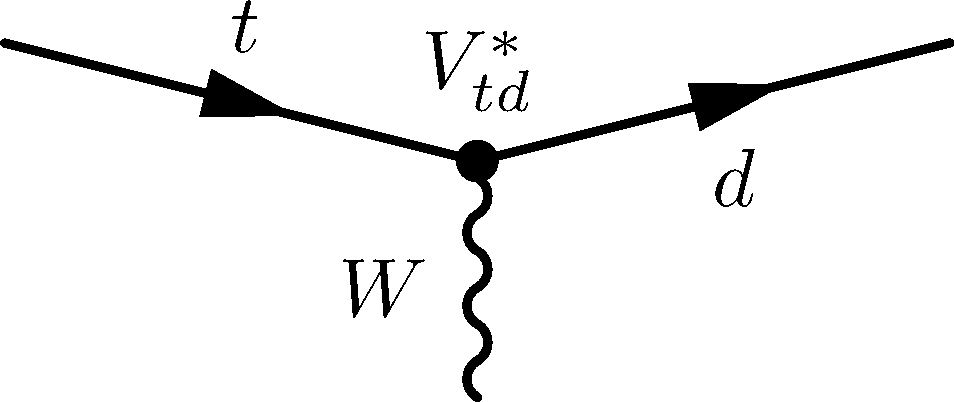
\includegraphics[width=\textwidth]{decay_t2d}
                \caption{\decay{\tquark}{\dquark\Wp}}
            \end{figure}
            \begin{figure}
                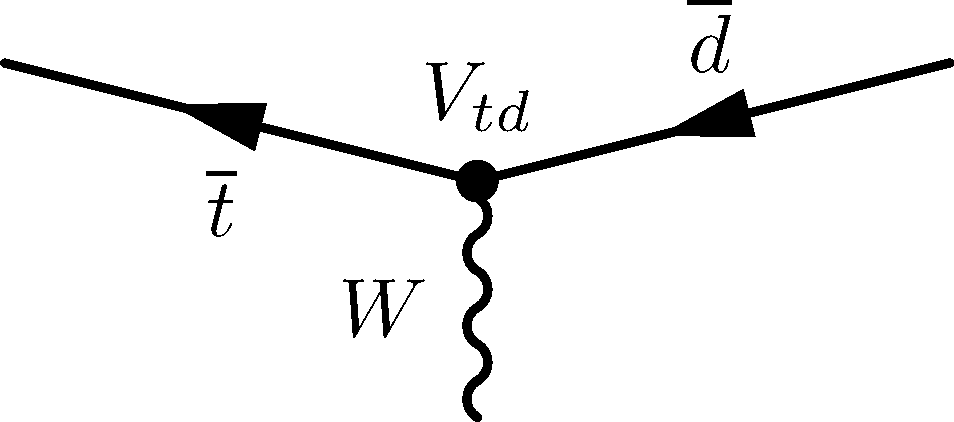
\includegraphics[width=\textwidth]{decay_tb2db}
                \caption{\decay{\tquarkbar}{\dquark\Wm}}
            \end{figure}
        \end{column}
    \end{columns}
\end{frame}

\begin{frame}{Types of CPV}
    \begin{columns}[T]
        \begin{column}{.66\textwidth}
            \begin{column}{.5\textwidth}
                \centering
                \textbf{(1) Direct CPV}
                \begin{equation*}
                    \left| \; 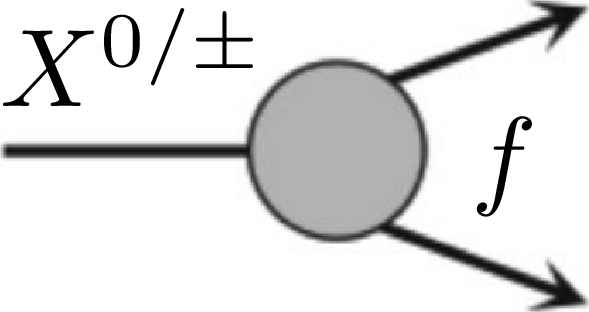
\includegraphics[height=.9cm, valign=c]{cpv1.png} \; \right|^2
                \end{equation*}
                \scalebox{1.5}{$\neq$}
                \begin{equation*}
                    \left| \; 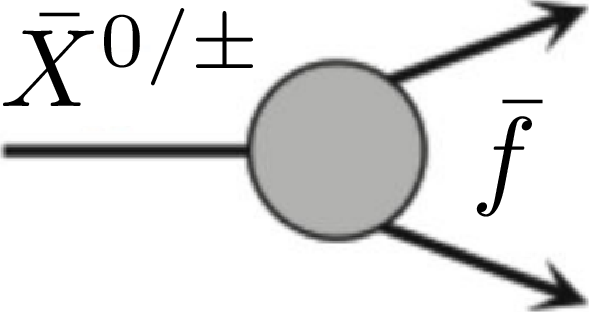
\includegraphics[height=.9cm, valign=c]{cpv1bar.png} \; \right|^2
                \end{equation*}
            \end{column}
            \begin{column}{.5\textwidth}
                \centering
                \textbf{(2) CPV in mixing}
                \begin{equation*}
                    \left| \; 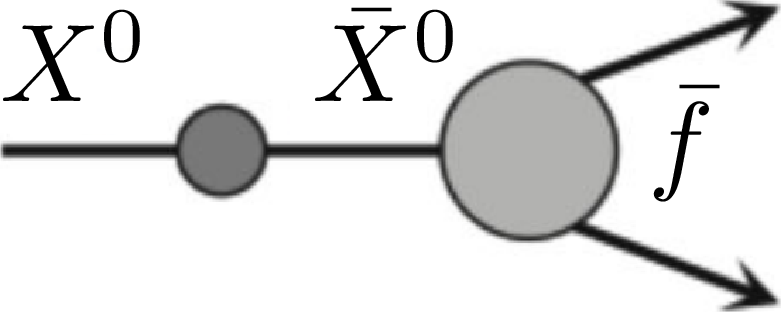
\includegraphics[height=.9cm, valign=c]{cpv2.png} \; \right|^2
                \end{equation*}
                \scalebox{1.5}{$\neq$}
                \begin{equation*}
                    \left| \; 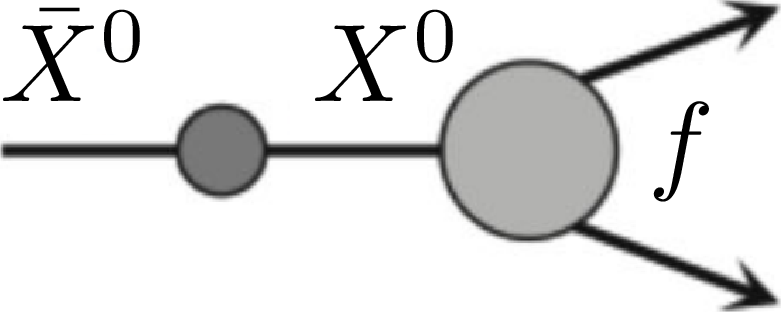
\includegraphics[height=.9cm, valign=c]{cpv2bar.png} \; \right|^2
                \end{equation*}
            \end{column}

            \vspace{5mm}
            \begin{itemize}
                \item CP odd: from CKM matrix
                \item CP even:
                \begin{itemize}
                    \item (1): strong phase difference between both amplitudes (\eg{}, \textit{tree} and \textit{penguin})
                    \item (2), (3): $\pi / 2$ (\textbf{constant!})
                \end{itemize}
            \end{itemize}
        \end{column}
        \begin{column}{.33\textwidth}
            \centering
            \textbf{(3) CPV in interference of mixing and decay}
            \begin{equation*}
                \left| \; 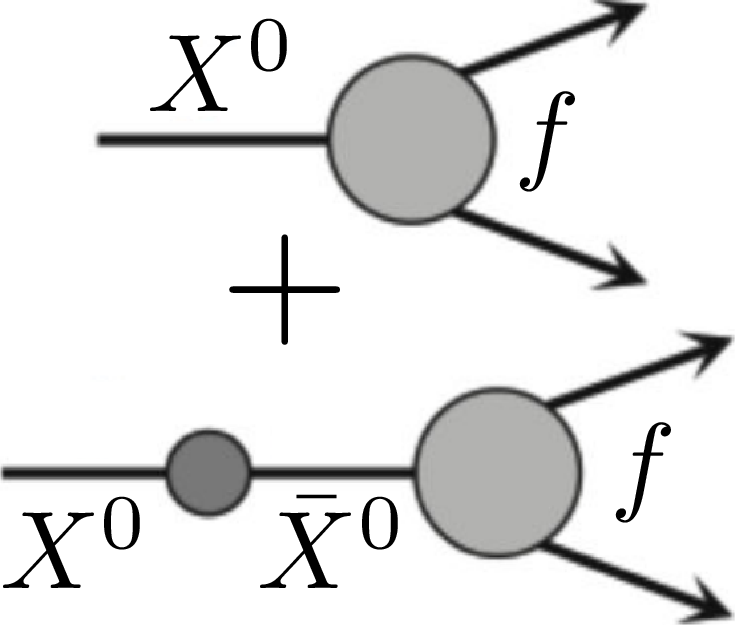
\includegraphics[height=1.8cm, valign=c]{cpv3.png} \; \right|^2
            \end{equation*}
            \scalebox{1.5}{$\neq$}
            \begin{equation*}
                \left| \; 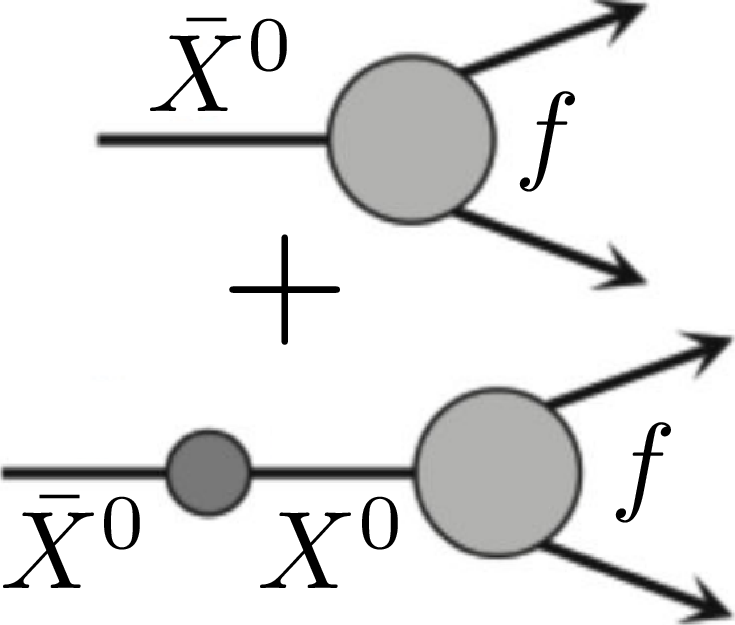
\includegraphics[height=1.8cm, valign=c]{cpv3bar.png} \; \right|^2
            \end{equation*}
            {\tiny \hfill(Images: \textit{CP Violation}, I.\,I. Bigi and A.\,I. Sanda)}
        \end{column}
    \end{columns}
\end{frame}

\begin{frame}{The CKM Matrix}
    \textbf{Another parametrization}
    -- {\footnotesize Prog. Part. Nucl. Phys. 47 (2001)}
    \begin{columns}
        \begin{column}{.7\textwidth}
            \begin{equation*}
                V_\text{\!CKM} = \begin{pmatrix}
                \phantom{-}|V_{\!ud}|\phantom{\mathrm{e}^{-\mathrm{i}\phi_6}} &
                \phantom{-}|V_{\!us}|\phantom{\mathrm{e}^{-\mathrm{i}\phi_6}} &
                \phantom{-}|V_{\!ub}| \mathrm{e}^{-\mathrm{i}\tilde\gamma}\\
                -|V_{\!cd}| \mathrm{e}^{+\mathrm{i}\phi_4} &
                \phantom{-}|V_{\!cs}| \mathrm{e}^{-\mathrm{i}\phi_6} &
                \phantom{-}|V_{\!cb}|\phantom{\mathrm{e}^{-\mathrm{i}\tilde\gamma}} \\
                \phantom{-}|V_{\!td}| \mathrm{e}^{-\mathrm{i}\tilde\beta\phantom{{}_4}} &
                -|V_{\!ts}| \mathrm{e}^{+\mathrm{i}\phi_2} &
                \phantom{-}|V_{\!tb}|\phantom{\mathrm{e}^{-\mathrm{i}\tilde\gamma}}
                \end{pmatrix}
            \end{equation*}
        \end{column}
        \begin{column}{.3\textwidth}
            \scalebox{.75}{\parbox{\linewidth}{%
            \begin{align*}
                &\gamma \equiv \tilde\gamma - \phi_4, & \phi_\mathbf{2} &\approx \eta \textcolor{vertexDarkBlue}{\lambda}^\mathbf{2}\\
                &\beta \equiv \tilde\beta + \phi_4, & \phi_\mathbf{4} &\approx \eta A^2 \textcolor{vertexDarkBlue}{\lambda}^\mathbf{4}\\
                &\alpha \equiv \pi - \beta - \gamma, & \phi_\mathbf{6} &\approx \eta A^4 \textcolor{vertexDarkBlue}{\lambda}^\mathbf{6}\\
                &\beta_s \equiv \phi_s \equiv \phi_2 + \phi_6
            \end{align*}}}
        \end{column}
    \end{columns}
    \vfill
    \begin{columns}[T]
        \begin{column}{.6\textwidth}
            \begin{itemize}
                \item From unitarity: 6 triangles
                \begin{itemize}
                    \item $V_{\!ud} V^*_{\!us} \,+\, V_{\!cd} V^*_{\!cs} \,+\, V_{\!td} V^*_{\!ts} = 0$
                    \item $V_{\!ud} V^*_{\!ub} \,+\, V_{\!cd} V^*_{\!cb} \,+\, V_{\!td} V^*_{\!tb} = 0$
                    \item \ldots~4 more 
                \end{itemize}
                \item Angles $\tilde\alpha$, $\tilde\beta$, $\tilde\gamma$ and $\phi_{2,4,6}$ \textbf{depend on phase convention} (\ie{}, not observable)
                \item Phases of products $V_{\!ij} V_{\!kl} V^*_{\!il} V^*_{kj}$ are \textbf{invariant} and \textbf{observable} (\eg{}, $\alpha$, $\beta$, $\gamma$, \ldots)
            \end{itemize}
        \end{column}
        \begin{column}{.4\textwidth}
            \hfill
            $V_{\!ud} V^*_{\!ub} + V_{\!cd} V^*_{\!cb} + V_{\!td} V^*_{\!tb} = 0$\\
            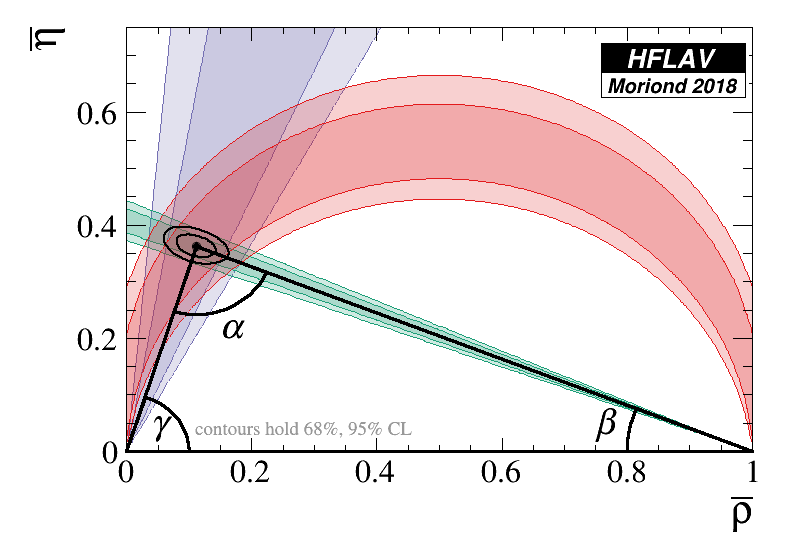
\includegraphics[width=\textwidth]{hflav_rhoeta18}
        \end{column}
    \end{columns}
\end{frame}

\begin{frame}{Probing the SM by Overconstraining}
    \begin{columns}
        \begin{column}{.55\textwidth}
            \begin{itemize}
                \item \textbf{Motivation:}
                \begin{itemize}
                    \item We utterly fail explaining CPV on cosmological scale!
                    \item Is the CKM matrix the only source of CPV?
                    \item Is the SM incomplete / are there more particles?
                \end{itemize}

                \item \textbf{Strategy:}
                \begin{itemize}
                    \item Overconstrain CKM triangles by measuring
                    \begin{itemize}
                        \item sides -- \eg{}, $|V_{\!td} V^*_{\!tb}|$
                        \item angles -- \eg{}, $\gamma = \arg \left( -\frac{V_{\!ud} V^*_{\!ub}}{V_{\!cd} V^*_{\!cb}} \right)$
                    \end{itemize}
                    \item Is $\beta_s = \arg \left( -\frac{V_{\!ts} V^*_{\!tb}}{V_{\!cs} V^*_{\!cb}} \right)$  tiny? ($\mathcal{O}(\textcolor{vertexDarkBlue}{\lambda}^2)$)
                \end{itemize}
            \end{itemize}
        \end{column}
        \begin{column}{.45\textwidth}
            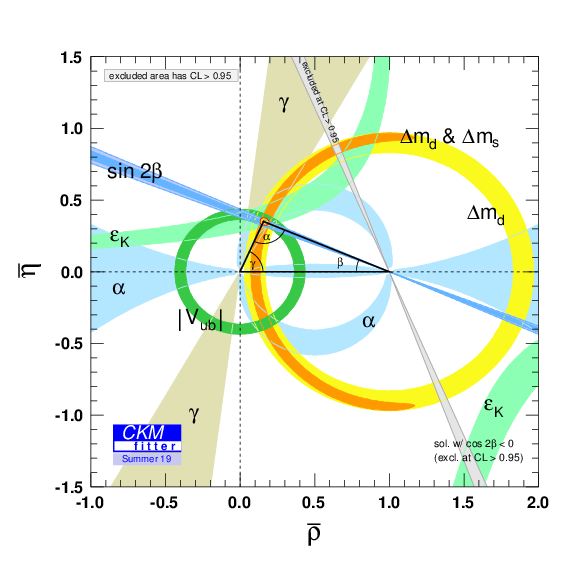
\includegraphics[width=\textwidth]{ckmfitter}
        \end{column}
    \end{columns}

    \centering
    \scalebox{1.2}{Any deviation would point towards \textbf{new physics}, \eg{}, 4th quark family?}
\end{frame}

\begin{frame}{Branching ratios}
    \centering
    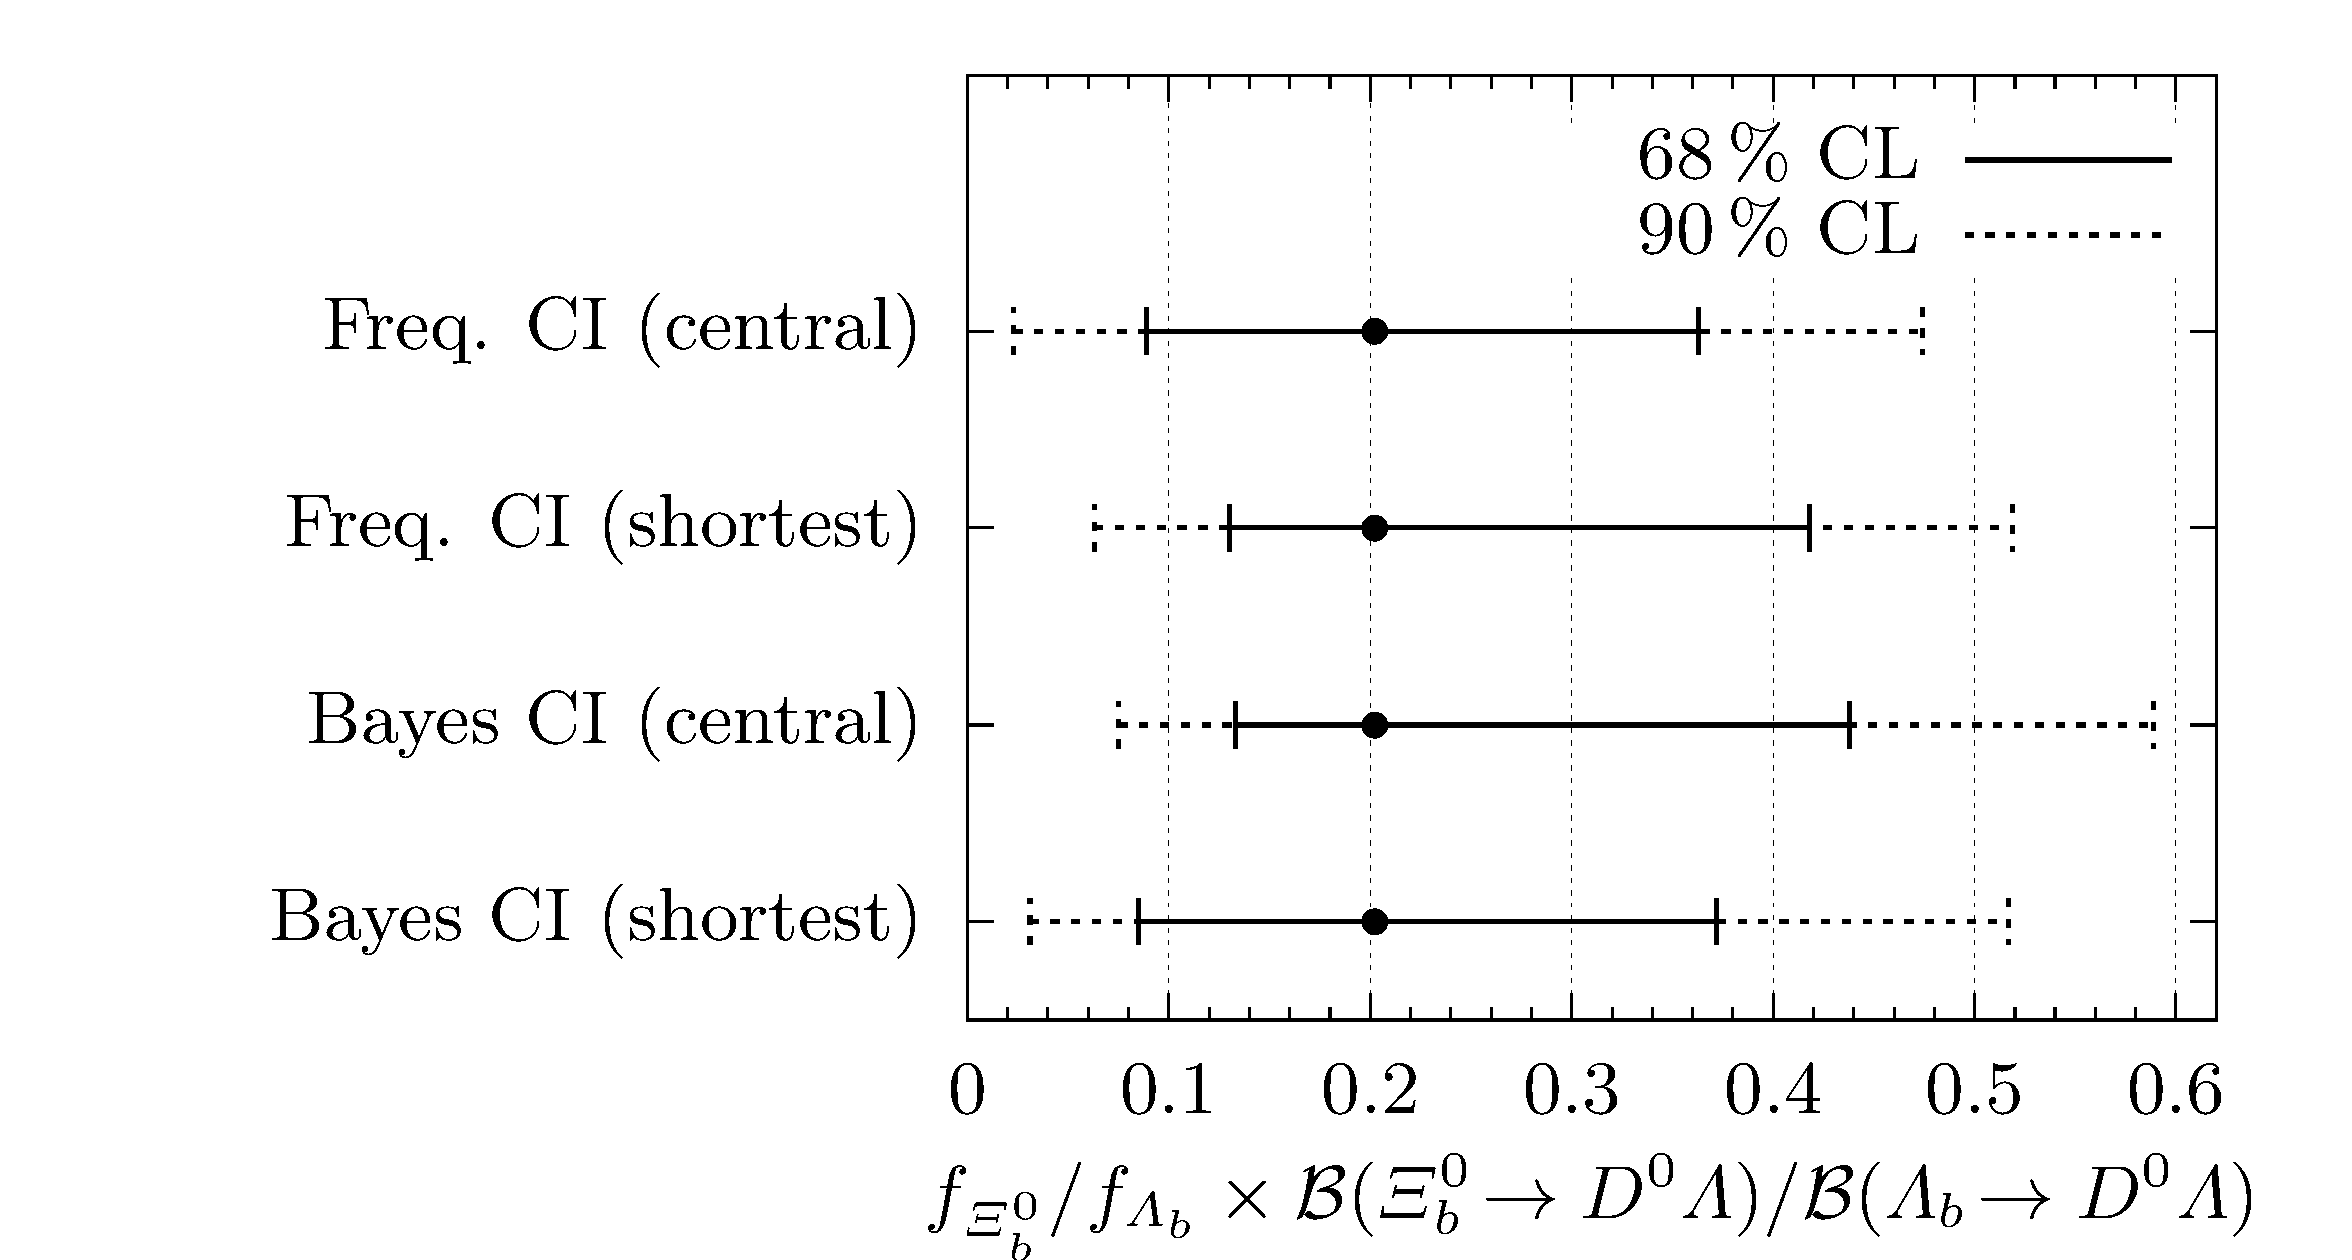
\includegraphics[scale=1.]{br/xiblb_brs.png}
\end{frame}

\backupend

\end{document}
